\documentclass[12pt]{article}
%\usepackage{natbib}
\usepackage[numbers]{natbib}
\usepackage{amsthm}
\usepackage[toc,page]{appendix}
\usepackage{color}
\usepackage{graphicx}
\usepackage{tabularx}
\usepackage{caption}

\usepackage{longtable}
\usepackage[]{inputenc}
\usepackage[T1]{fontenc}
\usepackage{fullpage}
\usepackage{coqdoc}
\usepackage{amsmath,amssymb}
\usepackage{listings}


\DeclareGraphicsExtensions{.pdf,.png,.jpg}
\definecolor{codegreen}{rgb}{0,0.6,0}
\definecolor{codegray}{rgb}{0.5,0.5,0.5}
\definecolor{codepurple}{rgb}{0.58,0,0.82}
\definecolor{backcolour}{rgb}{0.95,0.95,0.92}

\DeclareCaptionFormat{listing}{#1#2#3}
\captionsetup[lstlisting]{format=listing,singlelinecheck=false} 

\lstdefinestyle{mystyle}{
    backgroundcolor=\color{backcolour},   
    commentstyle=\color{codegreen},
    keywordstyle=\color{magenta},
    numberstyle=\tiny\color{codegray},
    stringstyle=\color{codepurple},
    basicstyle=\footnotesize,
    breakatwhitespace=false,         
    breaklines=true,                 
    captionpos=b,                    
    keepspaces=true,                 
    numbers=left,                    
    numbersep=5pt,                  
    showspaces=false,                
    showstringspaces=false,
    showtabs=false,                  
    tabsize=2
}
\newtheorem{mydef}{Definition}



\begin{document}

\title{Self-Affinity in Source Code : A Programmer Metric}
\author{Ben  Goodspeed}

\maketitle
\pagebreak


%TODO consider whether to make all interpretation speculative
%TODO use the benchmark stuff from alioth (lang shootout thing) for further study
%TODO look into 'voice', passive vs active in all cases.  see which is 'right' for a given journal.
\begin{abstract}
%TODO abstract here
Fractal self-affinity of source code text is calculated by multifractal detrending analysis.  This affinity is discussed in the context of software quality and complexity metrics.  It is focused on the programmer's view of the source code.  It is shown to have language independence properties, but suffers in universal applicability.  Deliberate inattention to semantics of the source language shows both benefits and detriments to the utility of the affinity as a metric.
\end{abstract}

\tableofcontents
\listoffigures

\pagebreak
\section{Introduction}
Some source code is easy to follow (and thus easy to maintain, to fix and to extend).  Other code is not easy to follow.  Programmers have an intuition for detecting "bad" \cite{Feathers:WEWLC:04, 
Martin:CleanCode:08}
 code.  Sometimes this is due to certain patterns (often called "smells" \cite{Fowler:Refactoring:99}) within the source code.

\lstset{language=C}

\begin{figure}[h]
\centering
\begin{minipage}[b]{0.40\linewidth}
\begin{lstlisting}[frame=single][caption=My caption]
long simple(int a) {
     long b = a * 300;
     return a + b + 2;
}
\end{lstlisting} 

\caption{Simple Code}
\label{fig:minipage1}
\end{minipage}
\quad
\begin{minipage}[b]{0.55\linewidth}
\begin{lstlisting}[frame=single]
long complex(int a, int b, long c) {
     if (a == b) {
         while(b) {
#ifdef CONST         
             continue;
#else
             if (c == a) return -1;
#endif
        }  }
    return 0;
}
\end{lstlisting} 
\caption{Complex Code}
\label{fig:minipage2}
\end{minipage}
\end{figure}

Notice that the code on the left looks easy to follow, whereas the code on the right looks more difficult to comprehend.
This intuition is valuable as it gives a sense of when code will be difficult to change, or where changes may have unintended consequences.  However, the qualitative nature of these descriptions makes it difficult to compare between two programmers judgments of code.  Many software complexity metrics have been described intending to make this value judgment more quantitative (for example \cite{Radjenovic:SoftwareMetrics:13, McCabe:SoftwareComplexity:76, Concas:FractalSoftware:06, Valverde:SmallWorlds:03}), and some of these are discussed in section \ref{RelatedWork}.


The main problem is making a judgment call about qualitative things explicit and consistent across languages, platforms and between different people.

If an intuition or judgment about source code is not numerical and reproducible by other people, we can't compare the results.  Two pieces of bad code are both just "bad", we can't use it to make precise what is bad about them, or describe exactly how "bad".

We would like to be able to assign a normalized (in this case between 0.5 and 1) numeric value to the complexity of a piece of code.  We want this value to be applicable to whatever portion of the code we analyze, whether considering the source file in its entirety or just a single method.  In a related sense, we'd like to know if the characterization we get from examining a single method is representative of the whole.

This sense of multi-scale similarity is at the core of fractal analysis \cite{Peitgen:FractalsForClassroom:91}
\cite{Kantelhardt:DFA:01}.

Since there are so many programming languages, evaluating which one might be suitable for a given task is a challenge.  The reality of modern programming is that very few current projects are mono-linguistic, but rather they are often polyglot.

For example there is currently a trend towards web-based delivery of software.  Given the popularity of the platform, a number of languages and frameworks exist to develop these web applications.  Python and Django, Ruby and Rails, Java and JSP, C\# and ASP.net.  

Regardless of the choice of base language, a given project will  likely use several languages, including the general purpose language (Python, Ruby, etc), a data manipulation language (SQL, Redis, AWS), Javascript (directly, or as an emitted output from Coffeescript etc), and possibly a template language (like JSP, HAML, etc).  Because of this any complexity/quality metric that can only examine a single language will fall short of characterizing the whole system.  Even if metrics exist for each component language, comparing their outputs is akin to comparing apples and oranges.  Likewise combining them into a single, overall metric, provides a similar challenge.
%TODO footnotes for pages for all above techs
%TODO define acronyms
A separate issue is the removal of localized complexity/quality issues.  If we wish to make an overall judgment of quality (unless we use an armada/slowest ship metaphor), we need to remove incidental, local sources of complexity.

In this paper we introduce a new complexity metric based on fractal dimension analysis with the following advantages:
\begin{itemize}
\item It is language-independent, as evidenced by the results in Appendix \ref{FullResultsOther};
\item It is well-suited to characterizing fundamentally complex phenomena as described in section \ref{DetailsAnalyses};
\item It analyzes the source code language at the level that programmers see it per the extractions described in section \ref{DetailsExtractions};
\item It uses a fractal analysis capable of removing more localized trends than related methods used in prior work described in section \ref{RelatedWork}.
\end{itemize}



\section{Using Fractal Dimension as a Metric}
The main idea of this paper is that fractal analysis of source code text (as it stands) is a worthwhile metric for software complexity. 

Some specific points of this approach: keep the structure intact, examine the source the way a maintenance programmer would be forced to do it,  with the indentation/comments/short variables and other artifacts that tend to be discarded during analysis.

\begin{figure}[h]
\centering
\begin{minipage}[b]{0.40\linewidth}
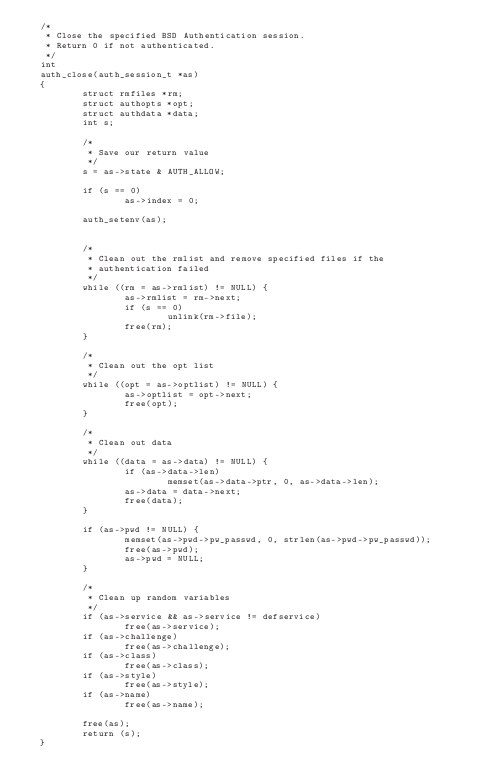
\includegraphics[width=1.0\linewidth, height=5cm]{source-code-img.png}

\caption{Zoomed Code}
\label{fig:zoomed}
\end{minipage}
\quad
\begin{minipage}[b]{0.55\linewidth}
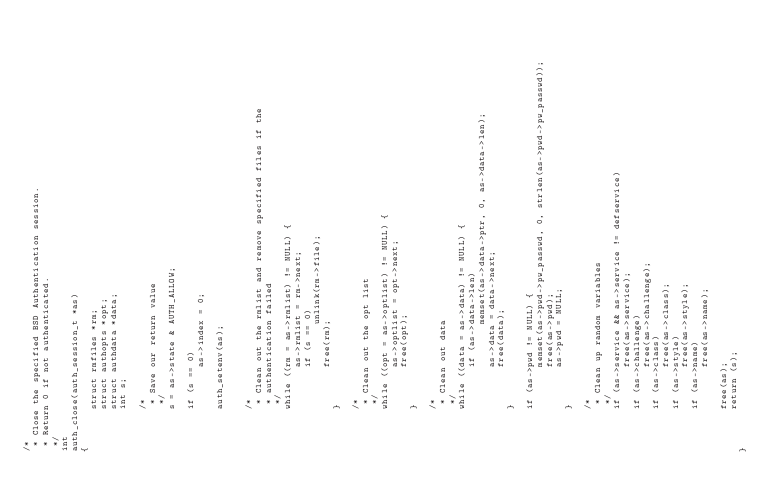
\includegraphics[width=1.0\linewidth, height=5cm]{source-code-img-sideways.png}

\caption{Rotated Code
\newline
Rotated code defines a time series with the value at time index $i$ equal to the length of line $i$.
}
\label{fig:rotated}
\end{minipage}
\end{figure}


In this approach we look at the shape of the code.   We use the line lengths (shown in figure \ref{fig:rotated})  as they exist in the source code to create a time series .  We include comments, indentation, blank lines and other potentially skewing portions of a source code file.  The details of the approaches taken are discussed in section \ref{DetailsExtractions}.  These extractions are chosen because we want to preserve the structure as a programmer would encounter it.  We do not want to analyze the program as the system would encounter it (e.g. after compilation, as would be used in static or dynamic analysis, see section \ref{RelatedWork} for more information).  

%TODO why is the cumulative sum taken?
Once we have a time series, we obtain the cumulative sum (by removing the mean values, because this allows long term persistence trends to be measured, this technique is typical for this type of analysis \cite{Suteanu:ArticWind:14, Suteanu:AirTemps:14}).  These are shown in the graphs in section \ref{DetailsResults} and Appendices \ref{FullResults} \& \ref{FullResultsOther}.  On these, we perform an analysis to see how space filling the curve is, and plot it on a dual logarithmic scale to compare it to an expected power law relationship (as performed in \cite{Kantelhardt:DFA:01}, \cite{Suteanu:AirTemps:14}, and \cite{Suteanu:ArticWind:14}).  To do this we use "detrended flucuation analysis" (DFA) as described in \cite{Kantelhardt:DFA:01} and detailed in section \ref{DetailsAnalyses}.  We choose this because of the detrending features of the analysis (detrending means to remove localized trends), allowing us to analyze the file as a whole, removing trends local to individual functions.  


The analysis gives us an exponent $H$, the "H Value", a variability and confidence level $R$ that the fluctuation value $F(s)$ relates to $s$ (the source line number).  These values are summarized in section \ref{DetailsResults} and the meaning \& derivation of the "H value" are given in section \ref{DFAHValue} .  

%TODO H-value should be defined or forward reference to the next TODO

\section{The Details}
We obtain the results in section \ref{DetailsResults} using the process described in this section.  A summary of the full data sets is in appendices \ref{FullResults} and \ref{FullResultsOther}.  The selection criteria for data set selection is in section \ref{DetailsCorpora}.

According to the work by Radjenovic in his survey of software metrics \cite{Radjenovic:SoftwareMetrics:13}, past metrics have been tested against varying size codebases.  In the survey a small codebase to test on would encompass less than 50,000 lines of code, and a large codebase would be more than 250,000.  We examine approximately 80,000 lines, a reasonable corpus by the standards of the survey.

The remainder of this section details the processes used to obtain the result tables and plots shown in the appendices.
\subsection{Corpora}\label{DetailsCorpora}

%TODO footnote openbsd
The selected C source code all comes from the OpenBSD system.  The rationale for selecting this system is that it is a small project (small team), it is mostly built in the same language, it is open source (and thus the source is available), the source covers user applications (like bash), compilers (like gcc), devices (like pci network devices) and network services like the nginx web service.

The selection criteria are summarized as follows:
\begin{itemize}
\item openbsd is focused on security and code quality;
\item single codebase all bundled together;
\item single language all chosen files are written in C;
\item length: all files are between 3500 and 3600 lines of code.;
\item broad source types: compilers, device drivers, utilities, network services.
\end{itemize}

We additionally analyze source code from Ruby, C\#, Java, HTML and Javascript projects (results in appendix \ref{FullResultsOther}), as evidence of the claim of language independence.  The interpretation in section \ref{DetailsInterpretation} is based largely on the C source from OpenBSD however (to avoid clouding the issue with too many apples versus oranges comparisons).

\subsection{Extractions}\label{DetailsExtractions}
We extract the time series by simply measuring the length of each line.  Consider the simple program in figure \ref{fig:ExampleCode}.  This program would yield the time series in figure \ref{fig:ExampleTimeSeries}.

\begin{figure}[h]
\centering
\begin{minipage}[b]{0.45\linewidth}
\begin{lstlisting}[frame=single]
int main(void) {
	return 0;
}
\end{lstlisting}

\caption{Example Code}
\label{fig:ExampleCode}
\end{minipage}
\quad
\begin{minipage}[b]{0.45\linewidth}
\begin{center}

\begin{quote}
1, 17 \\
2, 18 \\
3, 2
\end{quote}
\end{center}

\caption{Example Time Series}
\label{fig:ExampleTimeSeries}
\end{minipage}
\end{figure}

The values denote the line number followed by the number of characters on the line.  The last value "$3,2$" may be surprising, but the line contains the invisible end-of-file character.  Likewise, the other lines contain the invisible newline character, adding 1 to their character count.  Another possibly surprising value is that line 2 has 18 characters.  In this case, the indentation is composed of space characters.  Sometimes these are tab characters, which can be expanded to varying sizes depending on the settings of the editor being used to view the code.

Due to this variability, the extractions are performed with 4 configurations:
\begin{itemize}
\item \textbf{Naive}: the whole source file is processed as it is stated.   Tab characters, leading and trailing spaces, and other non-printed characters are left intact.
\item \textbf{Tab3}: tab characters are expanded to a fixed size of three blank spaces.
\item \textbf{Tab8}: tab characters are expanded to a fixed size of eight blank spaces.
\item \textbf{Trim}: all "whitespace" characters, including both tab characters and blank spaces are stripped from the beginning and end of each line.
\end{itemize}

The "Naive" configuration is justified by the fact that the unedited source code is precisely the artifact encountered by developers during maintenance or modification.  The tab-expanding configurations "Tab3" and "Tab8" are performed to examine the impact of changing tab expansion settings (which can be configured by users in their editors or IDEs).  Finally, the "Trim" configuration is used to completely remove whitespace, and thus examine purely the textual information content of each line.  The variance induced in the measurements (described in section \ref{DetailsAnalyses}) can be found in appendices \ref{FullResultsVariance} and \ref{FullResultsOtherVariance}.  A discussion of the impact of these choices is given in section \ref{DetailsResultsVariance}.

%TODO describe the time series for the sample program if it was tabs under the 4 configs.

\subsection{Analyses}\label{DetailsAnalyses}


We use the method for detrending fluctuation analysis described in detail by Kantelhardt in \cite{Kantelhardt:DFA:01} using a matlab implementation developed by Suteanu for use in his analysis of wind and temperature patterns in \cite{Suteanu:AirTemps:14} and \cite{Suteanu:ArticWind:14}. 

The four configurations described in the previous section (\ref{DetailsExtractions}) each yield a time series.  

We transform the time series into a cumulative sum, by calculating the average "height" of the time series, and subtracting it from each point.  These graphs are shown in appendices \ref{FullResults} and \ref{FullResultsOther}, and selected results highlighted in section \ref{DetailsResultsGraphs}.  

%TODO need to check this description with Dr. S.
Next the results are "detrended".  In the Kantelhardt paper, the detrending is always performed according to an "order", which defines the degree of the polynomial we fit to each segment.  This is done by repeatedly building a sliding segment, and find a best-fit polynomial to the points in the segment.  The series of polynomials according to the segments are then connected into a single composite function.  The function $F(s)$ associates the fluctuation with the scale $s$.  The precise details are in \cite{Kantelhardt:DFA:01} and the source code is in appendix \ref{SourceCodeMatlab}.  This function is then plotted on a logarithmic scale (on both the scale axis and the fluctuation axis), the full set of plots is available in appendices \ref{FullResults} and \ref{FullResultsOther}, and selected exemplars are given in section \ref{DetailsResults}.

Finally, a linear regression is performed to find the "H-value"\footnote{Note in the DFA world this value is different from other fractal dimension H-values, named by Mandelbrot in honor of Harold  Hurst} (the slope of the curve on the log-log scale), the confidence interval and "R-value" for each fluctuation versus scale plot.  The results are given in full the table in appendices \ref{FullResults} and \ref{FullResultsOther}, and their implications are discussed in section \ref{DetailsInterpretation}.

\label{DFAHValue}
The H-Value is derived as follows.  If we take $U(i)$ to be the time series data obtained from the rotated source code (normalized by subtracting the average line length), then we can take the cumulative sum $Q(i) = \sum\limits_{j=1}^i U(j)$.  For each segment $m$ of the sum, we denote the weighted average $w_{s,m} = Q_m(i) - P_{m,N}(i)$, where $P_{m,N}$ denotes the best-fit polynomial of degree $N$ for the segment $m$.  In this analysis $N$ is always 2 (that is, we use the best fitting quadratic).  From here the weighted average is taken, removing any negative values: $F^2_s(m) = <w^2_{s,m}(i)>$.  For each of the $r$ segments of length $s$ we obtain $F(s) = [ r^{-1} \sum\limits_{m=1}^r F^2_s(m)]^{1/2}$.  If this fluctuation function $F$ is proportional to the segment size $s$ per $F^N(s) \propto S^H$, then:

\begin{quote}
[T]he exponent $H$ characterizes the long-range correlations over the scale range spanned by
$s$ for which this power law is valid. [...] If $H > 0.5$, the pattern is
persistent, i.e., increases (decreases) in the time series tend to be followed by further
increases (decreases). \cite{Suteanu:AirTemps:14}
\end{quote}

Readers interested in the exact details of DFA analysis can consult \cite{Suteanu:AirTemps:14}, \cite{Kantelhardt:DFA:01}, or view the Matlab source code used in Appendix \ref{SourceCodeMatlab}.
%TODO the forward referencing is a little repetitive, worth using?
%TODO define H value in detail here w/ appropriate citation

\section{Results}\label{DetailsResults}

Following the procedure in sections \ref{DetailsExtractions} and \ref{DetailsAnalyses}, we find that some files give a strong long-term scaling pattern, others lack long-term scaling, and some give poor results from this type of analysis.

The full analysis table is given in Appendices \ref{FullResults}, \ref{FullResultsOther} and \ref{FullResultsBenchmarks}.  The H-values range from 0.56351 (xilinx, naive) to 0.83862 (rcparse, naive), with confidence intervals ranging from 0.0056327 (recog, tab3) to 0.052436 (rcparse, naive), and R-Values between (rcparse, naive) and 0.99974 (recog, tab3).

\subsubsection{Table - DFA2 Analysis results per source file}
\begin{longtable}{l l r r r}
\textbf{Filename} & \textbf{Type} & \textbf{H} & \textbf{+/-} & \textbf{R} \\

{gnu/usr.bin/gcc/gcc/recog} & tab3 & 0.59492 & 0.0056327 & 0.99974 \\
{gnu/usr.bin/perl/hv} & tab8 & 0.70414 & 0.008119 & 0.99961 \\
{gnu/usr.bin/binutils/binutils/rcparse} & naive & 0.83862 & 0.052436 & 0.98867 \\



\end{longtable}

The first two results exhibit a strong R-value (correlation coefficient), with minimal confidence intervals, yet quite different H-values (implying a different persistence of long term scaling).

It is interesting to note that some of the outliers in the OpenBSD corpus correspond to source files automatically generated by parser-generators like Lex and Yacc. %TODO footnote these?


\subsubsection{Table - DFA2 Variability}\label{DetailsResultsVariance}
We observe the variance of the H-value, confidence interval and R-value across each of the four configurations.  The maximal variability for each value is shown below.

\begin{longtable}{l r}
\textbf{Filename} &  \textbf{H} \\

{usr.sbin/bgpd/rde} & 0.16517000000000004  \\
\end{longtable}
This shows the "rde" file exhibits quite a substantial variation of observed H-values, and the highest observed variation.  See appendix \ref{FullResultsVariance} for full table. 
\begin{longtable}{l l r r r}
\textbf{Filename} & \textbf{Type} & \textbf{H} & \textbf{+/-} & \textbf{R} \\

{usr.sbin/bgpd/rde} & naive & 0.61891 & 0.0097795 & 0.99927 \\
{usr.sbin/bgpd/rde} & trim & 0.59715 & 0.0099081 & 0.99919 \\
{usr.sbin/bgpd/rde} & tab3 & 0.66746 & 0.013262 & 0.99884 \\
{usr.sbin/bgpd/rde} & tab8 & 0.76232 & 0.016056 & 0.9987 \\
\end{longtable}
We see values ranging from 0.59715 in the "trim" configuration, to 0.76232 in the "tab8" configuration (recall this means that tab characters are expanded to 8 characters).


\begin{longtable}{l r}
\textbf{Filename} &  \textbf{+/-} \\
{sys/dev/pci/if/oce} & 0.024596999999999997  \\
\end{longtable}
This shows the "oce" file has a variance of roughly 0.0246 in the confidence interval.

\begin{longtable}{l l r r r}
\textbf{Filename} & \textbf{Type} & \textbf{H} & \textbf{+/-} & \textbf{R} \\
{sys/dev/pci/if/oce} & tab8 & 0.65203 & 0.014539 & 0.99854 \\
{sys/dev/pci/if/oce} & tab3 & 0.65598 & 0.028076 & 0.99465 \\
{sys/dev/pci/if/oce} & naive & 0.67102 & 0.036174 & 0.99154 \\
{sys/dev/pci/if/oce} & trim & 0.67623 & 0.039136 & 0.99027 \\
\end{longtable}
The values range from +/- 0.0145 to +/- 0.039, for the "tab8" and "trim" configurations respectively.

\begin{longtable}{l r}
\textbf{Filename} &  \textbf{R} \\
{gnu/gcc/gcc/config/cris/cris} & 0.005229999999999957  \\
\end{longtable}
Turning to the R-value, we find that the maximal variance is only about 0.005, which suggests the correlation of the fluctuation and the scale of the analysis (between 10 to 1100 lines) is not significantly impacted by the choice of tab expansion or whitespace trimming.



\subsubsection{Graphs}\label{DetailsResultsGraphs}
\begin{center}
\includegraphics[width=1.0\linewidth, height=5cm]{{gnu_usr.bin_gcc_gcc_recog_c_tab3_time_series}.png}
\includegraphics[width=1.0\linewidth, height=5cm]{{gnu_usr.bin_gcc_gcc_recog_c_tab3_log_log}.png}
\end{center}
This shows a high correlation coefficient, corresponding to a mild long-term persistence.
\begin{center}
\includegraphics[width=1.0\linewidth, height=5cm]{{gnu_usr.bin_perl_hv_c_tab8_time_series}.png}
\includegraphics[width=1.0\linewidth, height=5cm]{{gnu_usr.bin_perl_hv_c_tab8_log_log}.png}
\end{center}

This shows a high correlation coefficient, corresponding to a more substantial long term persistence.
\begin{center}
\includegraphics[width=1.0\linewidth, height=5cm]{{gnu_usr.bin_binutils_binutils_rcparse_c_naive_time_series}.png}
\includegraphics[width=1.0\linewidth, height=5cm]{{gnu_usr.bin_binutils_binutils_rcparse_c_naive_log_log}.png}
\end{center}

This shows an example of poor correlation coefficient, suggesting the linear curve fit is not entirely accurate.


\subsection{Interpretation}\label{DetailsInterpretation}

The three cases shown in section \ref{DetailsResults}, tells us about the long term persistence of the fluctuation.  In order to provide meaningful comparisons between observed H-values, we focus our studies on the source code files which yield confidence intervals strictly better than 0.02.  This leaves us with about half of the sources for study\footnote{ "gnu/usr.bin/gcc/gcc/recog.c",
"gnu/gcc/gcc/recog.c",
"gnu/usr.bin/perl/hv.c",
"usr.sbin/bgpd/rde.c",
"sys/dev/audio.c",
"gnu/gcc/gcc/config/cris/cris.c",
"gnu/usr.bin/
gcc/gcc/config/mcore/mcore.c",
"gnu/gcc/gcc/dbxout.c",
"gnu/usr.bin/gcc/gcc/java/expr.c",
"sys/dev/ic/mpi.c",
"sys/dev/pci/if-san-xilinx.c", and
"sys/arch/arm/arm/pmap7.c"}.

Restricted thusly, we find the H-values range between 0.58113 for "gnu/gcc/gcc/config/cris/cris.c" and 0.69928 for "gnu/usr.bin/perl/hv.c".

In order to provide an interpretation of the range of values observed we examine the source files directly and find the following observations of high H-value source files:

\begin{itemize}
\item many make extensive use of macros, which in some cases flatten looping and conditional constructs;
\item many make use of strict formatting guidelines, such as line limiting to 80 columns (a standard terminal width);
\item relatively large numbers of shorter functions;
\item limited nesting of constructs;
\item limited usage of preprocessor directives (outside of macro expansions), specifically: few calls to "\#ifdef" and related expansions;
\item detailed comments in full paragraph form (as opposed to terse notes)
\item lines manually and explicitly lengthened by using backslashes as a line continuation character in C, repeated space or tab characters to align variable declarations.
\end{itemize}

On the other hand, when we examine source files with a low H-value we find:
\begin{itemize}
\item frequent usage of boolean connectives (such as "||" for OR, "\&\&" for AND, etc);
\item frequent usage of bitwise operators (such as "<<" for shifting, etc);
\item frequent use of the case/switch operator.

\end{itemize}

Interestingly, the lower the H-value, the higher the long term persistence is to be expected.

In summary:
\begin{itemize}
\item complexity, how likely is it that another block of code will not look like the current one.
\item scaling, how likely is it that the module will have the same jaggedness if you look at larger and larger blocks.
\end{itemize}

\section{Related Work}\label{RelatedWork}

The most well-known software complexity metric is due to McCabe \cite{McCabe:SoftwareComplexity:76}.
Looking at the C source files with a confidence interval below 0.02, we find no correlation between H-values and averaged McCabe complexity.  This suggests the fractal dimension of a text source is not directly related to the number of paths through the code (i.e. the number of conditional statements or loops is not the determining factor).  A summary of the averaged McCabe values along with H-values is given in appendix \ref{McCabeAveraged}.


Per the discussion in the comprehensive survey \cite{Radjenovic:SoftwareMetrics:13} by Radjenovic many software quality metrics focus on connectivity in an object-oriented sense.  That is to say they frequently rely on measuring coupling between components by virtue of inheritance, polymorphism, composition of objects, implementation of interfaces and other aspects of software design that only apply to object oriented programming.  These approaches rule out evaluation of procedural (such as C), or functional (such as Haskell) languages. 


Other metrics like McCabe's cyclomatic complexity focus on branching and looping (to determine paths through the code).  These are more general and apply well to both procedural and object oriented code.  However they fall flat in handling non-imperative languages, including functional languages like Haskell or declarative goal-driven languages like Prolog.   It is also worth noting that cyclomatic complexity is an unbounded/non-normalized measure.  This makes it difficult to compare source files as a whole, as it really measures the individual functions - longer files are much more likely to report a higher overall complexity.  Taking the average across all the functions gives a semi-normalized value, but it is still not strictly bounded.


There have been past efforts to use fractal dimension metrics to quantify software systems, most notably \cite{Concas:FractalSoftware:06} and \cite{Valverde:SmallWorlds:03}.  However both of these systems require object oriented programming languages as they operate on the graph implicit in the connections and coupling between components.  Concas' work makes use of the "box counting" method of fractal analysis, which is not intended to remove localized trends in the shape of the fractal.

The metrics identified by Radjenovic's survey and the fractal based metrics by Concas and Valverde all compare source code written in the same source language.  Our approach is capable of comparing program sources written in different languages.

% TODO static/dynamic analysis?


\section{Conclusion and Future Work}

The scaling results we have found in this work suggest an interesting source of new knowledge is available with this line of research.  Some examples of future work might include:
\begin{itemize}
\item Examining the same algorithm implemented in multiple languages/across paradigms (functional vs OO vs procedural etc).  The implementations would need to be considered idiomatic to the language to be meaningful.
\item Examining a similar type of project in different languages (e.g. DB driven web application in python/django, ruby/rails, C\#/MVC).
\item Examining similar type of program in the same language (e.g. redhat linux vs debian linux versus openbsd versus freebsd, etc).
\item Comparing tested projects to untested (projects with a thorough test suite vs ones that are not automatically tested).
\item Comparing projects considered good or bad according to other software quality metrics (perhaps according to existing metrics or by evaluation by professional programmers, e.g. works considered "beautiful" \cite{Wilson:BeautifulCode:07})
\end{itemize}

In summary, this approach permits cross-language comparisons, it makes no assumptions about the paradigm of the languages being evaluated; it requires no knowledge of the semantic content of the source; it is normalized and bounded; and it takes into account all the text items encountered by real-world maintainers (indentation, comments, long or short variable names).  

One the other hand, our approach is truly unaware of semantic structure of the source.  It is also weaker because of inconsistent applicability, including certain files that simply show no persistent scaling properties, whether strong or weak; and because interpretation of the nature of the complexity being measured is challenging.

\subsection{Acknowledgments}
I would like to thank Dr. Cristian Suteanu for both sparking this idea during a lecture on pattern analysis and for being extremely generous with his time afterwards to help develop the ideas contained here, the Matlab code to perform the DFA analysis, and for helping me understand how to interpret the results.
I would also like to thank Dr. Konstantinidis for spurring on this research idea.
\newpage
\bibliographystyle{acm}
\bibliography{research}

\newpage
%\begin{appendices}
%\section{Full Results - C}\label{FullResults}
%
\subsection{Table - DFA2 Analysis results per source file}
\begin{longtable}{l l r r r}
\textbf{Filename} & \textbf{Type} & \textbf{H} & \textbf{+/-} & \textbf{R} \\
{gnu/usr.bin/gcc/gcc/recog} & tab3 & 0.59492 & 0.0056327 & 0.99974 \\
{gnu/gcc/gcc/dbxout} & trim & 0.59263 & 0.0061208 & 0.99969 \\
{gnu/usr.bin/perl/hv} & tab8 & 0.70414 & 0.008119 & 0.99961 \\
{gnu/gcc/gcc/dbxout} & tab3 & 0.60669 & 0.0069868 & 0.99961 \\
{gnu/usr.bin/gcc/gcc/recog} & tab8 & 0.6277 & 0.0072911 & 0.9996 \\
{gnu/gcc/gcc/dbxout} & naive & 0.59439 & 0.0069626 & 0.9996 \\
{gnu/usr.bin/gcc/gcc/recog} & trim & 0.58905 & 0.0073385 & 0.99954 \\
{sys/dev/ic/mpi} & tab8 & 0.63435 & 0.0079974 & 0.99953 \\
{sys/dev/ic/mpi} & tab3 & 0.65327 & 0.0082775 & 0.99953 \\
{gnu/gcc/gcc/recog} & trim & 0.59532 & 0.0075579 & 0.99953 \\
{gnu/usr.bin/gcc/gcc/recog} & naive & 0.5966 & 0.0079926 & 0.99947 \\
{gnu/usr.bin/perl/hv} & tab3 & 0.69224 & 0.0097339 & 0.99942 \\
{sys/dev/pci/if/san/xilinx} & tab3 & 0.59175 & 0.0087195 & 0.99936 \\
{usr.sbin/bgpd/rde} & naive & 0.61891 & 0.0097795 & 0.99927 \\
{gnu/usr.bin/gcc/gcc/java/expr} & tab3 & 0.63189 & 0.010224 & 0.99923 \\
{usr.sbin/bgpd/rde} & trim & 0.59715 & 0.0099081 & 0.99919 \\
{sys/dev/ic/mpi} & naive & 0.66608 & 0.011323 & 0.99915 \\
{gnu/gcc/gcc/recog} & naive & 0.59523 & 0.010179 & 0.99914 \\
{sys/dev/audio} & tab3 & 0.59244 & 0.010359 & 0.9991 \\
{sys/dev/pci/if/san/xilinx} & naive & 0.56351 & 0.0098886 & 0.99909 \\
{gnu/usr.bin/perl/hv} & naive & 0.69928 & 0.012633 & 0.99904 \\
{sys/dev/ic/mpi} & trim & 0.65627 & 0.011851 & 0.99904 \\
{gnu/usr.bin/gcc/gcc/java/expr} & naive & 0.62566 & 0.01174 & 0.99896 \\
{sys/dev/audio} & tab8 & 0.64505 & 0.012165 & 0.99895 \\
{gnu/gcc/gcc/recog} & tab3 & 0.58913 & 0.011115 & 0.99895 \\
{sys/dev/pci/if/san/xilinx} & trim & 0.56666 & 0.010914 & 0.99891 \\
{gnu/gcc/gcc/dbxout} & tab8 & 0.66126 & 0.01297 & 0.99887 \\
{sys/dev/audio} & trim & 0.58605 & 0.011504 & 0.99887 \\
{sys/arch/arm/arm/pmap7} & tab8 & 0.66145 & 0.013067 & 0.99885 \\
{usr.sbin/bgpd/rde} & tab3 & 0.66746 & 0.013262 & 0.99884 \\
{gnu/usr.bin/gcc/gcc/java/expr} & tab8 & 0.65126 & 0.013331 & 0.99877 \\
{gnu/usr.bin/gcc/gcc/config/mcore/mcore} & trim & 0.66775 & 0.013741 & 0.99875 \\
{gnu/usr.bin/gcc/gcc/config/mcore/mcore} & naive & 0.67327 & 0.013939 & 0.99874 \\
{usr.sbin/bgpd/rde} & tab8 & 0.76232 & 0.016056 & 0.9987 \\
{gnu/usr.bin/gcc/gcc/config/mcore/mcore} & tab3 & 0.67179 & 0.014159 & 0.99869 \\
{gnu/gcc/gcc/config/cris/cris} & trim & 0.58868 & 0.012673 & 0.99864 \\
{sys/dev/audio} & naive & 0.58739 & 0.012703 & 0.99862 \\
{gnu/gcc/gcc/recog} & tab8 & 0.619 & 0.013698 & 0.99856 \\
{gnu/usr.bin/perl/hv} & trim & 0.67169 & 0.014941 & 0.99855 \\
{sys/dev/pci/if/oce} & tab8 & 0.65203 & 0.014539 & 0.99854 \\
{gnu/usr.bin/gcc/gcc/config/mcore/mcore} & tab8 & 0.68192 & 0.015549 & 0.99847 \\
{gnu/usr.bin/binutils-2.17/binutils/dlltool} & tab8 & 0.70437 & 0.016121 & 0.99846 \\
{gnu/usr.bin/gcc/gcc/java/expr} & trim & 0.6216 & 0.014288 & 0.99845 \\
{sys/dev/pci/if/san/xilinx} & tab8 & 0.69829 & 0.016051 & 0.99845 \\
{gnu/usr.bin/gcc/gcc/config/d30v/d30v} & tab8 & 0.6478 & 0.016048 & 0.9982 \\
{sys/arch/arm/arm/pmap7} & tab3 & 0.60489 & 0.01537 & 0.9981 \\
{gnu/usr.bin/binutils-2.17/binutils/dlltool} & tab3 & 0.67957 & 0.019866 & 0.99749 \\
{lib/libpcap/gencode} & trim & 0.68244 & 0.021502 & 0.99709 \\
{lib/libpcap/gencode} & naive & 0.68849 & 0.021903 & 0.99703 \\
{gnu/usr.bin/binutils-2.17/binutils/dlltool} & naive & 0.67264 & 0.021469 & 0.99701 \\
{gnu/gcc/gcc/config/cris/cris} & naive & 0.58113 & 0.018732 & 0.99695 \\
{lib/libpcap/gencode} & tab3 & 0.70019 & 0.022772 & 0.9969 \\
{sys/arch/arm/arm/pmap7} & trim & 0.59658 & 0.019706 & 0.9968 \\
{sys/arch/arm/arm/pmap7} & naive & 0.5988 & 0.019811 & 0.99679 \\
{gnu/usr.bin/binutils-2.17/bfd/elf32-s390} & naive & 0.73052 & 0.02483 & 0.99661 \\
{gnu/usr.bin/binutils-2.17/bfd/elf32-s390} & trim & 0.73983 & 0.0262 & 0.99632 \\
{lib/libpcap/gencode} & tab8 & 0.74311 & 0.026836 & 0.99618 \\
{gnu/usr.bin/binutils-2.17/bfd/elf32-s390} & tab3 & 0.73373 & 0.026766 & 0.9961 \\
{gnu/usr.bin/binutils-2.17/opcodes/xc16x-desc} & trim & 0.82248 & 0.030216 & 0.99605 \\
{gnu/usr.bin/binutils-2.17/opcodes/xc16x-desc} & naive & 0.80899 & 0.029991 & 0.99597 \\
{gnu/usr.bin/binutils-2.17/opcodes/xc16x-desc} & tab3 & 0.80899 & 0.029991 & 0.99597 \\
{gnu/usr.bin/binutils-2.17/opcodes/xc16x-desc} & tab8 & 0.80899 & 0.029991 & 0.99597 \\
{gnu/usr.bin/binutils-2.17/binutils/dlltool} & trim & 0.67617 & 0.0254 & 0.99587 \\
{gnu/usr.bin/binutils/gas/config/tc-sh64} & trim & 0.6629 & 0.024982 & 0.99584 \\
{sys/dev/isa/gus} & tab8 & 0.74148 & 0.028409 & 0.9957 \\
{gnu/usr.bin/binutils-2.17/gas/config/tc-sh64} & trim & 0.66133 & 0.025382 & 0.99569 \\
{gnu/gcc/gcc/config/cris/cris} & tab3 & 0.5934 & 0.023363 & 0.99546 \\
{gnu/usr.bin/binutils-2.17/bfd/elf32-s390} & tab8 & 0.75431 & 0.031066 & 0.99504 \\
{usr.sbin/nginx/src/http/modules/module} & naive & 0.63568 & 0.026926 & 0.99475 \\
{usr.sbin/nginx/src/http/modules/module} & tab3 & 0.63568 & 0.026926 & 0.99475 \\
{usr.sbin/nginx/src/http/modules/module} & tab8 & 0.63568 & 0.026926 & 0.99475 \\
{gnu/usr.bin/binutils/gas/config/tc-sh64} & naive & 0.66906 & 0.028396 & 0.99473 \\
{gnu/usr.bin/binutils/gas/config/tc-sh64} & tab8 & 0.74488 & 0.031736 & 0.99469 \\
{sys/dev/pci/if/oce} & tab3 & 0.65598 & 0.028076 & 0.99465 \\
{gnu/usr.bin/binutils-2.17/gas/config/tc-sh64} & naive & 0.66763 & 0.028806 & 0.99456 \\
{gnu/usr.bin/binutils-2.17/gas/config/tc-sh64} & tab8 & 0.74279 & 0.032291 & 0.99448 \\
{gnu/usr.bin/gcc/gcc/config/d30v/d30v} & tab3 & 0.60473 & 0.026897 & 0.99422 \\
{gnu/usr.bin/binutils/binutils/rcparse} & tab8 & 0.80088 & 0.035676 & 0.9942 \\
{gnu/usr.bin/binutils/gas/config/tc-sh64} & tab3 & 0.68449 & 0.031632 & 0.99377 \\
{gnu/gcc/gcc/cp/decl2} & tab8 & 0.65354 & 0.030368 & 0.9937 \\
{gnu/usr.bin/binutils-2.17/gas/config/tc-sh64} & tab3 & 0.68297 & 0.032151 & 0.99353 \\
{gnu/gcc/gcc/config/cris/cris} & tab8 & 0.64966 & 0.030884 & 0.99341 \\
{sys/dev/isa/gus} & tab3 & 0.71938 & 0.034781 & 0.99318 \\
{gnu/usr.bin/gcc/gcc/config/d30v/d30v} & trim & 0.62112 & 0.030845 & 0.99281 \\
{gnu/gcc/gcc/cp/decl2} & naive & 0.63327 & 0.031792 & 0.99265 \\
{gnu/gcc/gcc/cp/decl2} & tab3 & 0.63641 & 0.032096 & 0.99259 \\
{gnu/gcc/gcc/cp/decl2} & trim & 0.63474 & 0.032774 & 0.99223 \\
{sys/dev/isa/gus} & naive & 0.71854 & 0.037617 & 0.99202 \\
{usr.sbin/nginx/src/http/modules/module} & trim & 0.6735 & 0.035662 & 0.99184 \\
{sys/dev/pci/if/oce} & naive & 0.67102 & 0.036174 & 0.99154 \\
{gnu/usr.bin/gcc/gcc/config/d30v/d30v} & naive & 0.60422 & 0.032721 & 0.99147 \\
{sys/dev/isa/gus} & trim & 0.71694 & 0.03908 & 0.99136 \\
{sys/dev/pci/if/oce} & trim & 0.67623 & 0.039136 & 0.99027 \\
{gnu/usr.bin/binutils/binutils/rcparse} & tab3 & 0.82709 & 0.048396 & 0.99006 \\
{gnu/usr.bin/binutils/binutils/rcparse} & trim & 0.82182 & 0.051147 & 0.98878 \\
{gnu/usr.bin/binutils/binutils/rcparse} & naive & 0.83862 & 0.052436 & 0.98867 \\
\end{longtable}

\newpage
\subsection{Table - DFA2 Variance}\label{FullResultsVariance}

\begin{longtable}{l r}
\textbf{Filename} &  \textbf{H} \\
{gnu/gcc/gcc/config/cris/cris} & 0.06852999999999998  \\
{gnu/gcc/gcc/cp/decl2} & 0.02027000000000001  \\
{gnu/gcc/gcc/dbxout} & 0.06862999999999997  \\
{gnu/gcc/gcc/recog} & 0.029869999999999952  \\
{gnu/usr.bin/binutils-2.17/bfd/elf32-s390} & 0.02379000000000009  \\
{gnu/usr.bin/binutils-2.17/binutils/dlltool} & 0.031730000000000036  \\
{gnu/usr.bin/binutils-2.17/gas/config/tc-sh64} & 0.08145999999999998  \\
{gnu/usr.bin/binutils-2.17/opcodes/xc16x-desc} & 0.013490000000000002  \\
{gnu/usr.bin/binutils/binutils/rcparse} & 0.037739999999999996  \\
{gnu/usr.bin/binutils/gas/config/tc-sh64} & 0.08197999999999994  \\
{gnu/usr.bin/gcc/gcc/config/d30v/d30v} & 0.04358000000000006  \\
{gnu/usr.bin/gcc/gcc/config/mcore/mcore} & 0.014170000000000016  \\
{gnu/usr.bin/gcc/gcc/java/expr} & 0.02965999999999991  \\
{gnu/usr.bin/gcc/gcc/recog} & 0.03865000000000007  \\
{gnu/usr.bin/perl/hv} & 0.03244999999999998  \\
{lib/libpcap/gencode} & 0.06067  \\
{sys/arch/arm/arm/pmap7} & 0.06486999999999998  \\
{sys/dev/audio} & 0.05900000000000005  \\
{sys/dev/ic/mpi} & 0.031730000000000036  \\
{sys/dev/isa/gus} & 0.024540000000000006  \\
{sys/dev/pci/if/oce} & 0.0242  \\
{sys/dev/pci/if/san/xilinx} & 0.13478  \\
{usr.sbin/bgpd/rde} & 0.16517000000000004  \\
{usr.sbin/nginx/src/http/modules/ngx/http/mp4/module} & 0.037819999999999965  \\
\end{longtable}
\begin{longtable}{l r}
\textbf{Filename} &  \textbf{+/-} \\
{gnu/gcc/gcc/config/cris/cris} & 0.018211  \\
{gnu/gcc/gcc/cp/decl2} & 0.0024059999999999984  \\
{gnu/gcc/gcc/dbxout} & 0.006849200000000001  \\
{gnu/gcc/gcc/recog} & 0.0061401  \\
{gnu/usr.bin/binutils-2.17/bfd/elf32-s390} & 0.0062359999999999985  \\
{gnu/usr.bin/binutils-2.17/binutils/dlltool} & 0.009278999999999999  \\
{gnu/usr.bin/binutils-2.17/gas/config/tc-sh64} & 0.006909000000000002  \\
{gnu/usr.bin/binutils-2.17/opcodes/xc16x-desc} & 0.0002249999999999995  \\
{gnu/usr.bin/binutils/binutils/rcparse} & 0.016760000000000004  \\
{gnu/usr.bin/binutils/gas/config/tc-sh64} & 0.006754  \\
{gnu/usr.bin/gcc/gcc/config/d30v/d30v} & 0.016673  \\
{gnu/usr.bin/gcc/gcc/config/mcore/mcore} & 0.0018080000000000006  \\
{gnu/usr.bin/gcc/gcc/java/expr} & 0.004064  \\
{gnu/usr.bin/gcc/gcc/recog} & 0.0023599000000000007  \\
{gnu/usr.bin/perl/hv} & 0.006822  \\
{lib/libpcap/gencode} & 0.0053339999999999985  \\
{sys/arch/arm/arm/pmap7} & 0.006743999999999998  \\
{sys/dev/audio} & 0.0023440000000000006  \\
{sys/dev/ic/mpi} & 0.0038536000000000004  \\
{sys/dev/isa/gus} & 0.010670999999999996  \\
{sys/dev/pci/if/oce} & 0.024596999999999997  \\
{sys/dev/pci/if/san/xilinx} & 0.0073314999999999995  \\
{usr.sbin/bgpd/rde} & 0.006276500000000001  \\
{usr.sbin/nginx/src/http/modules/ngx/http/mp4/module} & 0.008736  \\
\end{longtable}
\begin{longtable}{l r}
\textbf{Filename} &  \textbf{R} \\
{gnu/gcc/gcc/config/cris/cris} & 0.005229999999999957  \\
{gnu/gcc/gcc/cp/decl2} & 0.0014700000000000824  \\
{gnu/gcc/gcc/dbxout} & 0.0008199999999999319  \\
{gnu/gcc/gcc/recog} & 0.0009700000000000264  \\
{gnu/usr.bin/binutils-2.17/bfd/elf32-s390} & 0.0015699999999999603  \\
{gnu/usr.bin/binutils-2.17/binutils/dlltool} & 0.002589999999999981  \\
{gnu/usr.bin/binutils-2.17/gas/config/tc-sh64} & 0.0021599999999999397  \\
{gnu/usr.bin/binutils-2.17/opcodes/xc16x-desc} & 7.999999999996898e-05  \\
{gnu/usr.bin/binutils/binutils/rcparse} & 0.005529999999999924  \\
{gnu/usr.bin/binutils/gas/config/tc-sh64} & 0.0020699999999999052  \\
{gnu/usr.bin/gcc/gcc/config/d30v/d30v} & 0.006730000000000014  \\
{gnu/usr.bin/gcc/gcc/config/mcore/mcore} & 0.000280000000000058  \\
{gnu/usr.bin/gcc/gcc/java/expr} & 0.0007800000000000029  \\
{gnu/usr.bin/gcc/gcc/recog} & 0.00026999999999999247  \\
{gnu/usr.bin/perl/hv} & 0.0010599999999999499  \\
{lib/libpcap/gencode} & 0.0009100000000000774  \\
{sys/arch/arm/arm/pmap7} & 0.0020600000000000618  \\
{sys/dev/audio} & 0.00048000000000003595  \\
{sys/dev/ic/mpi} & 0.0004899999999999904  \\
{sys/dev/isa/gus} & 0.0043400000000000105  \\
{sys/dev/pci/if/oce} & 0.00827  \\
{sys/dev/pci/if/san/xilinx} & 0.0009100000000000774  \\
{usr.sbin/bgpd/rde} & 0.0005699999999999594  \\
{usr.sbin/nginx/src/http/modules/ngx/http/mp4/module} & 0.002909999999999968  \\
\end{longtable}

\newpage
\subsection{Graphs}
\begin{center}
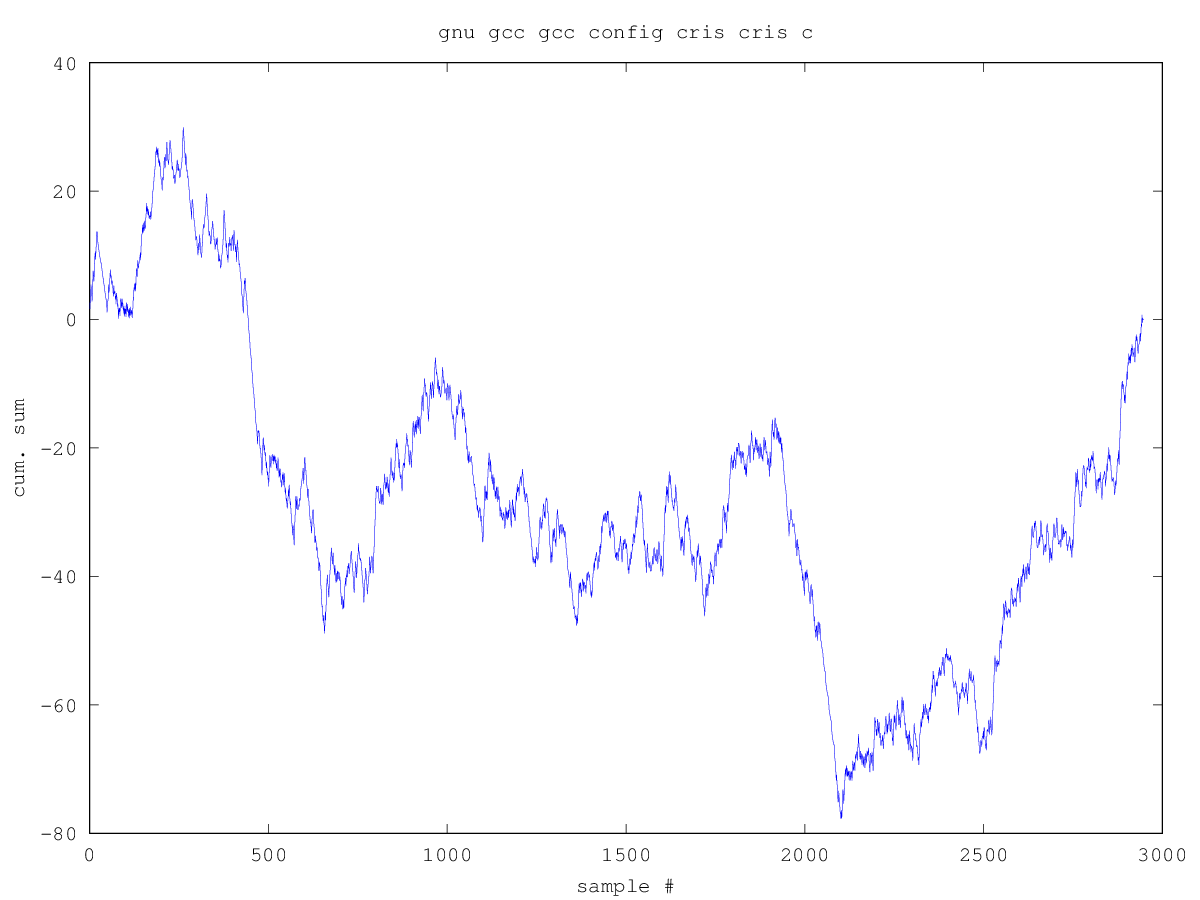
\includegraphics[width=0.8\linewidth]{{fractals/data/gnu_gcc_gcc_config_cris_cris_c_naive_time_series}.png}
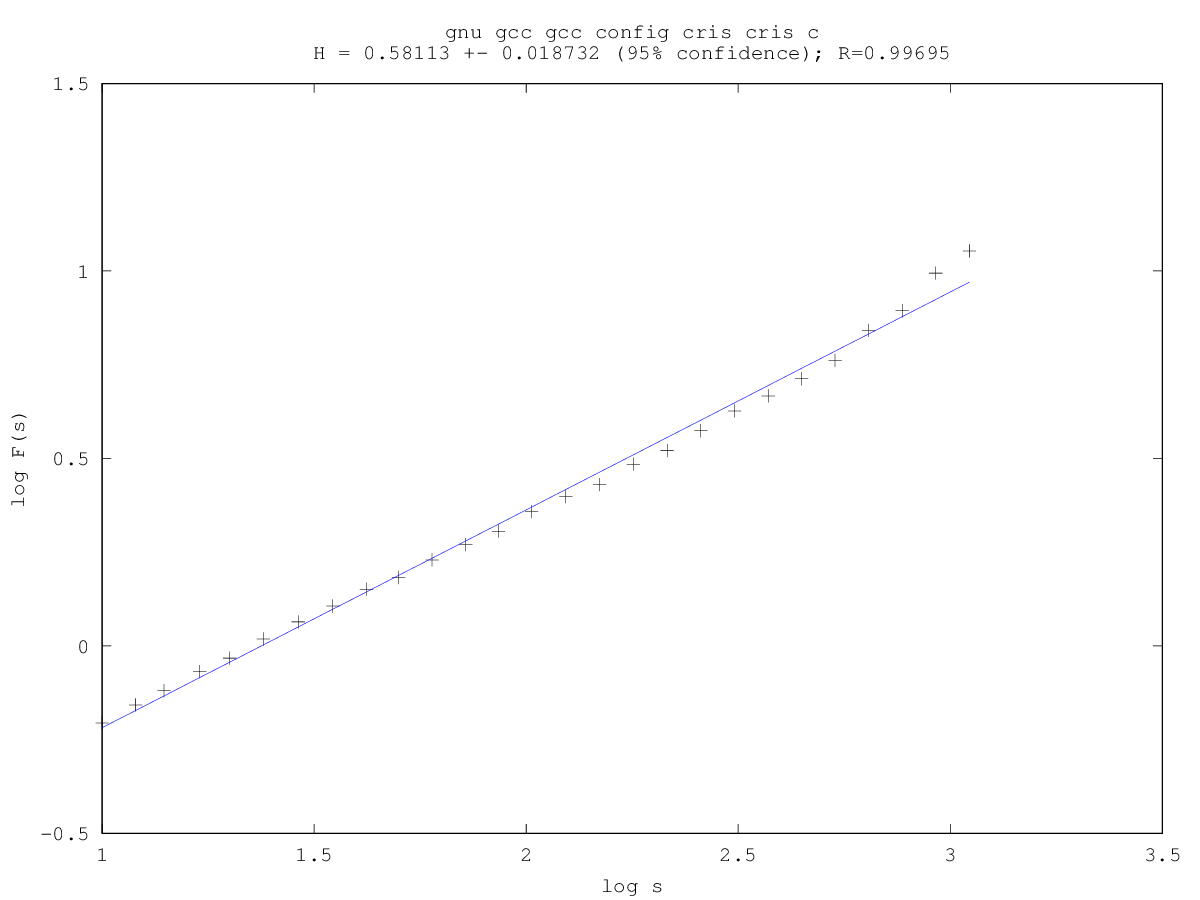
\includegraphics[width=0.8\linewidth]{{fractals/data/gnu_gcc_gcc_config_cris_cris_c_naive_log_log}.png}
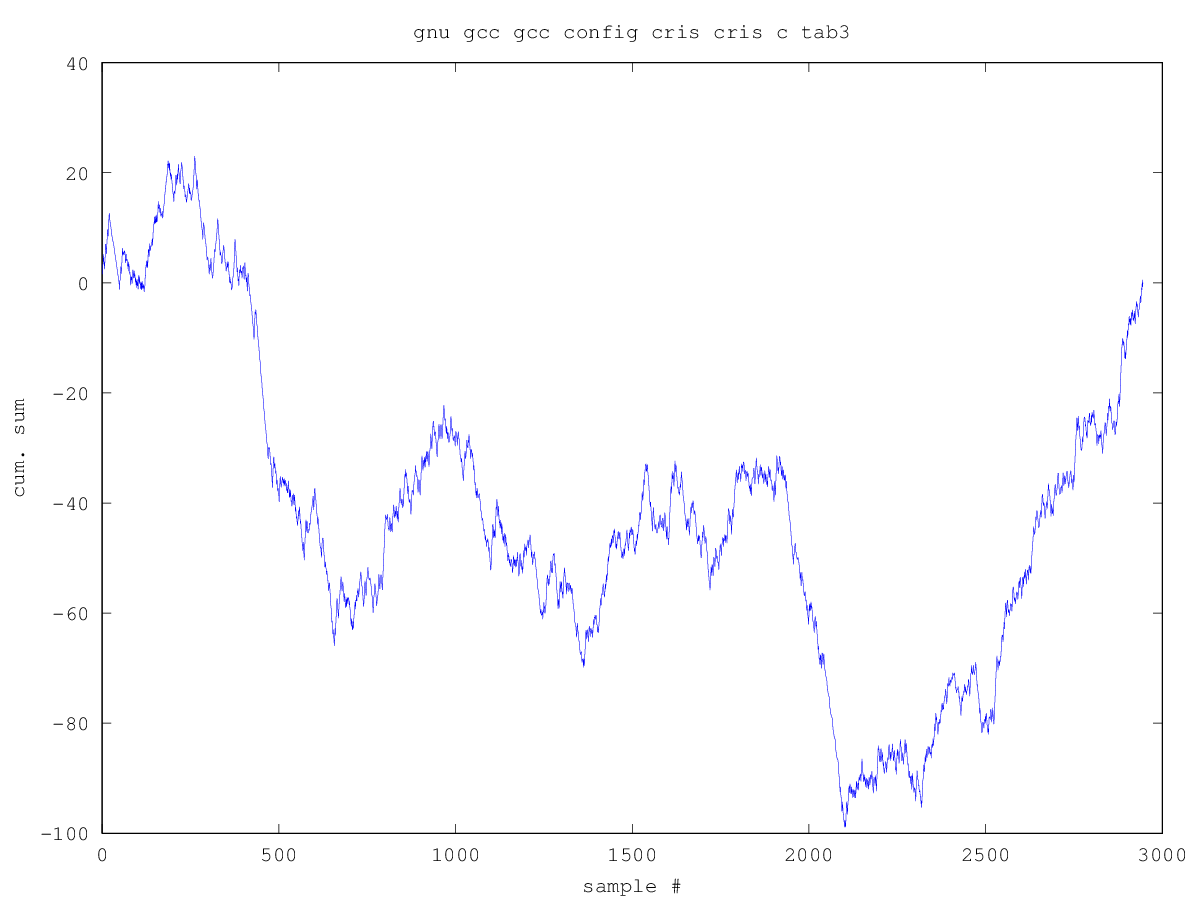
\includegraphics[width=0.8\linewidth]{{fractals/data/gnu_gcc_gcc_config_cris_cris_c_tab3_time_series}.png}
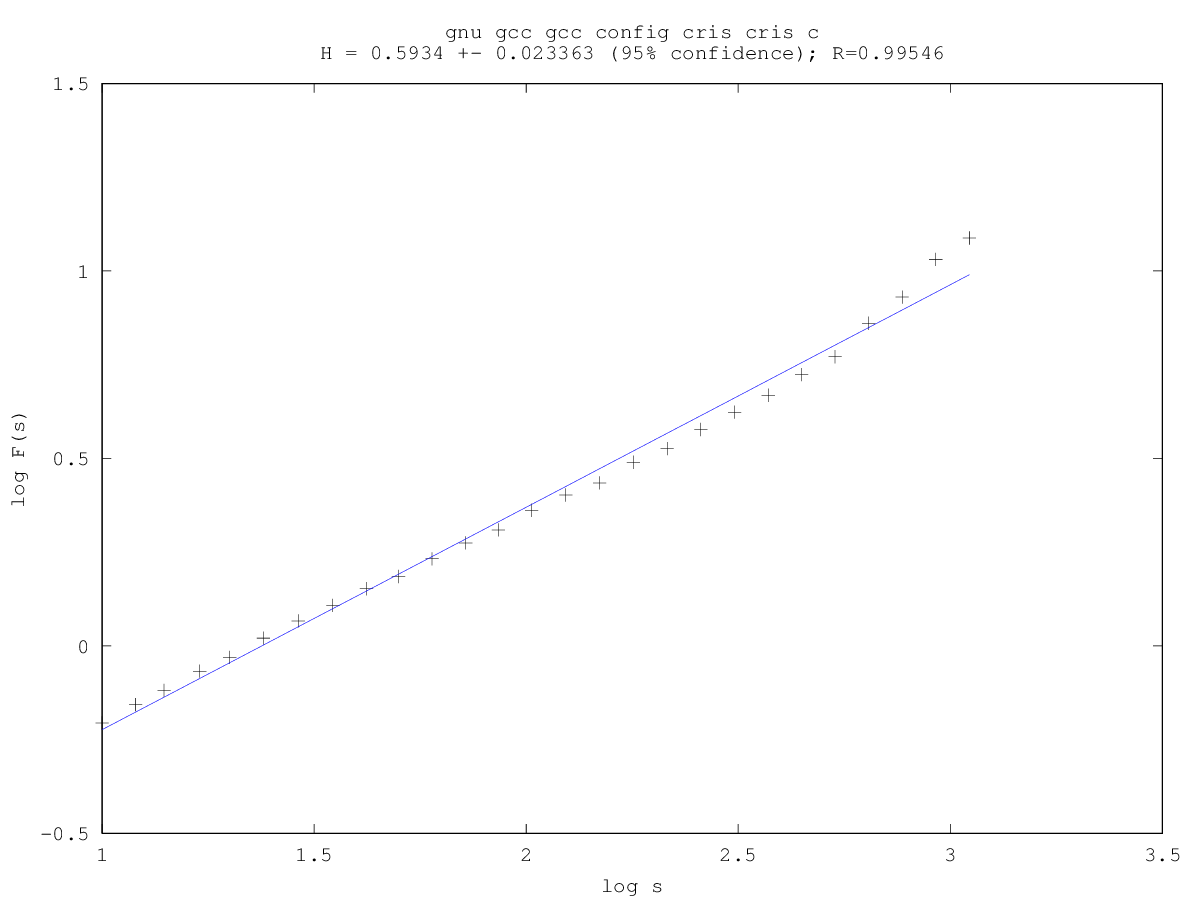
\includegraphics[width=0.8\linewidth]{{fractals/data/gnu_gcc_gcc_config_cris_cris_c_tab3_log_log}.png}
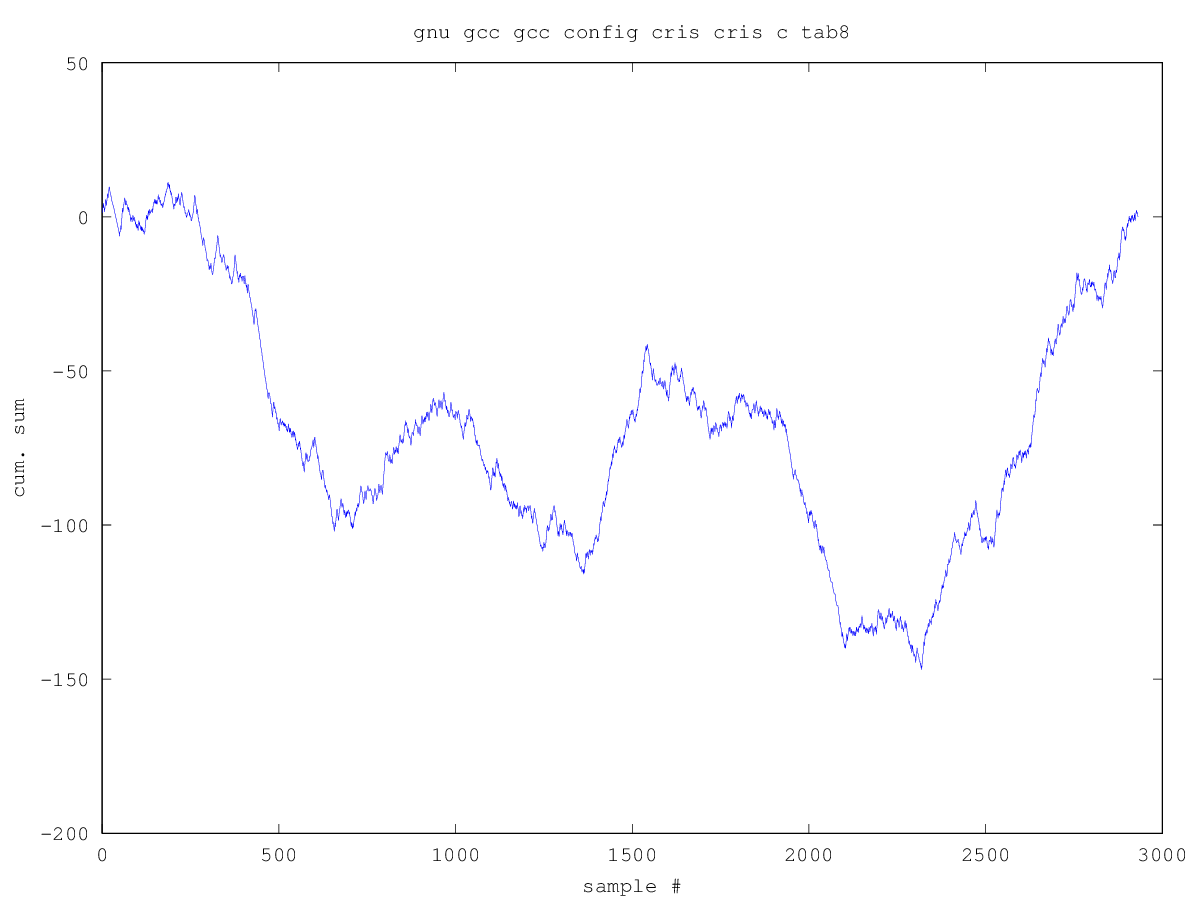
\includegraphics[width=0.8\linewidth]{{fractals/data/gnu_gcc_gcc_config_cris_cris_c_tab8_time_series}.png}
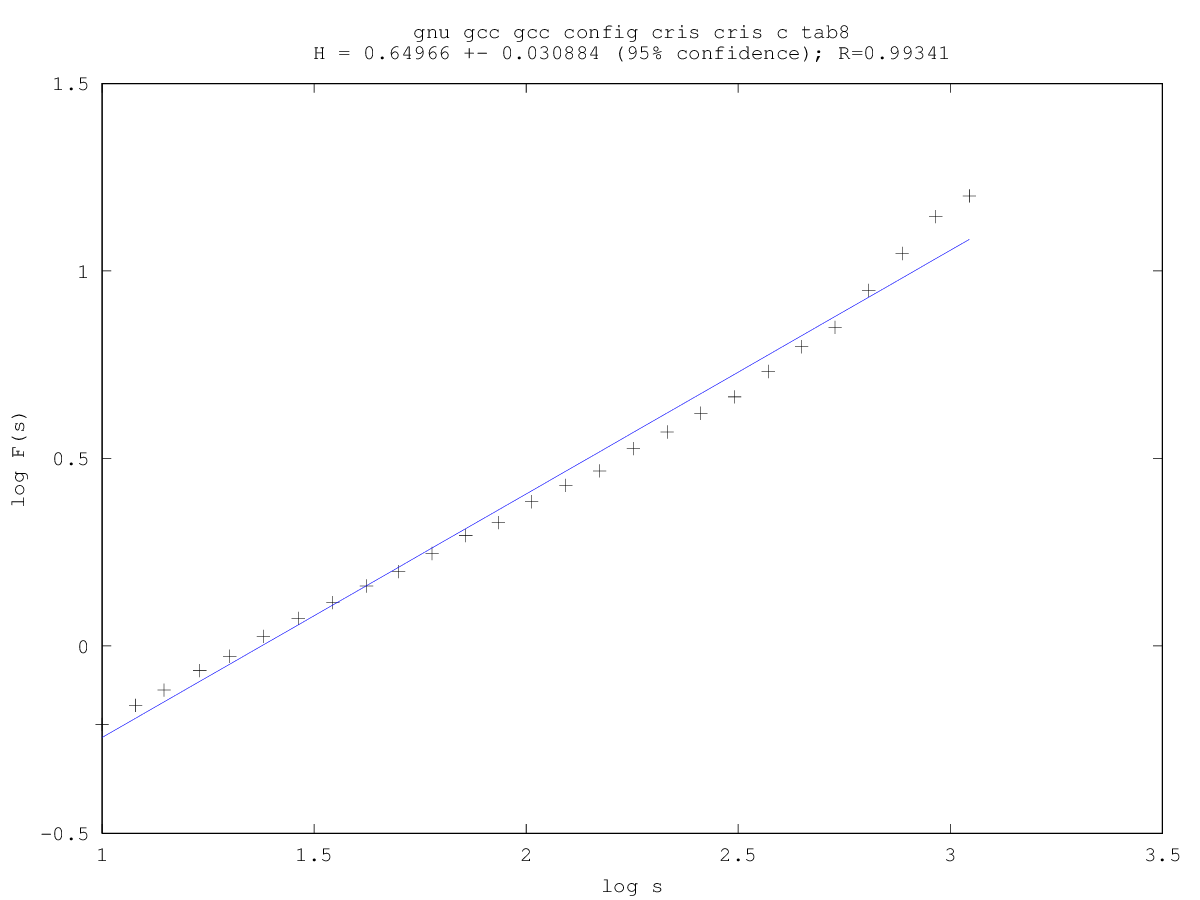
\includegraphics[width=0.8\linewidth]{{fractals/data/gnu_gcc_gcc_config_cris_cris_c_tab8_log_log}.png}
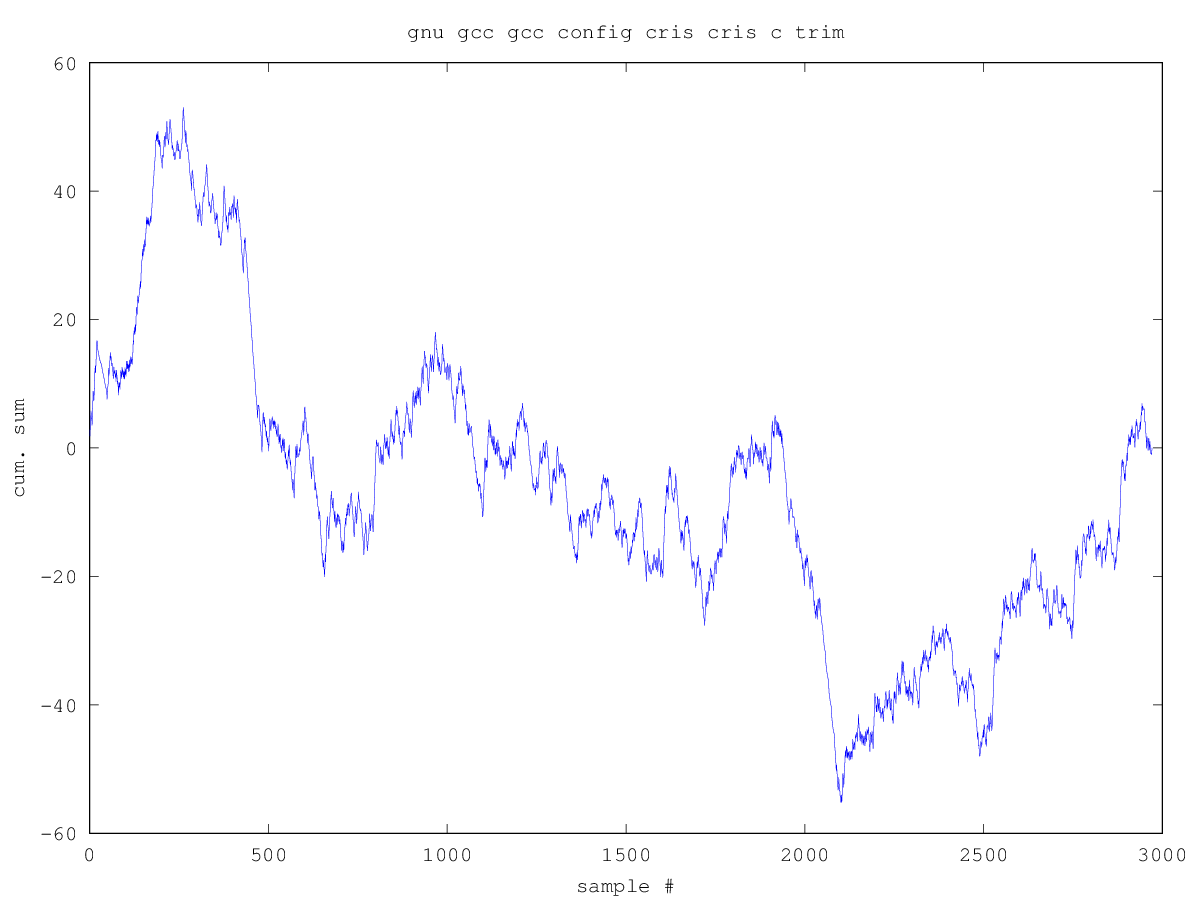
\includegraphics[width=0.8\linewidth]{{fractals/data/gnu_gcc_gcc_config_cris_cris_c_trim_time_series}.png}
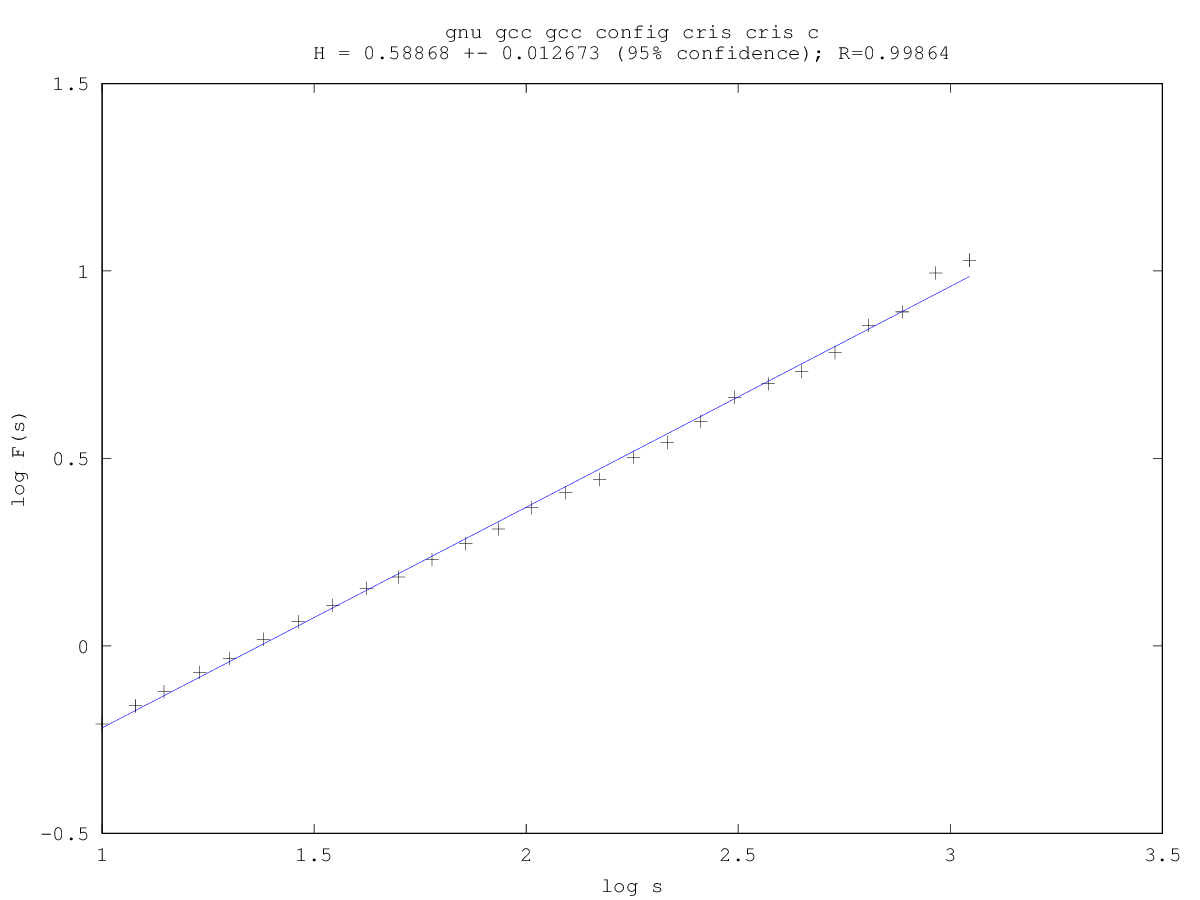
\includegraphics[width=0.8\linewidth]{{fractals/data/gnu_gcc_gcc_config_cris_cris_c_trim_log_log}.png}
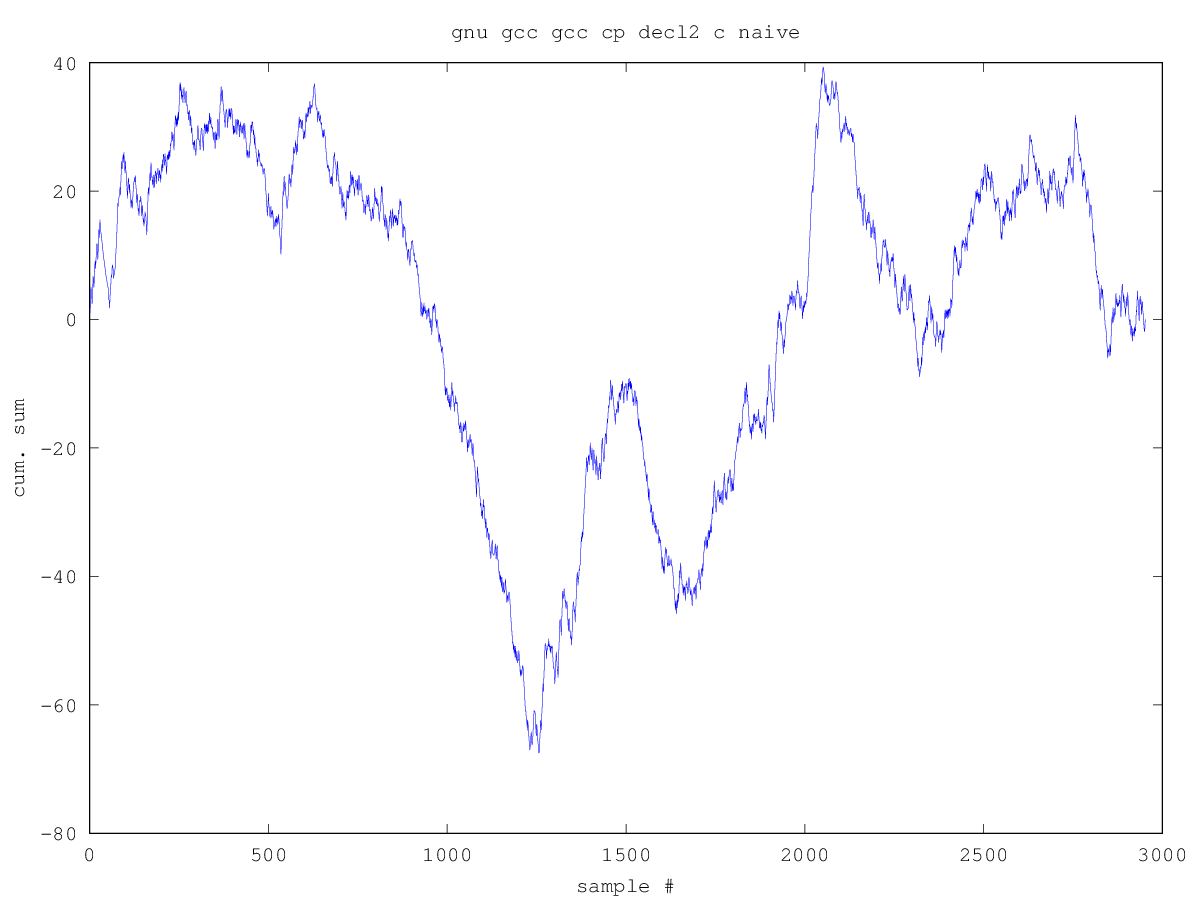
\includegraphics[width=0.8\linewidth]{{fractals/data/gnu_gcc_gcc_cp_decl2_c_naive_time_series}.png}
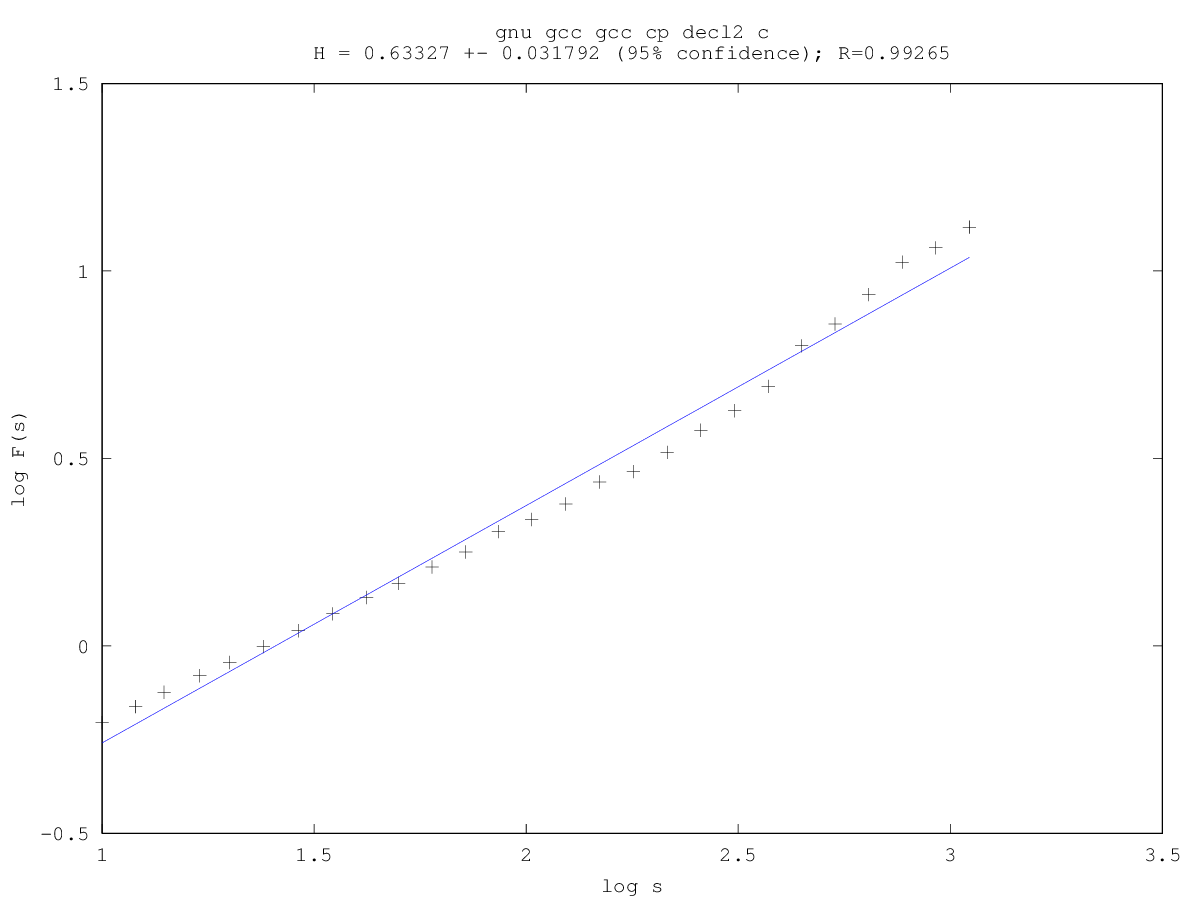
\includegraphics[width=0.8\linewidth]{{fractals/data/gnu_gcc_gcc_cp_decl2_c_naive_log_log}.png}
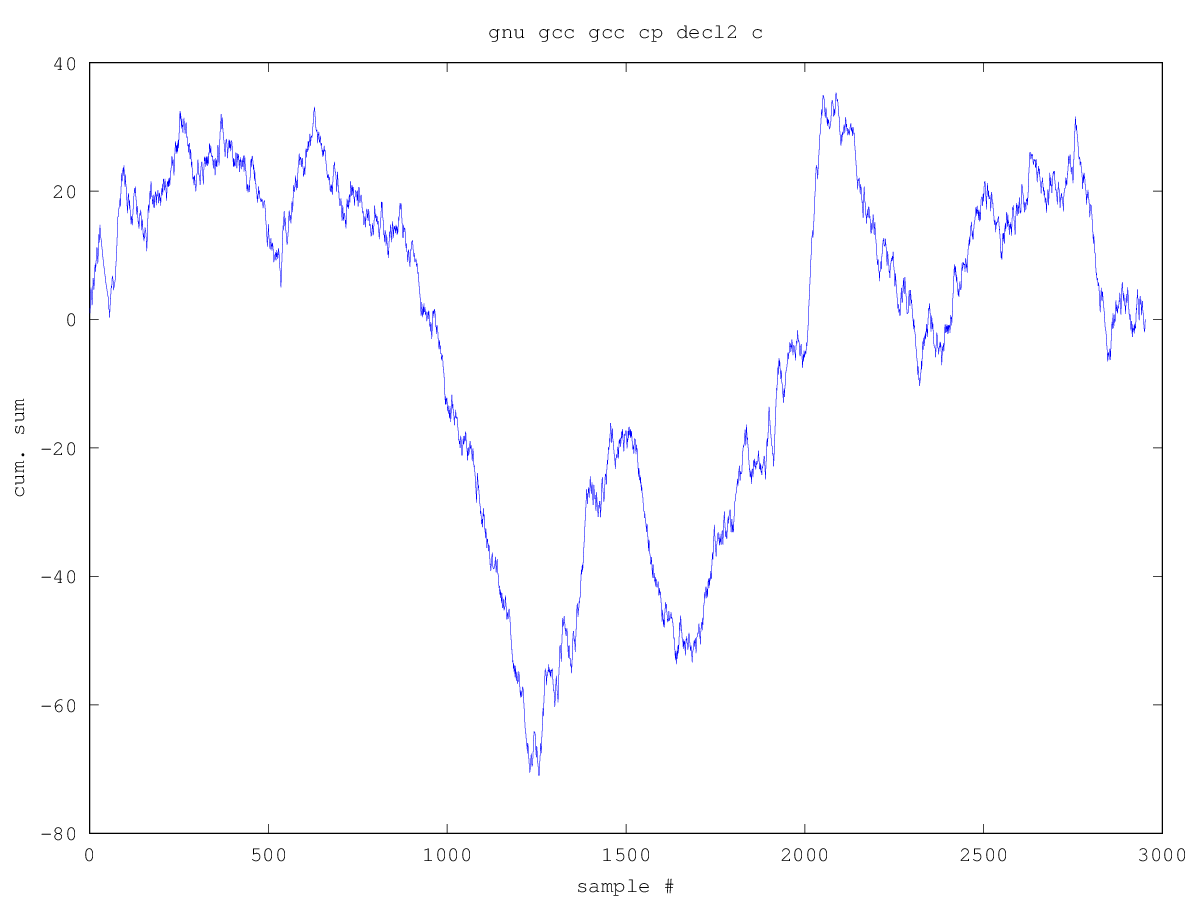
\includegraphics[width=0.8\linewidth]{{fractals/data/gnu_gcc_gcc_cp_decl2_c_tab3_time_series}.png}
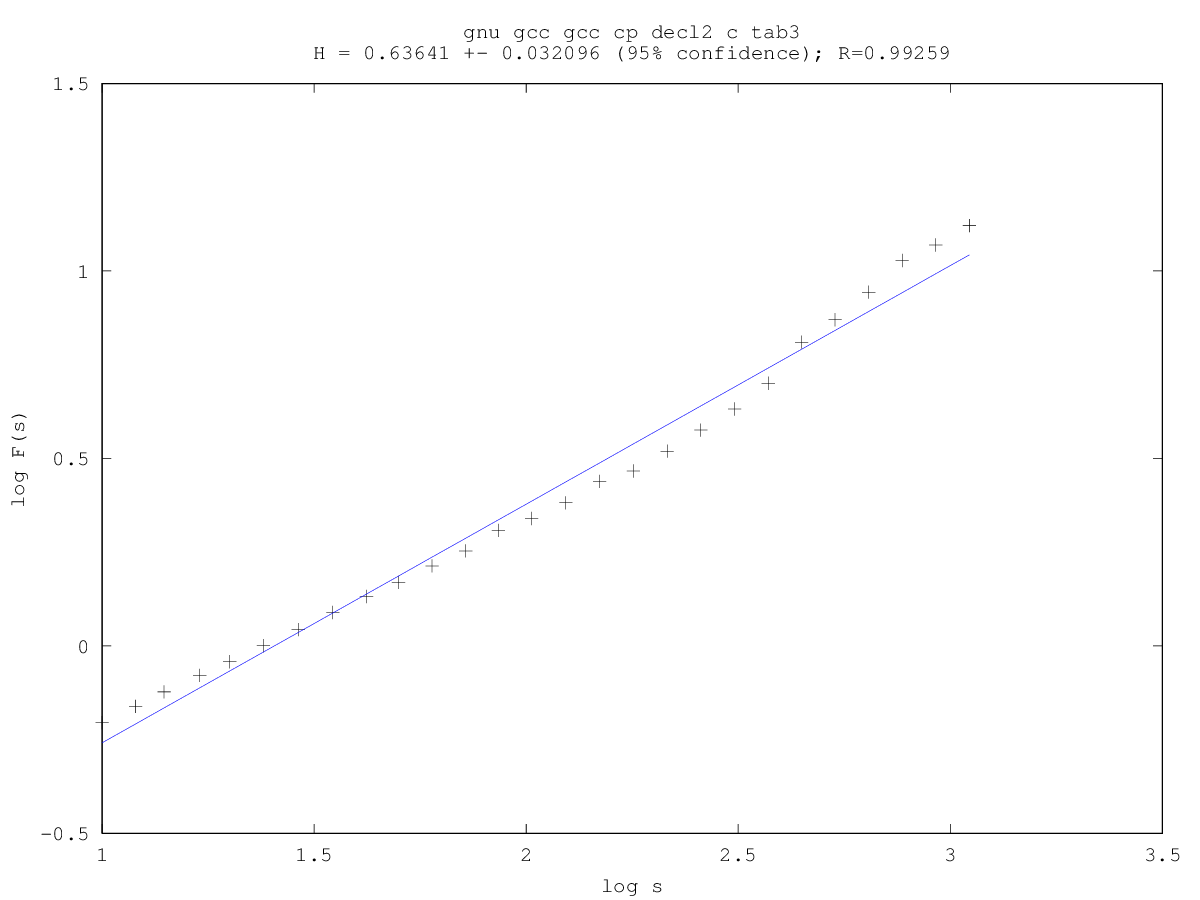
\includegraphics[width=0.8\linewidth]{{fractals/data/gnu_gcc_gcc_cp_decl2_c_tab3_log_log}.png}
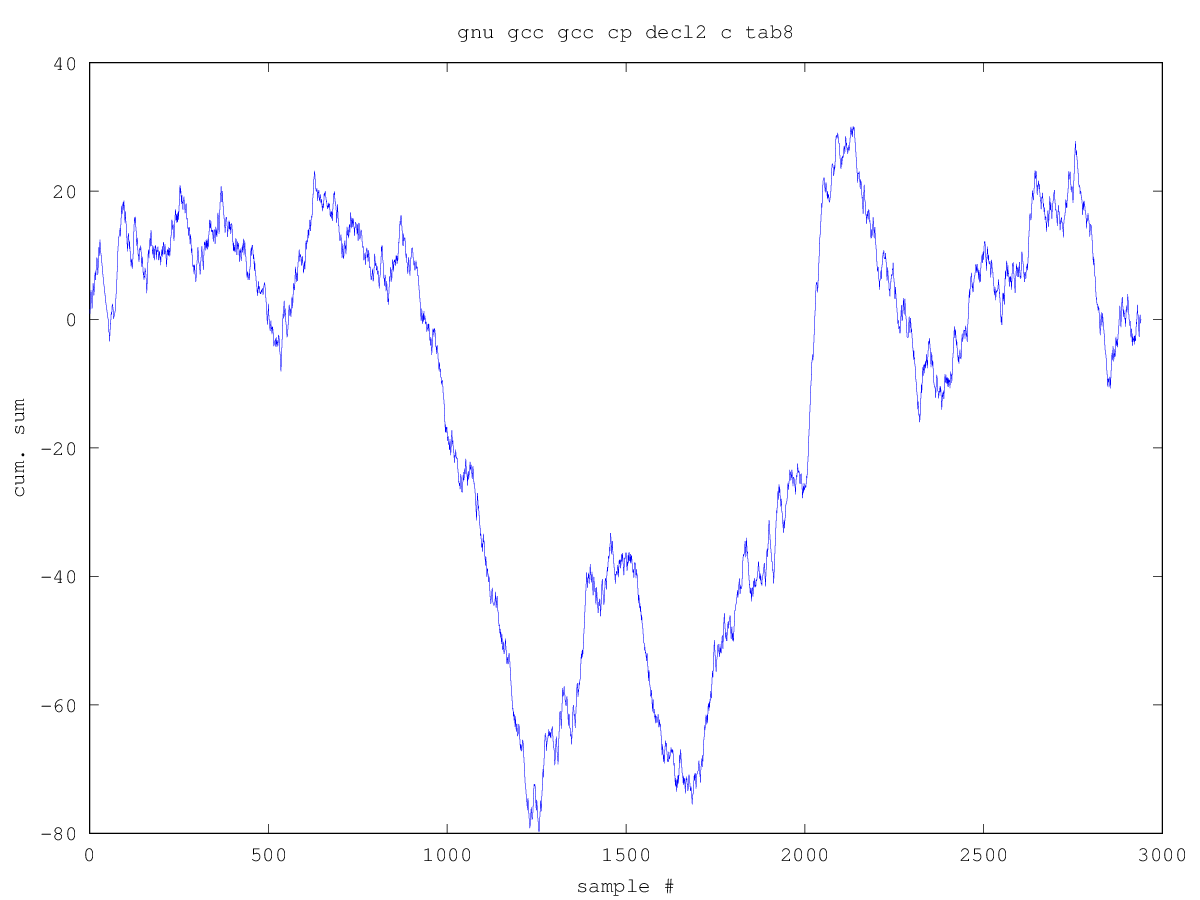
\includegraphics[width=0.8\linewidth]{{fractals/data/gnu_gcc_gcc_cp_decl2_c_tab8_time_series}.png}
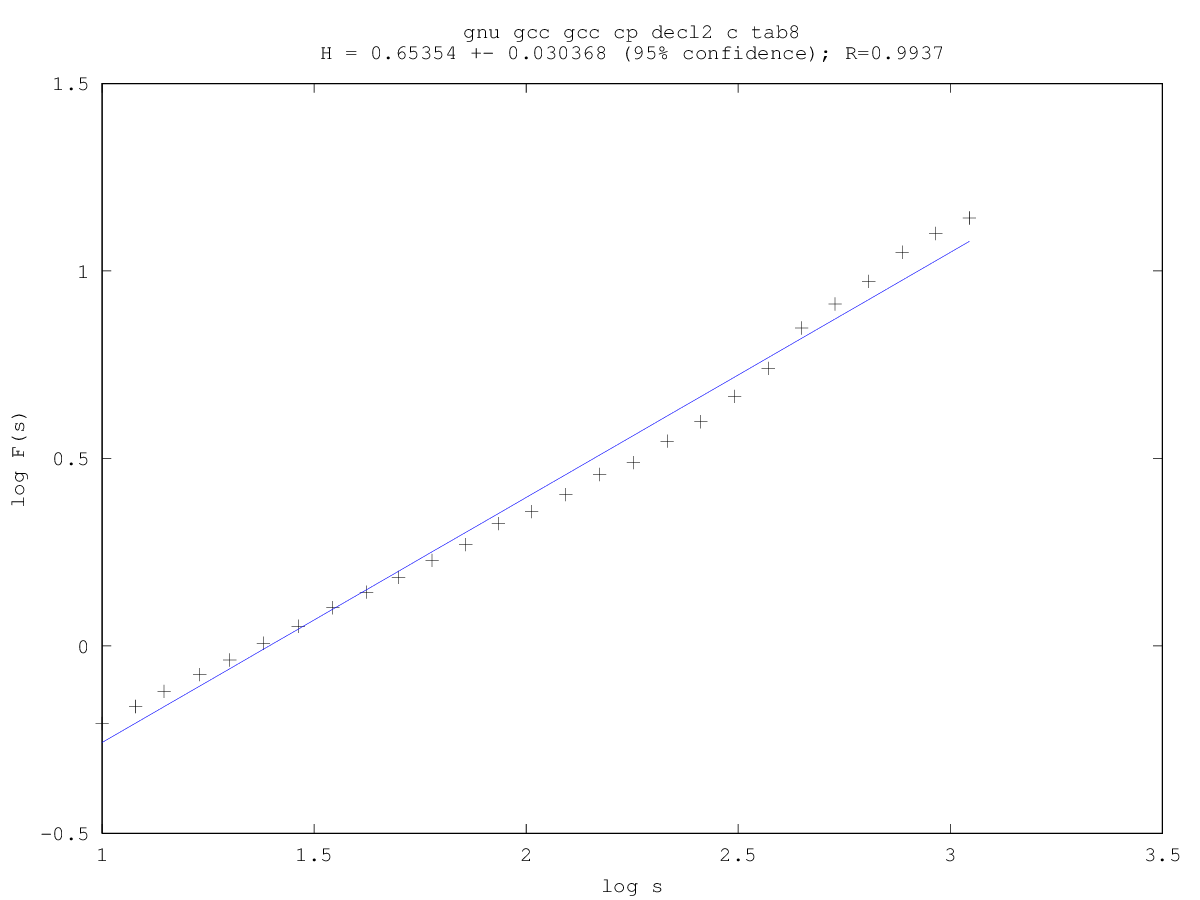
\includegraphics[width=0.8\linewidth]{{fractals/data/gnu_gcc_gcc_cp_decl2_c_tab8_log_log}.png}
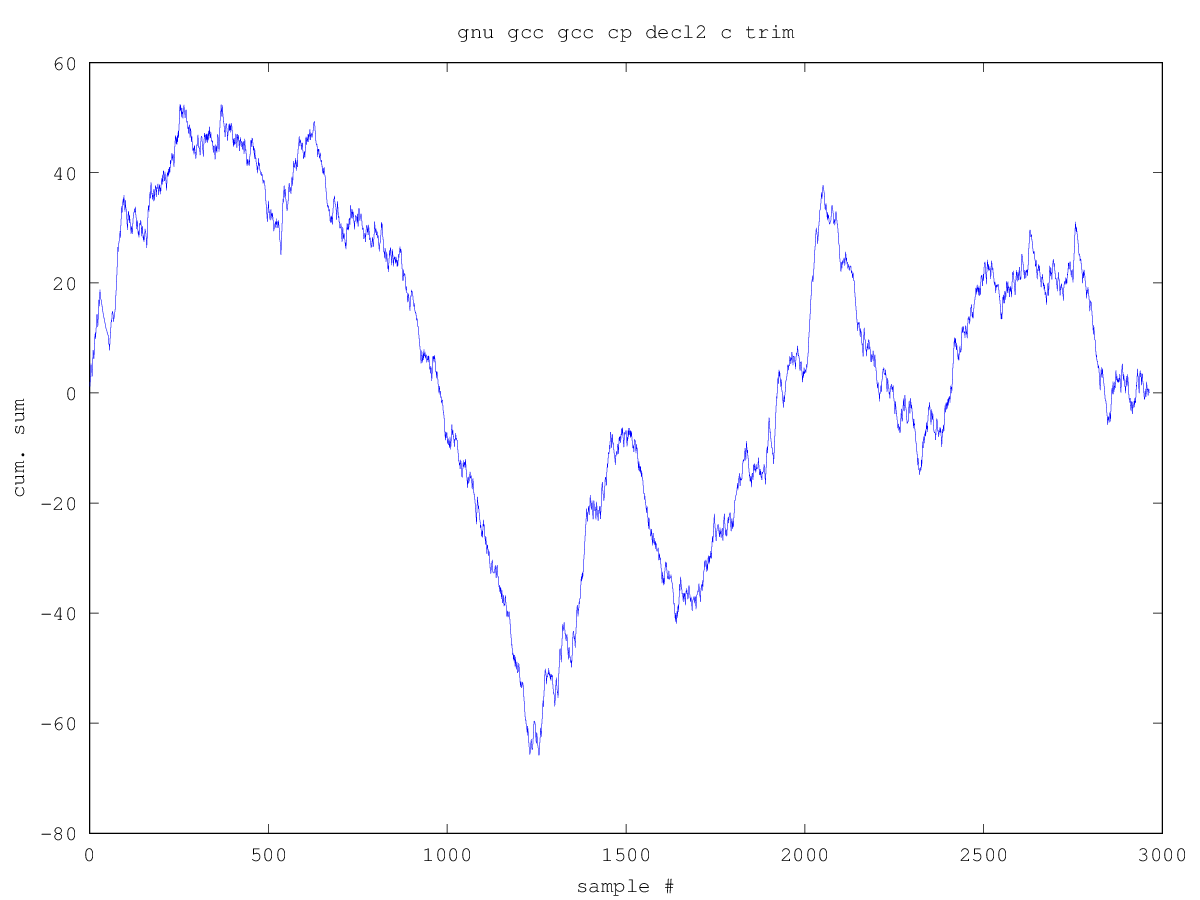
\includegraphics[width=0.8\linewidth]{{fractals/data/gnu_gcc_gcc_cp_decl2_c_trim_time_series}.png}
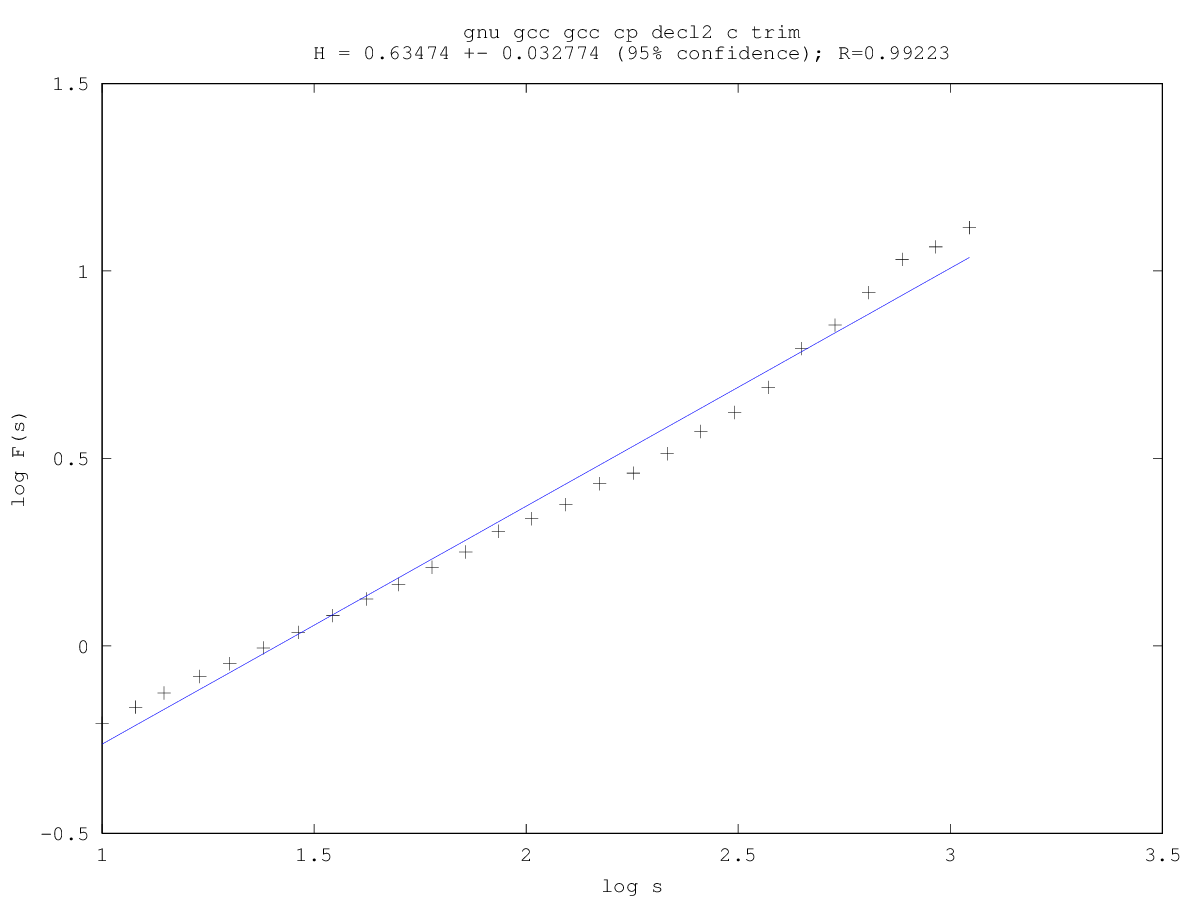
\includegraphics[width=0.8\linewidth]{{fractals/data/gnu_gcc_gcc_cp_decl2_c_trim_log_log}.png}
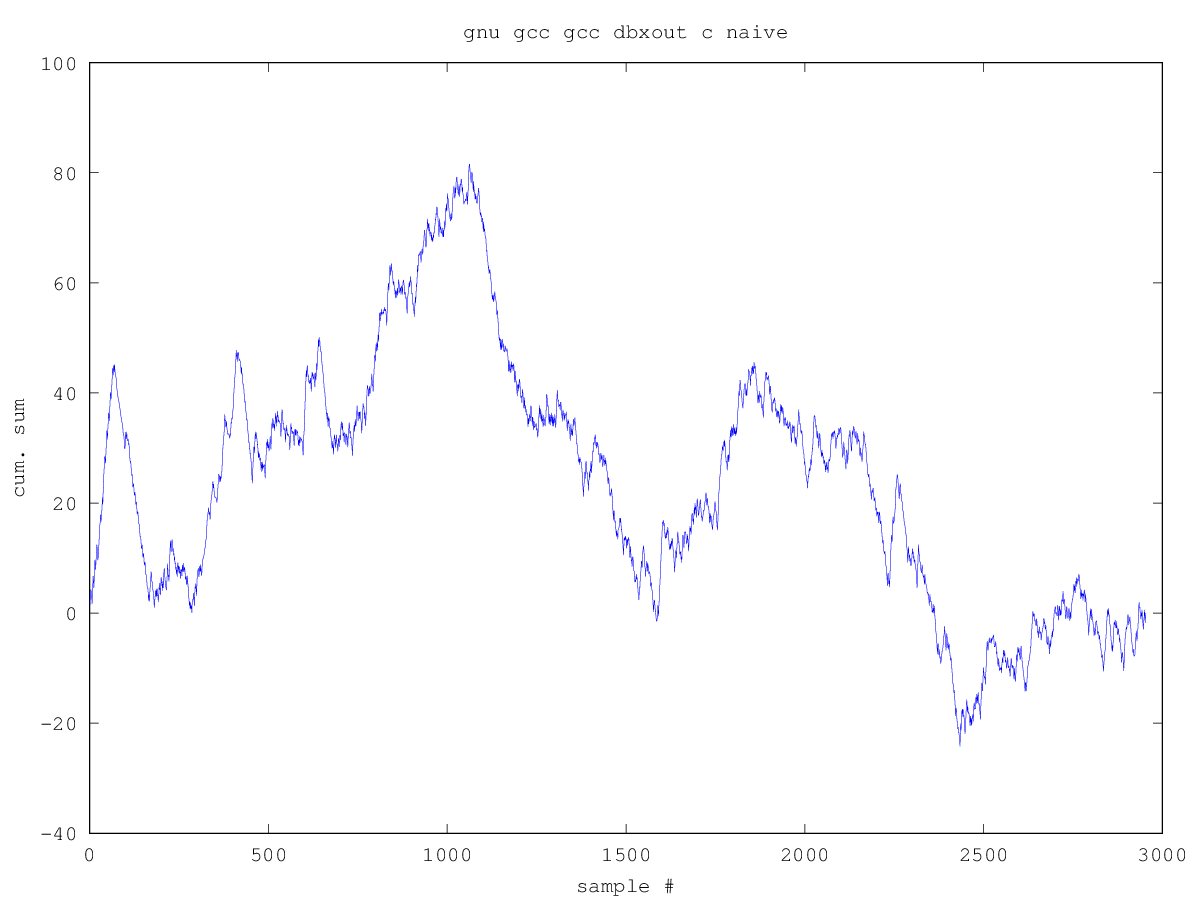
\includegraphics[width=0.8\linewidth]{{fractals/data/gnu_gcc_gcc_dbxout_c_naive_time_series}.png}
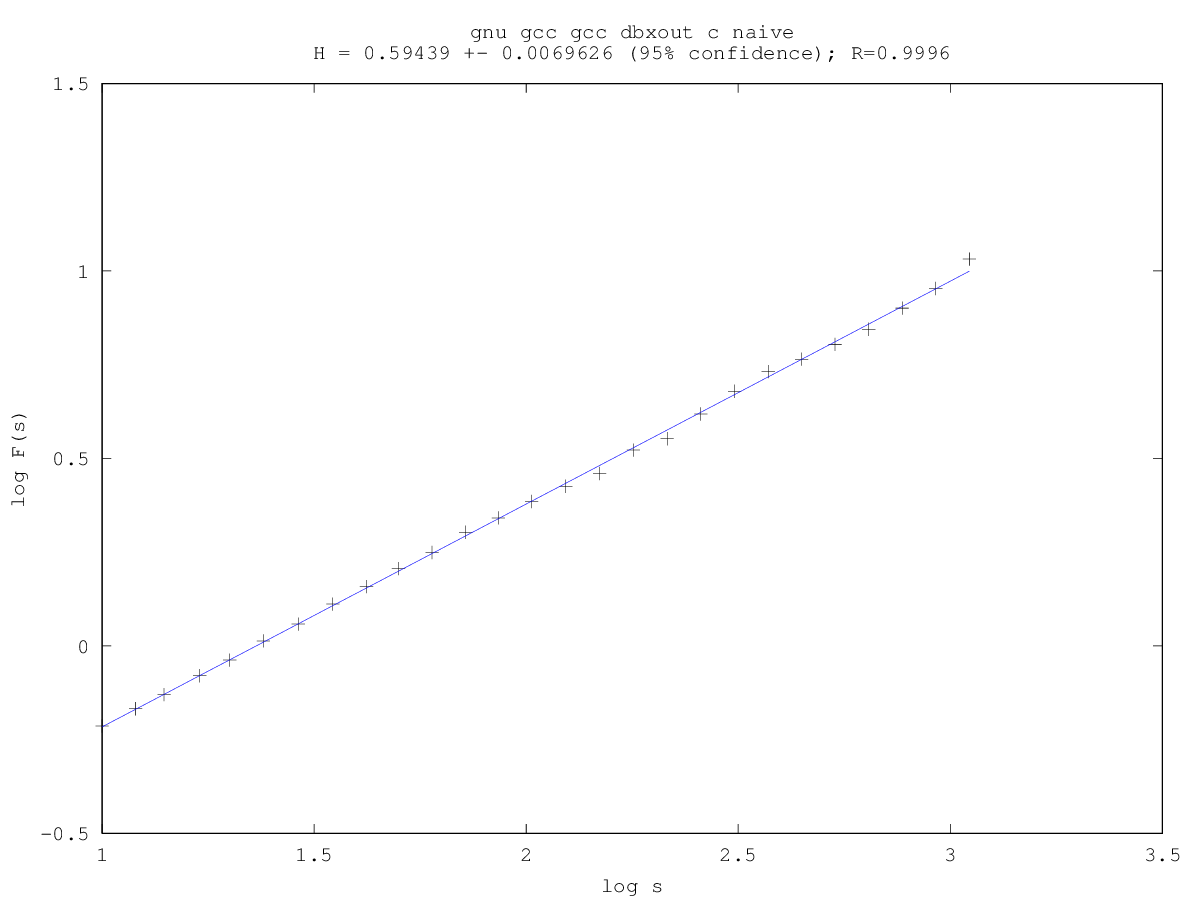
\includegraphics[width=0.8\linewidth]{{fractals/data/gnu_gcc_gcc_dbxout_c_naive_log_log}.png}
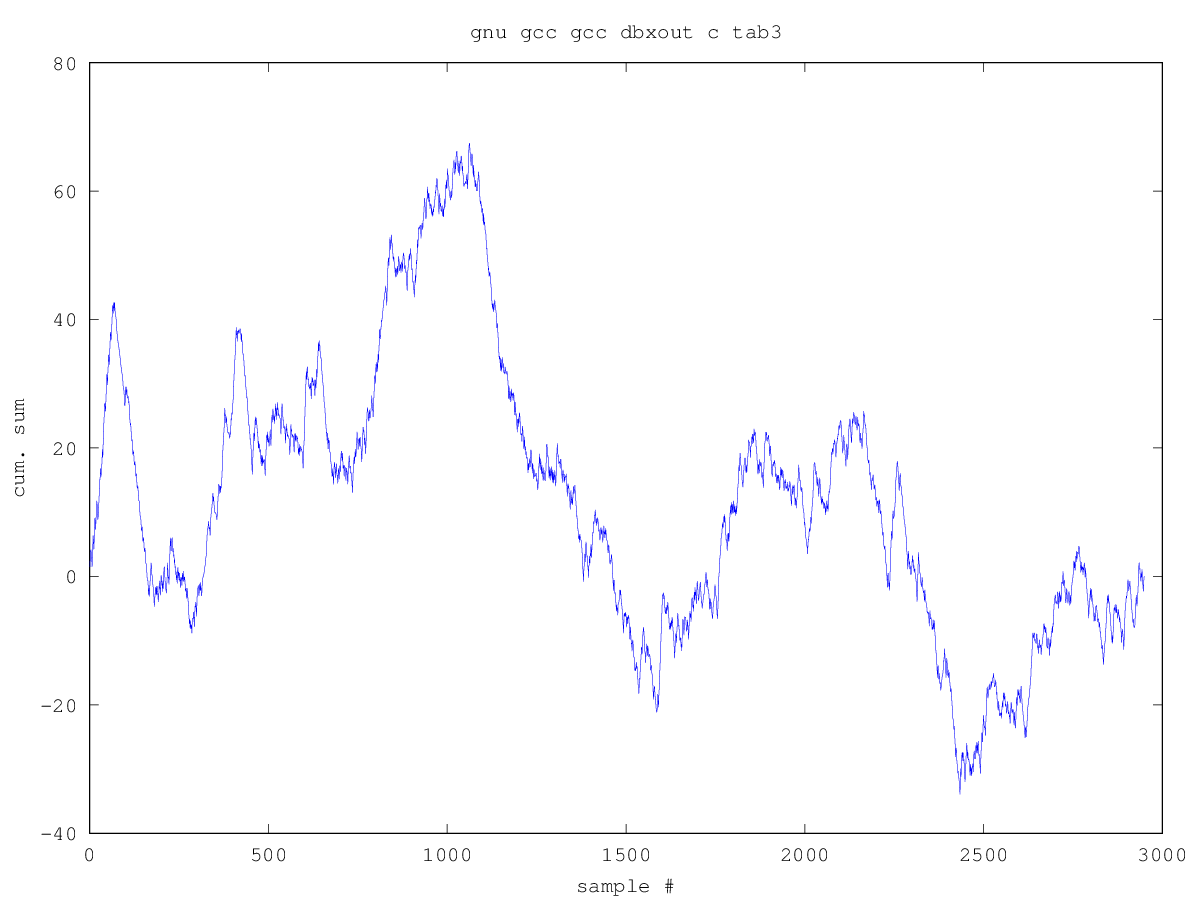
\includegraphics[width=0.8\linewidth]{{fractals/data/gnu_gcc_gcc_dbxout_c_tab3_time_series}.png}
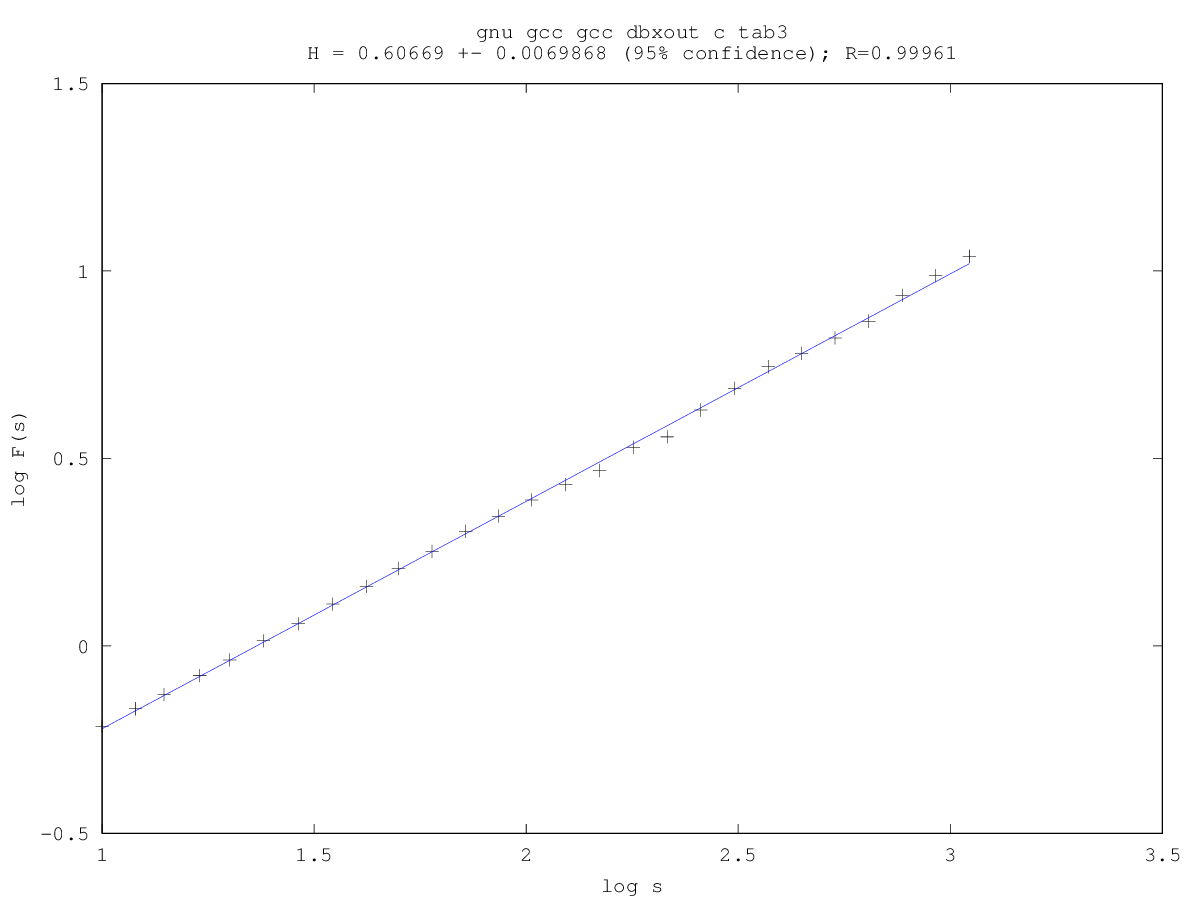
\includegraphics[width=0.8\linewidth]{{fractals/data/gnu_gcc_gcc_dbxout_c_tab3_log_log}.png}
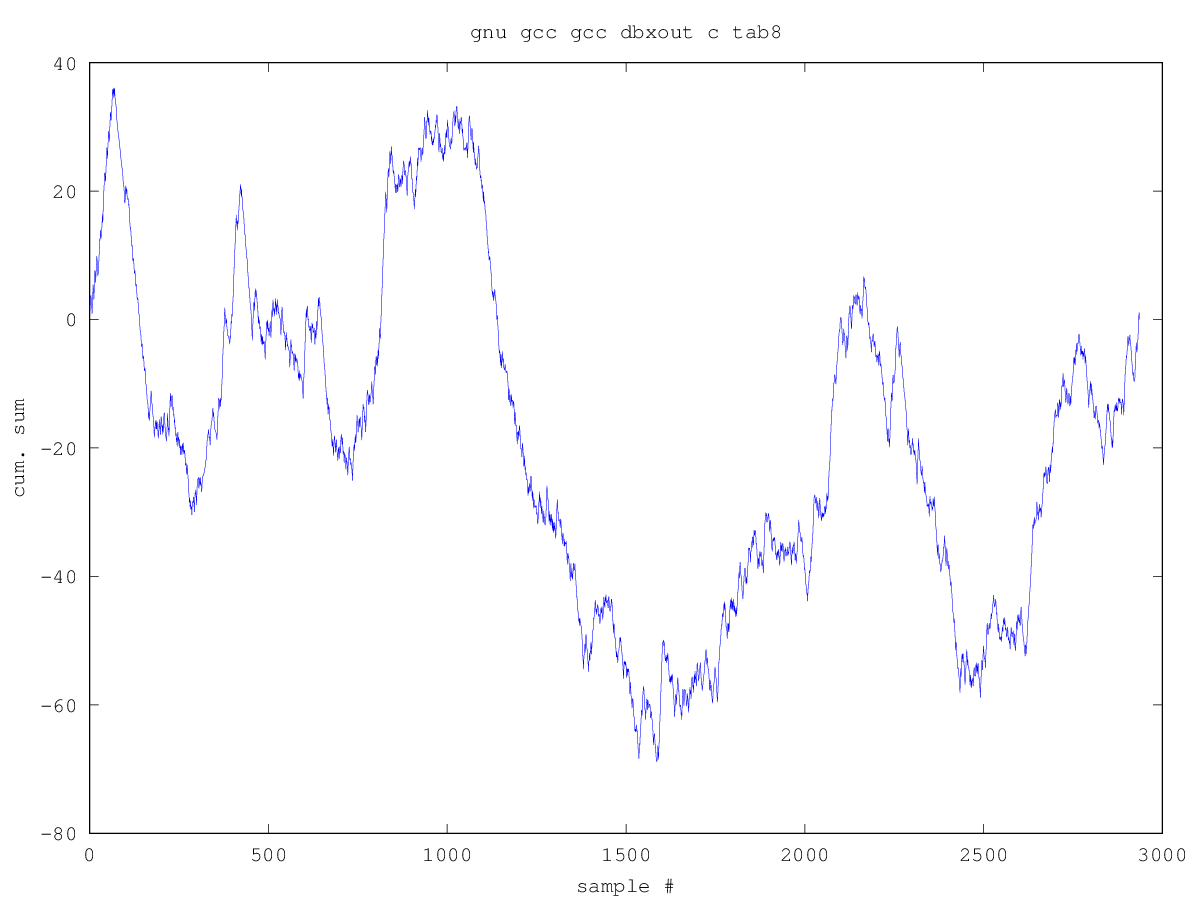
\includegraphics[width=0.8\linewidth]{{fractals/data/gnu_gcc_gcc_dbxout_c_tab8_time_series}.png}
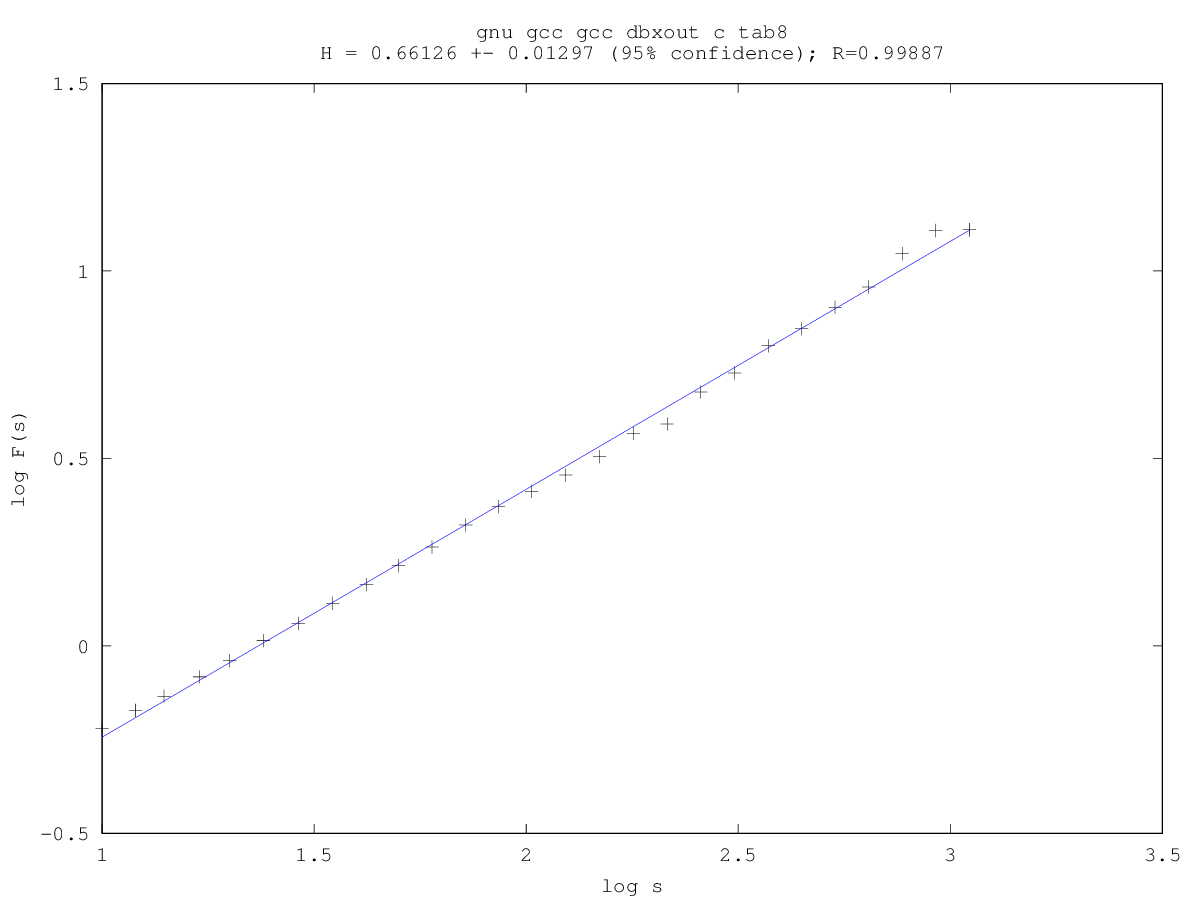
\includegraphics[width=0.8\linewidth]{{fractals/data/gnu_gcc_gcc_dbxout_c_tab8_log_log}.png}
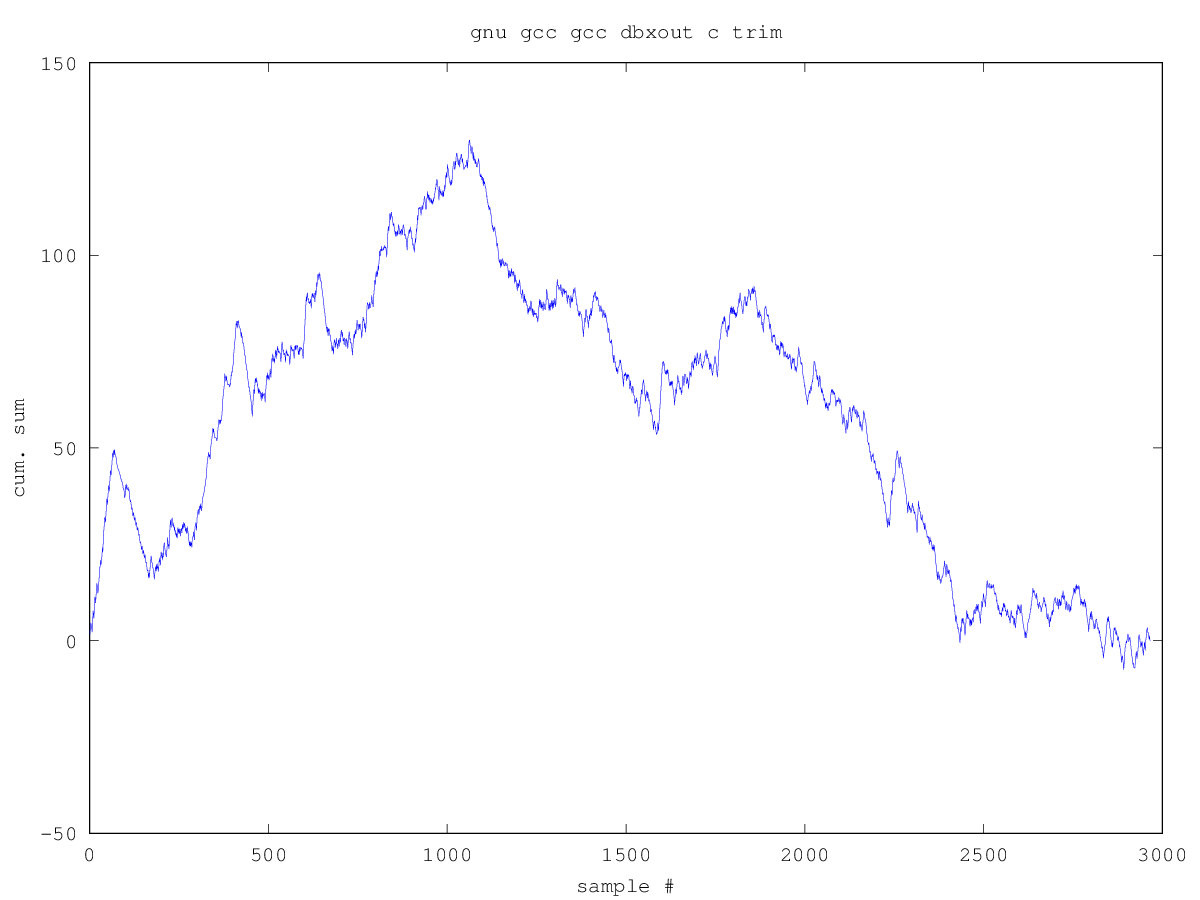
\includegraphics[width=0.8\linewidth]{{fractals/data/gnu_gcc_gcc_dbxout_c_trim_time_series}.png}
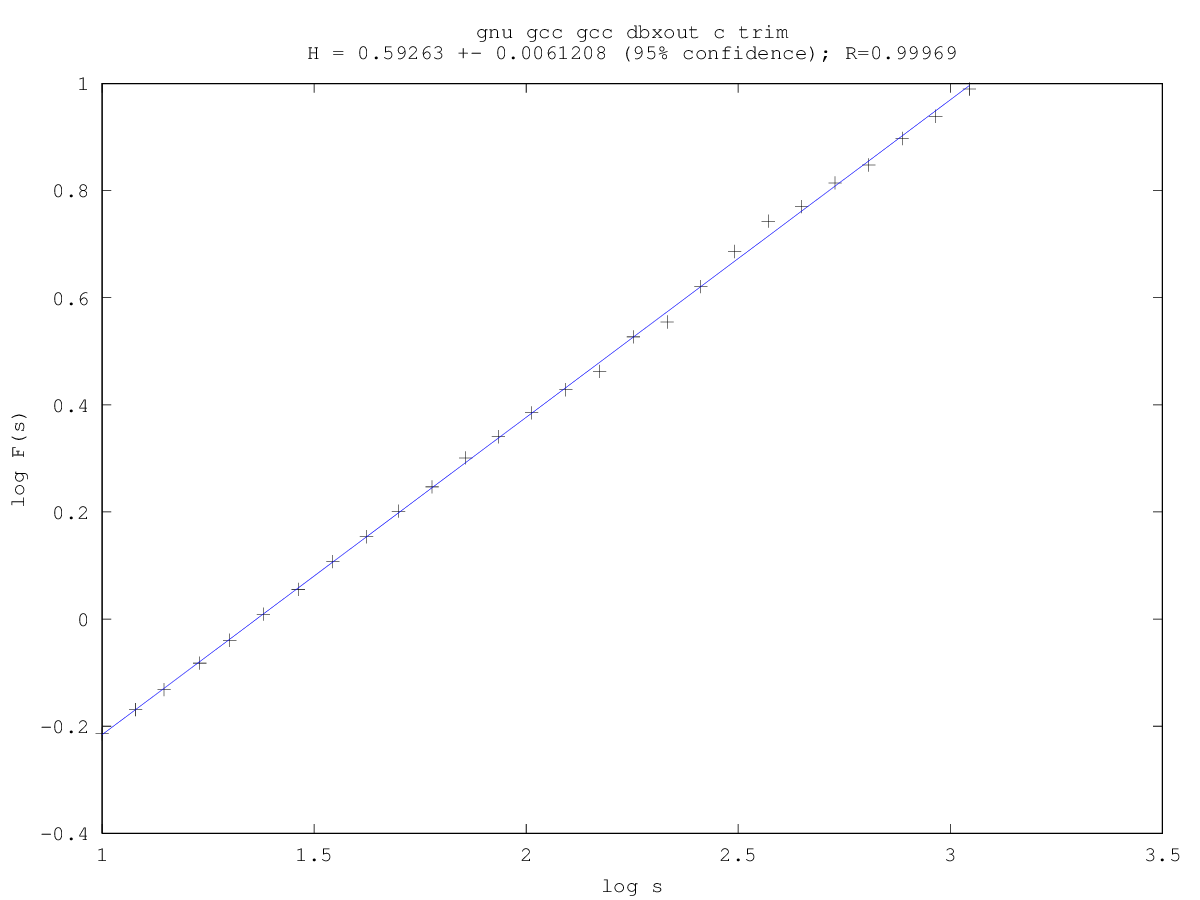
\includegraphics[width=0.8\linewidth]{{fractals/data/gnu_gcc_gcc_dbxout_c_trim_log_log}.png}
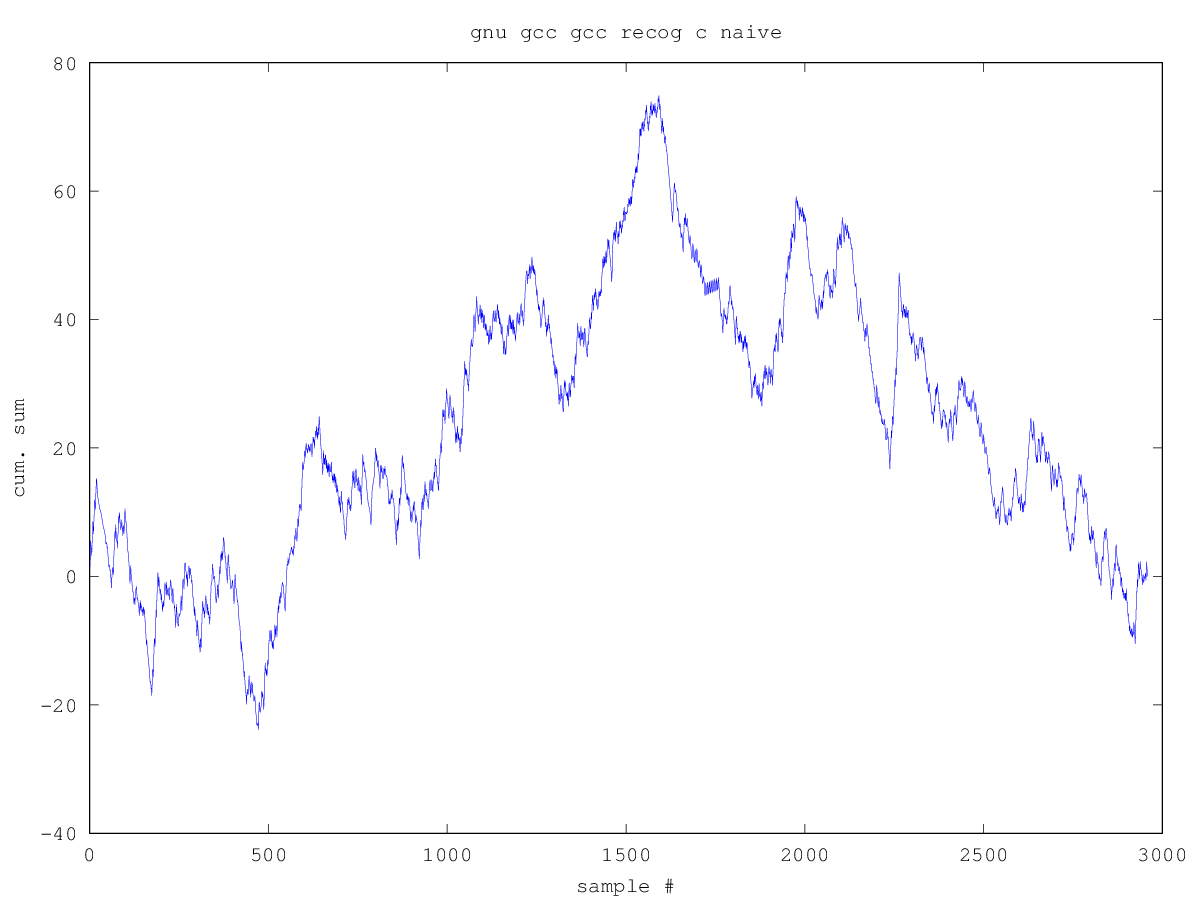
\includegraphics[width=0.8\linewidth]{{fractals/data/gnu_gcc_gcc_recog_c_naive_time_series}.png}
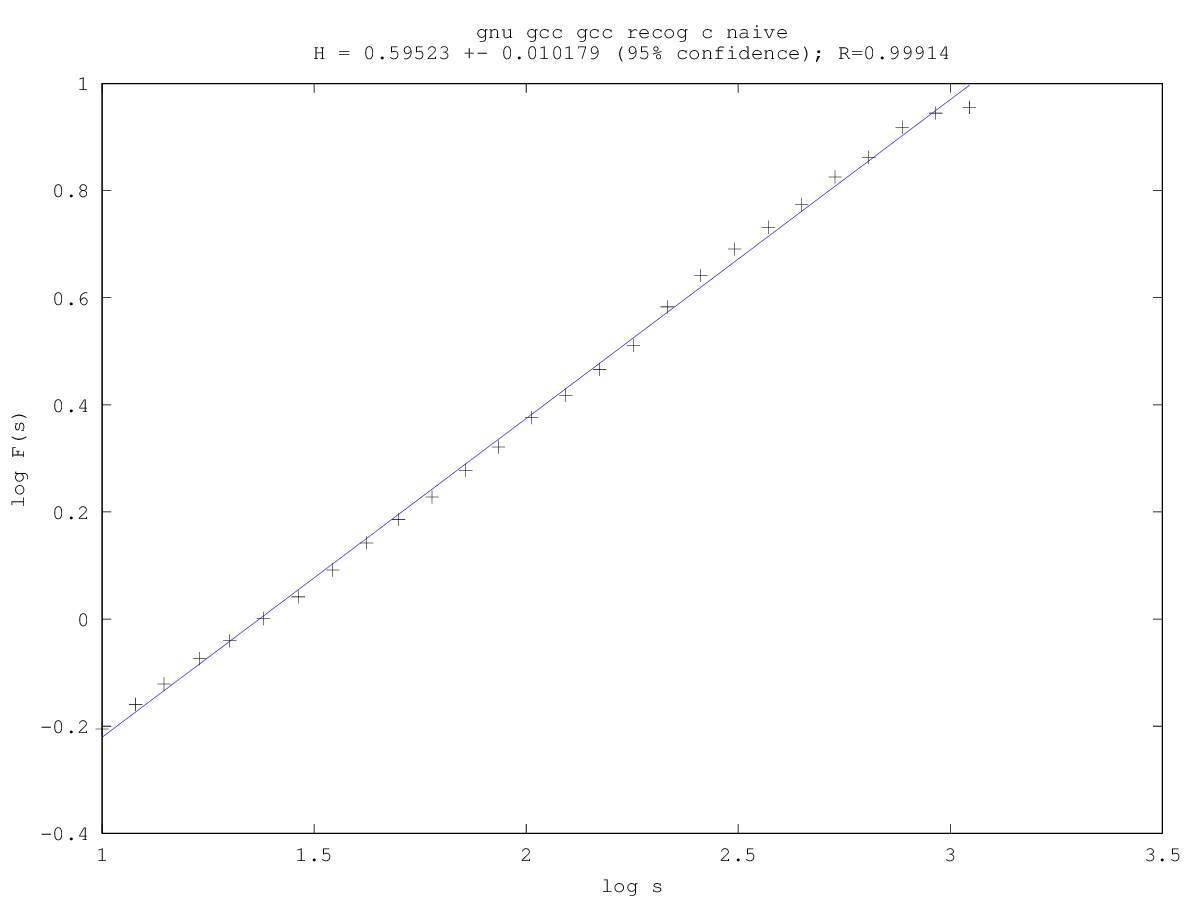
\includegraphics[width=0.8\linewidth]{{fractals/data/gnu_gcc_gcc_recog_c_naive_log_log}.png}
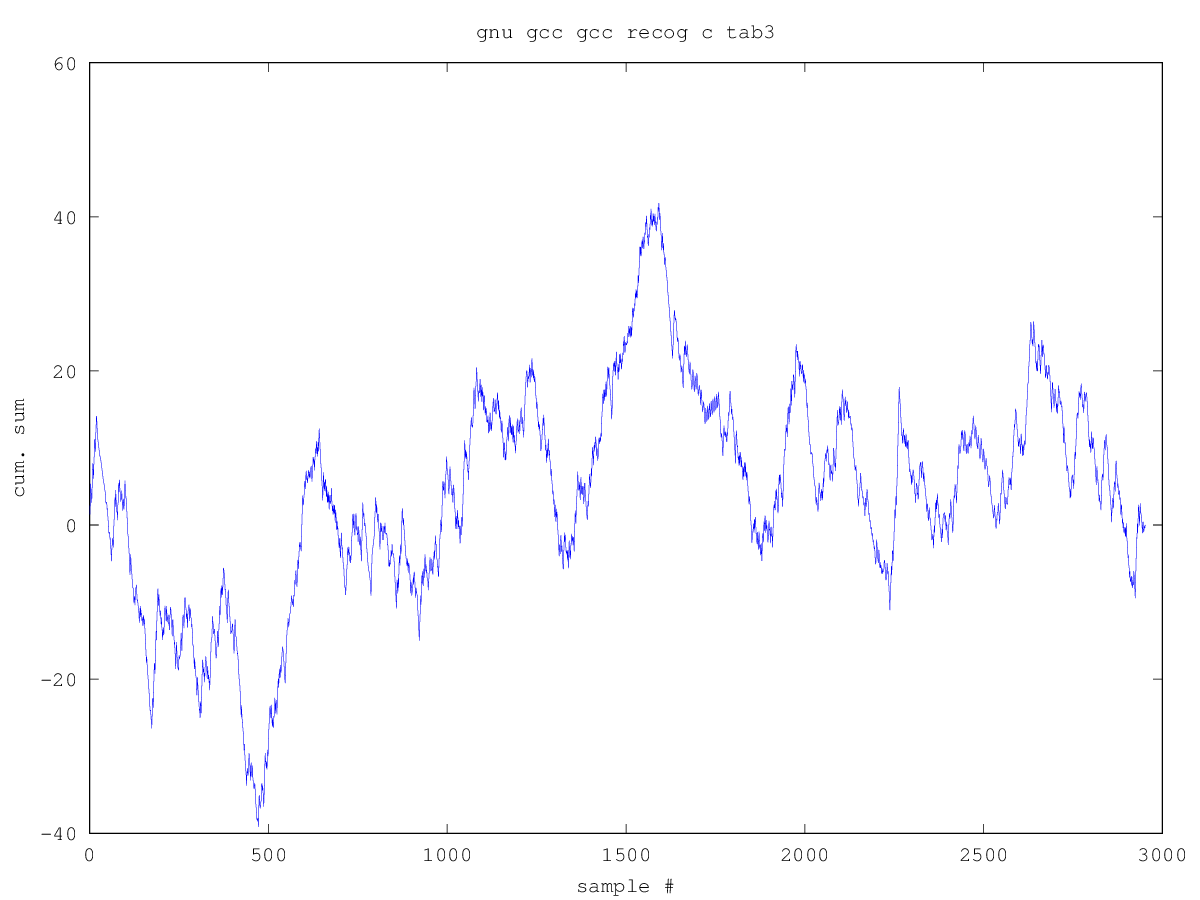
\includegraphics[width=0.8\linewidth]{{fractals/data/gnu_gcc_gcc_recog_c_tab3_time_series}.png}
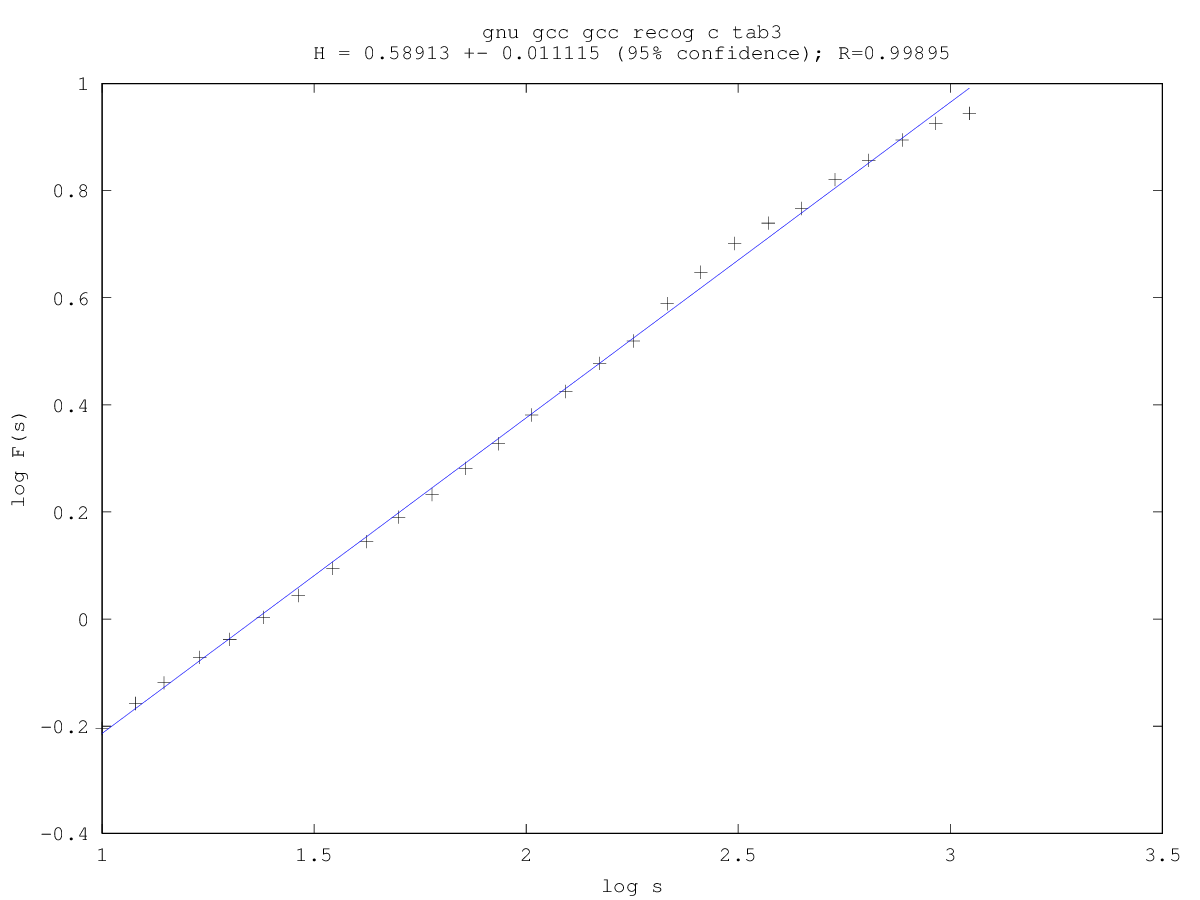
\includegraphics[width=0.8\linewidth]{{fractals/data/gnu_gcc_gcc_recog_c_tab3_log_log}.png}
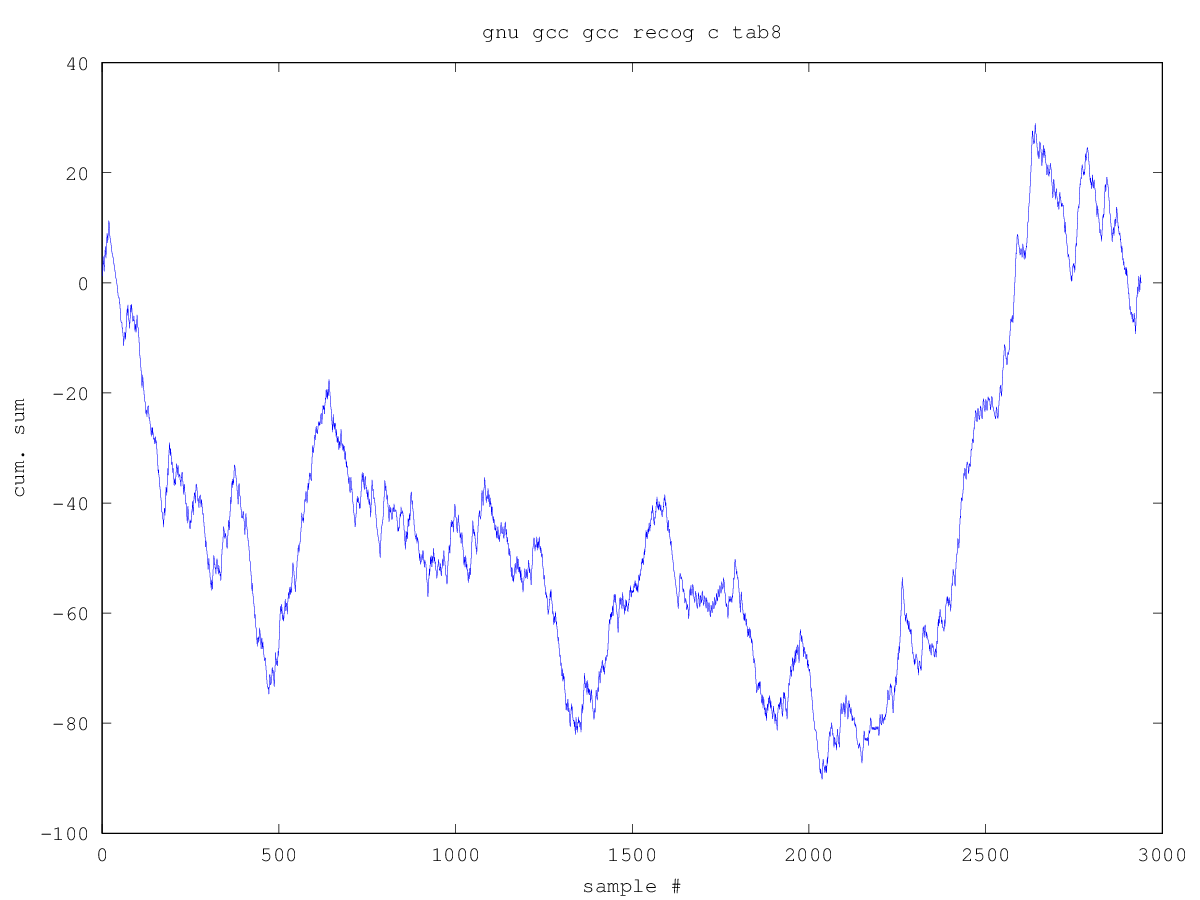
\includegraphics[width=0.8\linewidth]{{fractals/data/gnu_gcc_gcc_recog_c_tab8_time_series}.png}
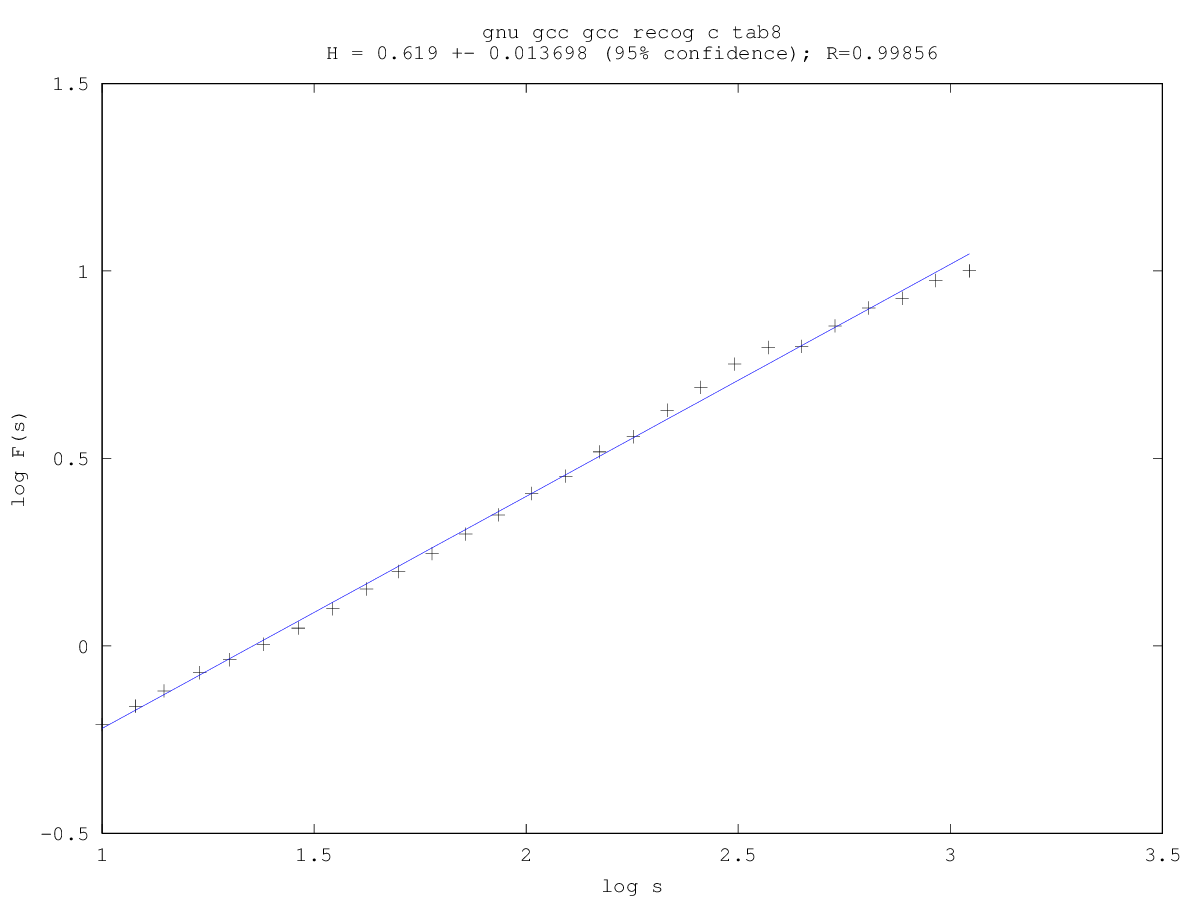
\includegraphics[width=0.8\linewidth]{{fractals/data/gnu_gcc_gcc_recog_c_tab8_log_log}.png}
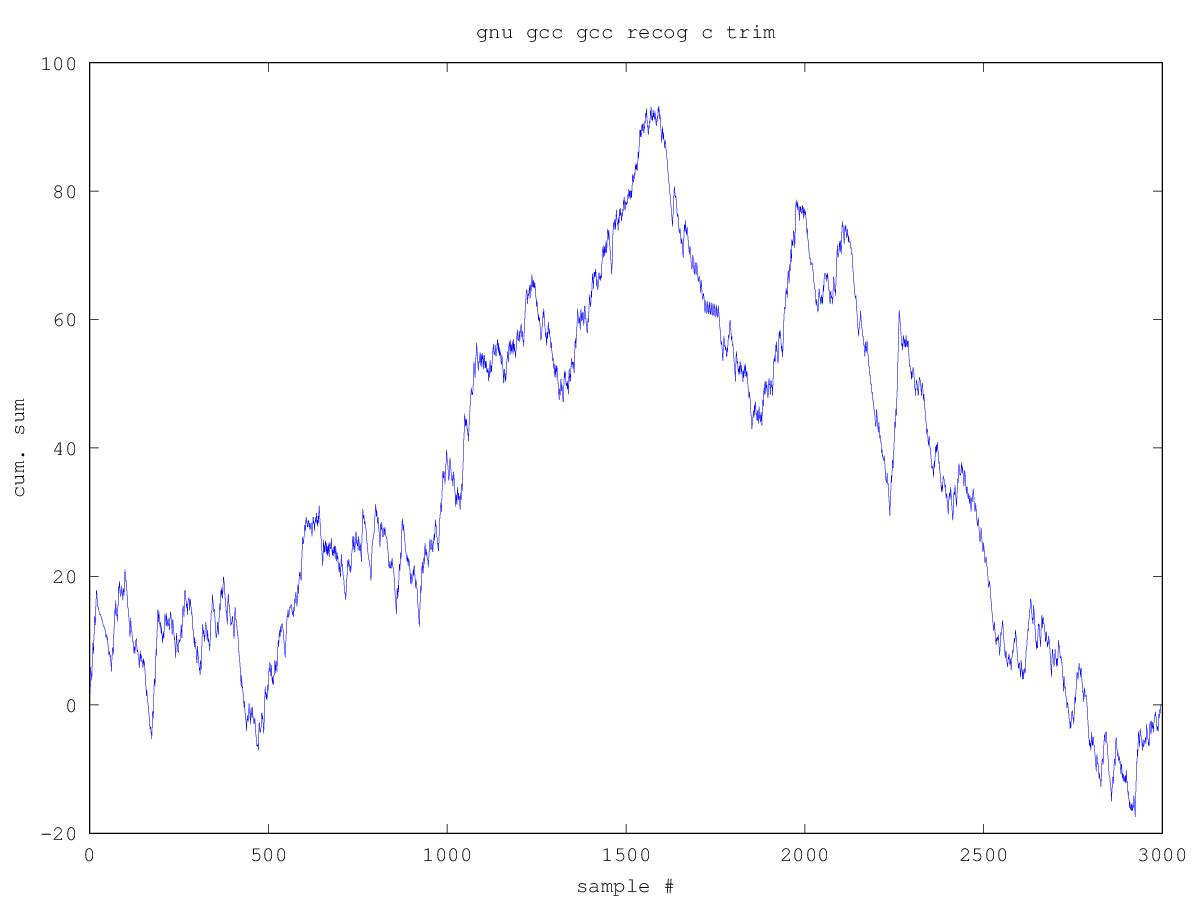
\includegraphics[width=0.8\linewidth]{{fractals/data/gnu_gcc_gcc_recog_c_trim_time_series}.png}
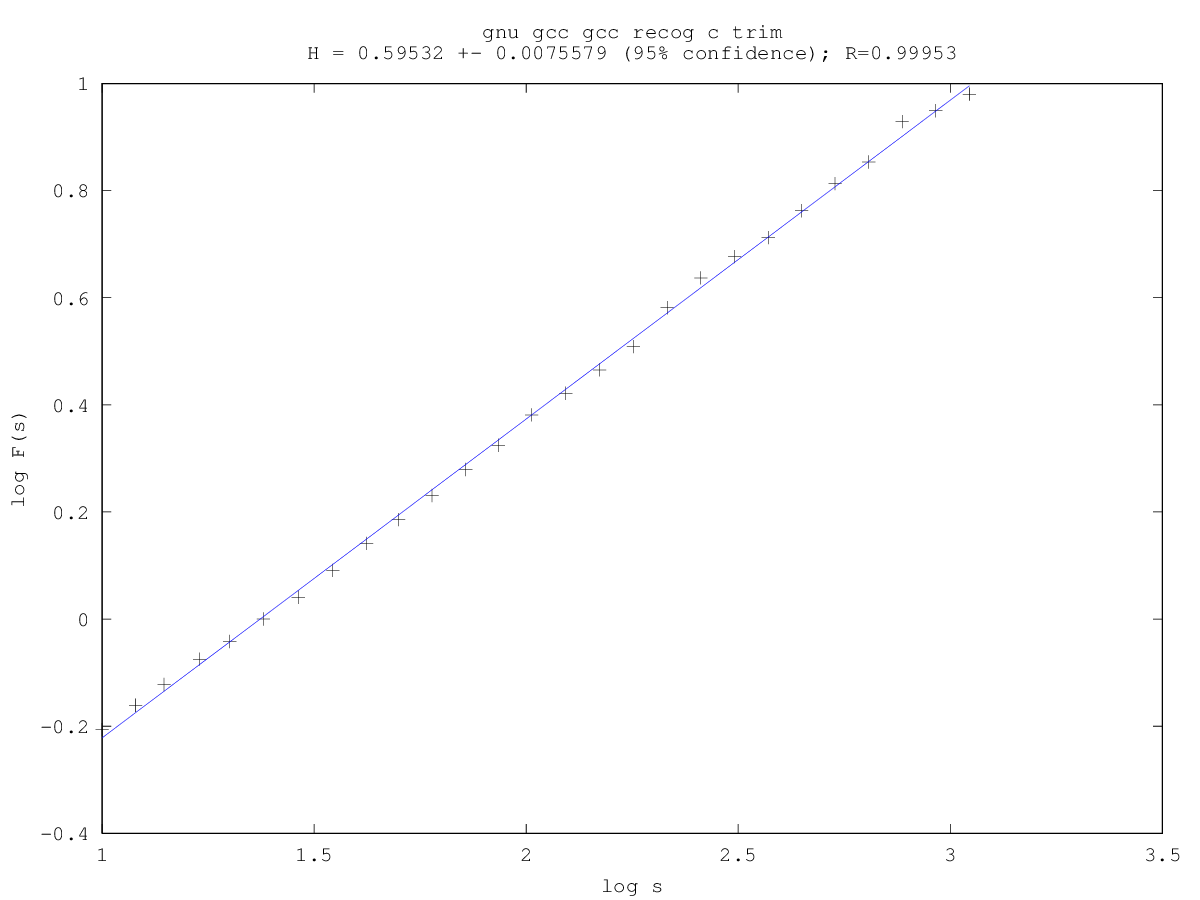
\includegraphics[width=0.8\linewidth]{{fractals/data/gnu_gcc_gcc_recog_c_trim_log_log}.png}
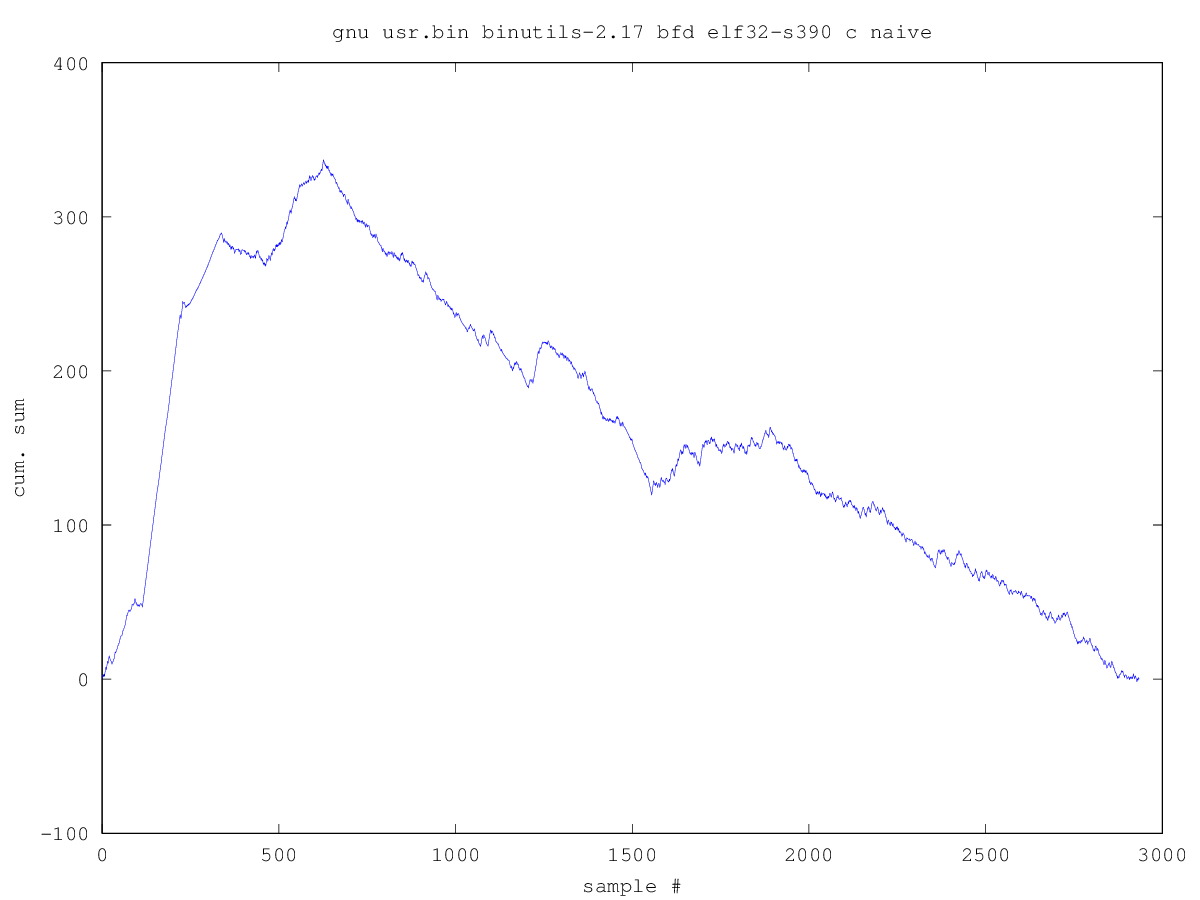
\includegraphics[width=0.8\linewidth]{{fractals/data/gnu_usr.bin_binutils-2.17_bfd_elf32-s390_c_naive_time_series}.png}
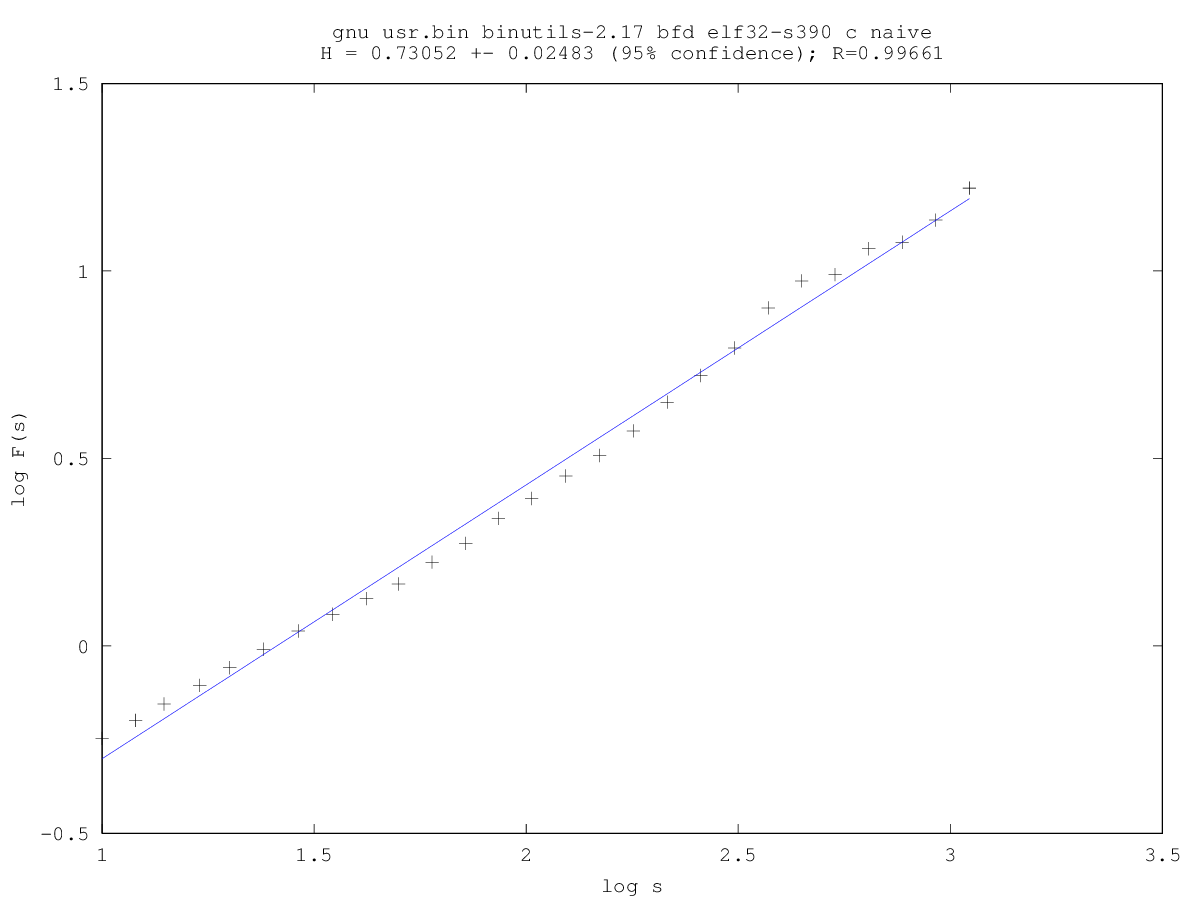
\includegraphics[width=0.8\linewidth]{{fractals/data/gnu_usr.bin_binutils-2.17_bfd_elf32-s390_c_naive_log_log}.png}
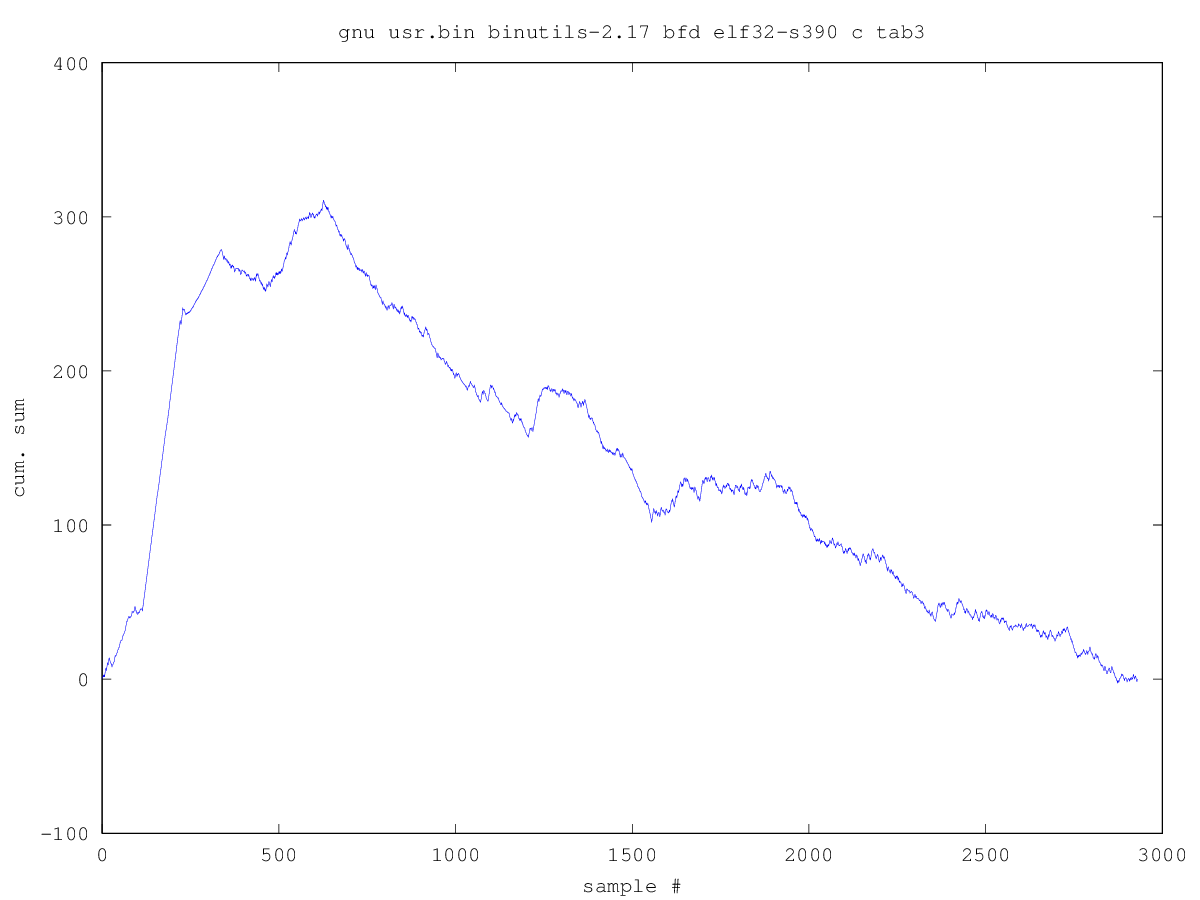
\includegraphics[width=0.8\linewidth]{{fractals/data/gnu_usr.bin_binutils-2.17_bfd_elf32-s390_c_tab3_time_series}.png}
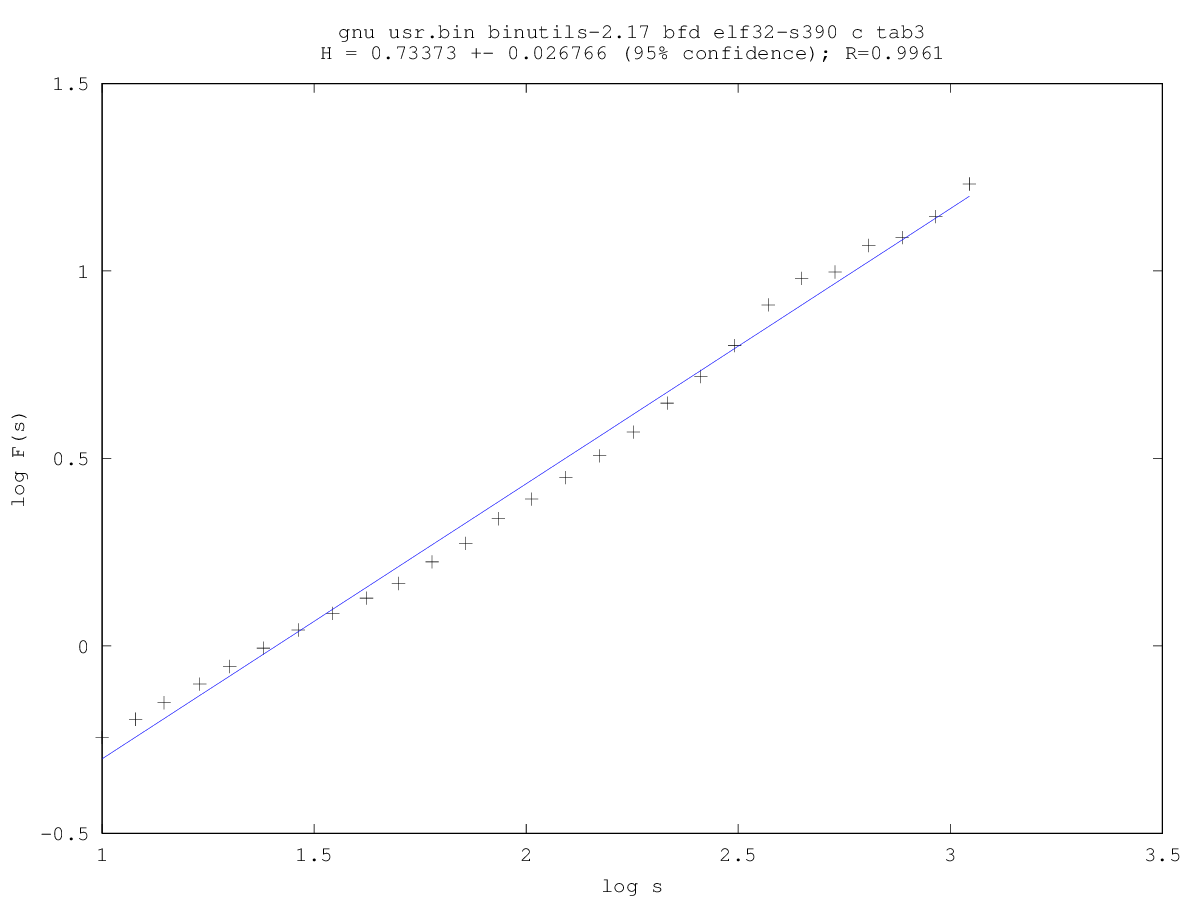
\includegraphics[width=0.8\linewidth]{{fractals/data/gnu_usr.bin_binutils-2.17_bfd_elf32-s390_c_tab3_log_log}.png}
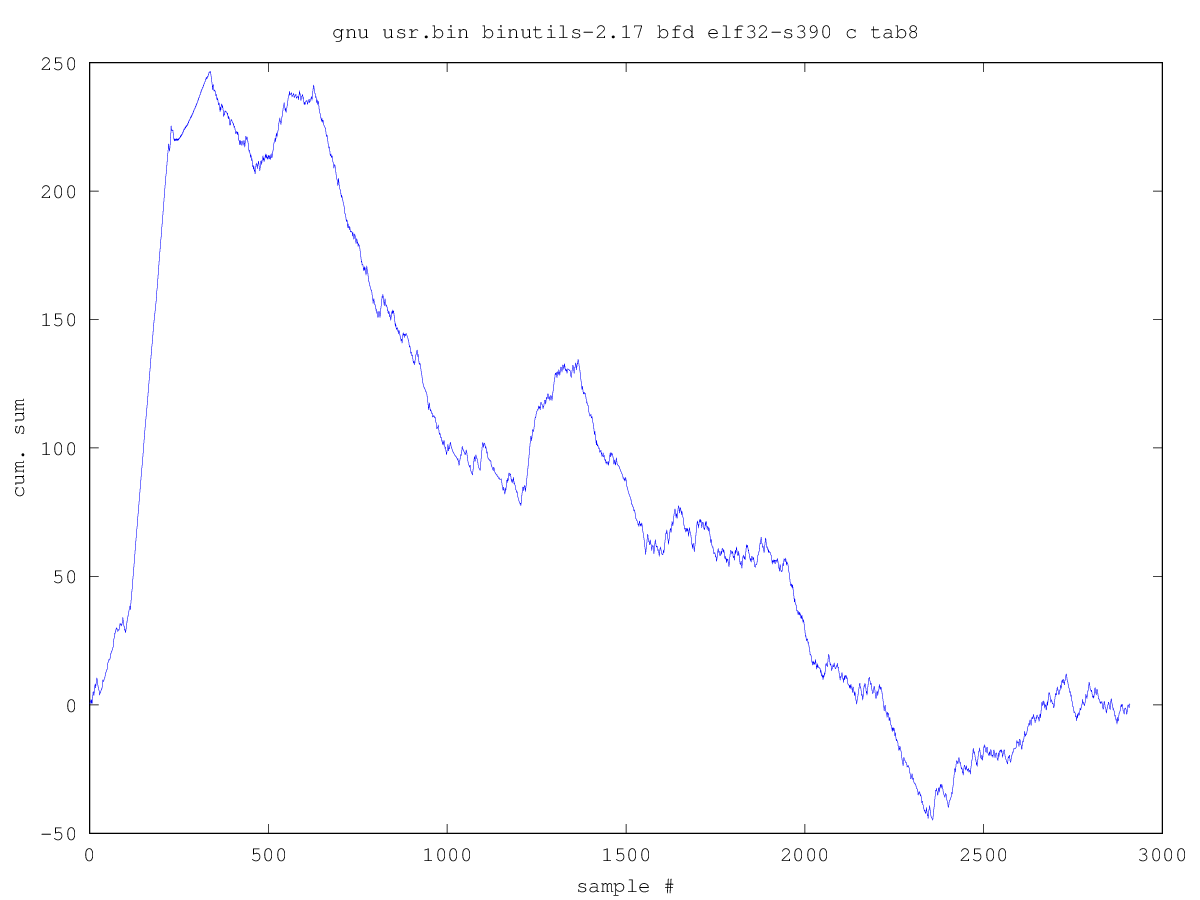
\includegraphics[width=0.8\linewidth]{{fractals/data/gnu_usr.bin_binutils-2.17_bfd_elf32-s390_c_tab8_time_series}.png}
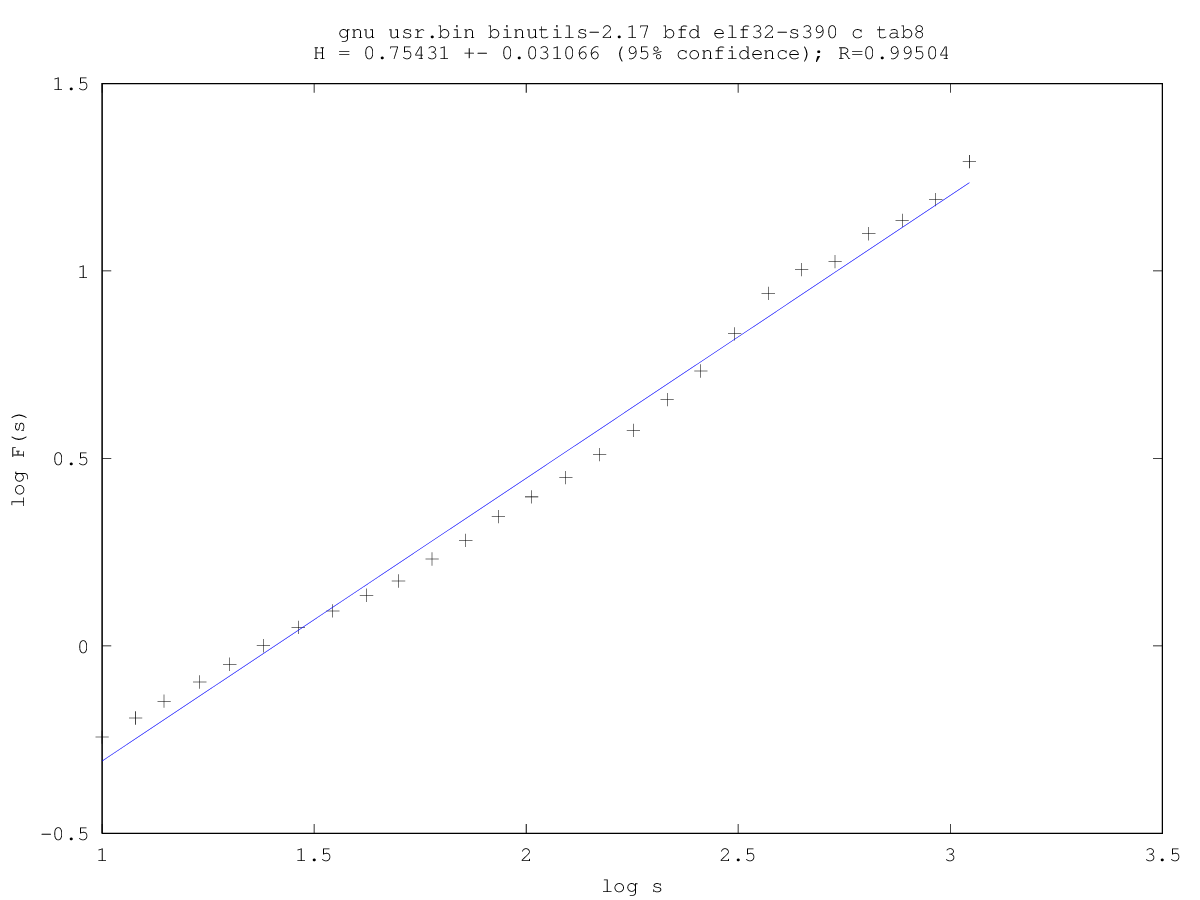
\includegraphics[width=0.8\linewidth]{{fractals/data/gnu_usr.bin_binutils-2.17_bfd_elf32-s390_c_tab8_log_log}.png}
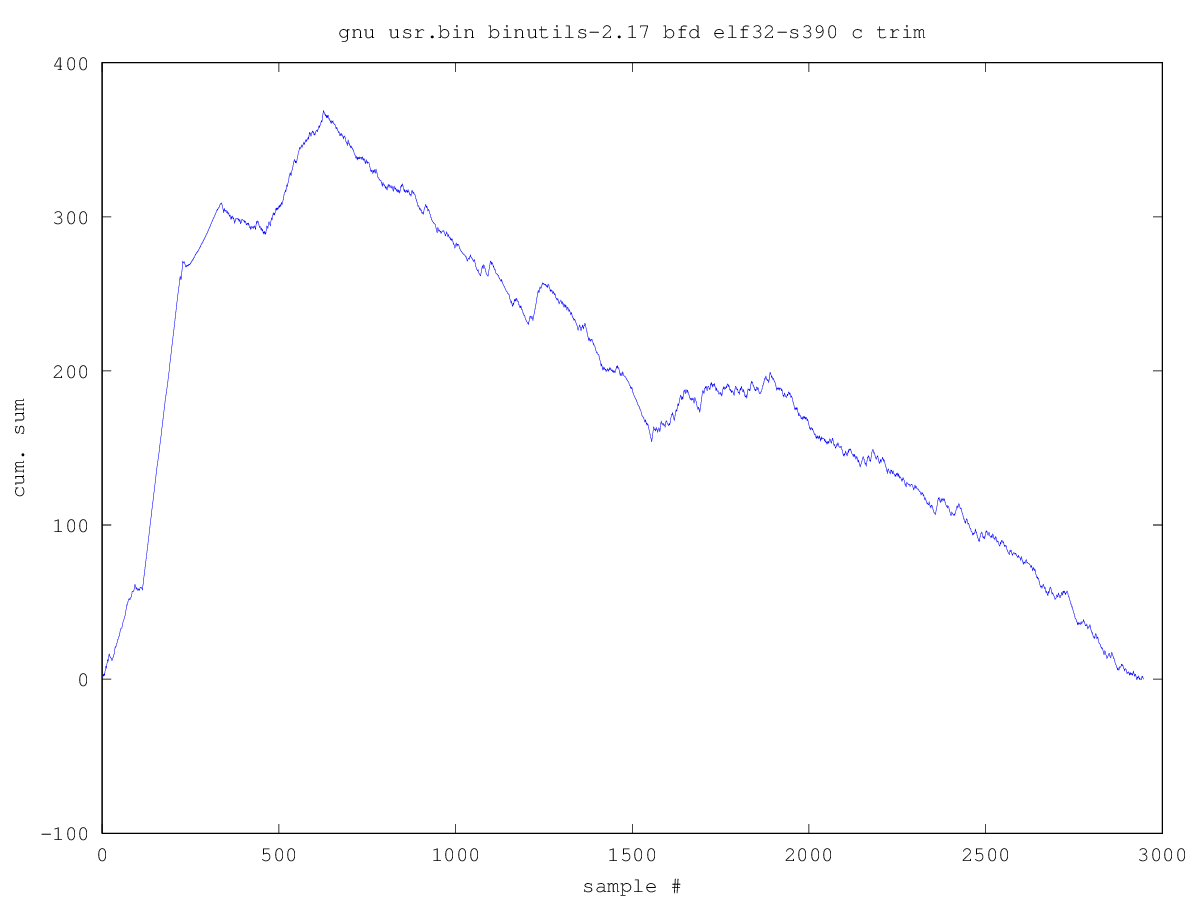
\includegraphics[width=0.8\linewidth]{{fractals/data/gnu_usr.bin_binutils-2.17_bfd_elf32-s390_c_trim_time_series}.png}
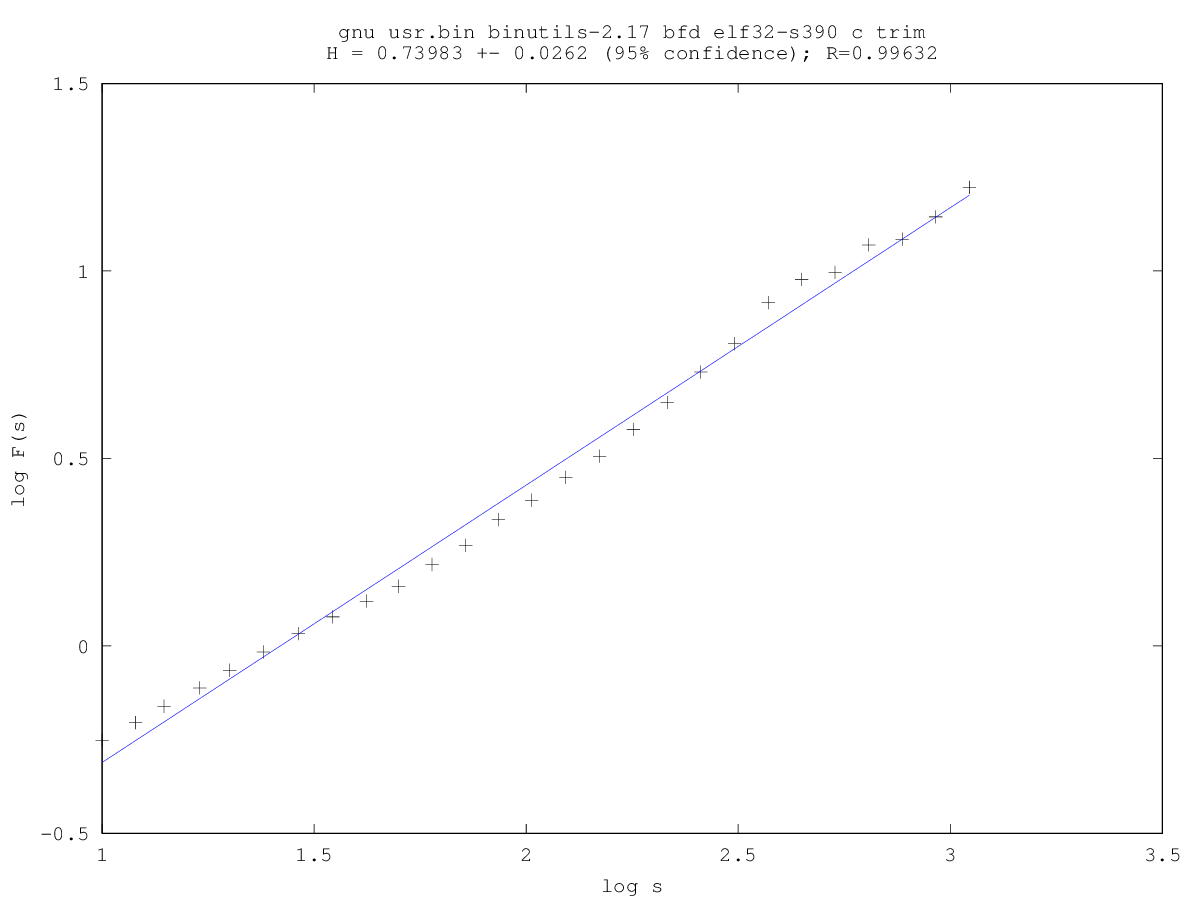
\includegraphics[width=0.8\linewidth]{{fractals/data/gnu_usr.bin_binutils-2.17_bfd_elf32-s390_c_trim_log_log}.png}
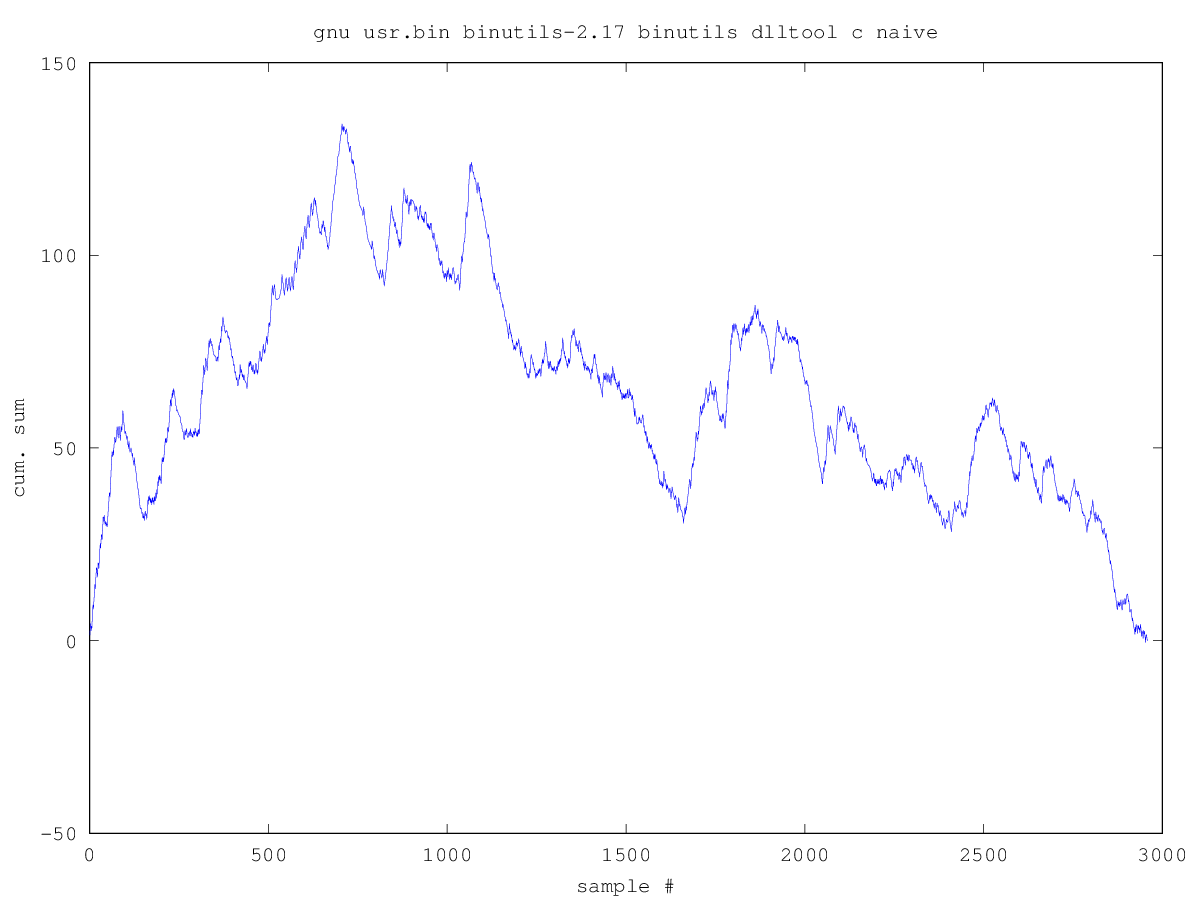
\includegraphics[width=0.8\linewidth]{{fractals/data/gnu_usr.bin_binutils-2.17_binutils_dlltool_c_naive_time_series}.png}
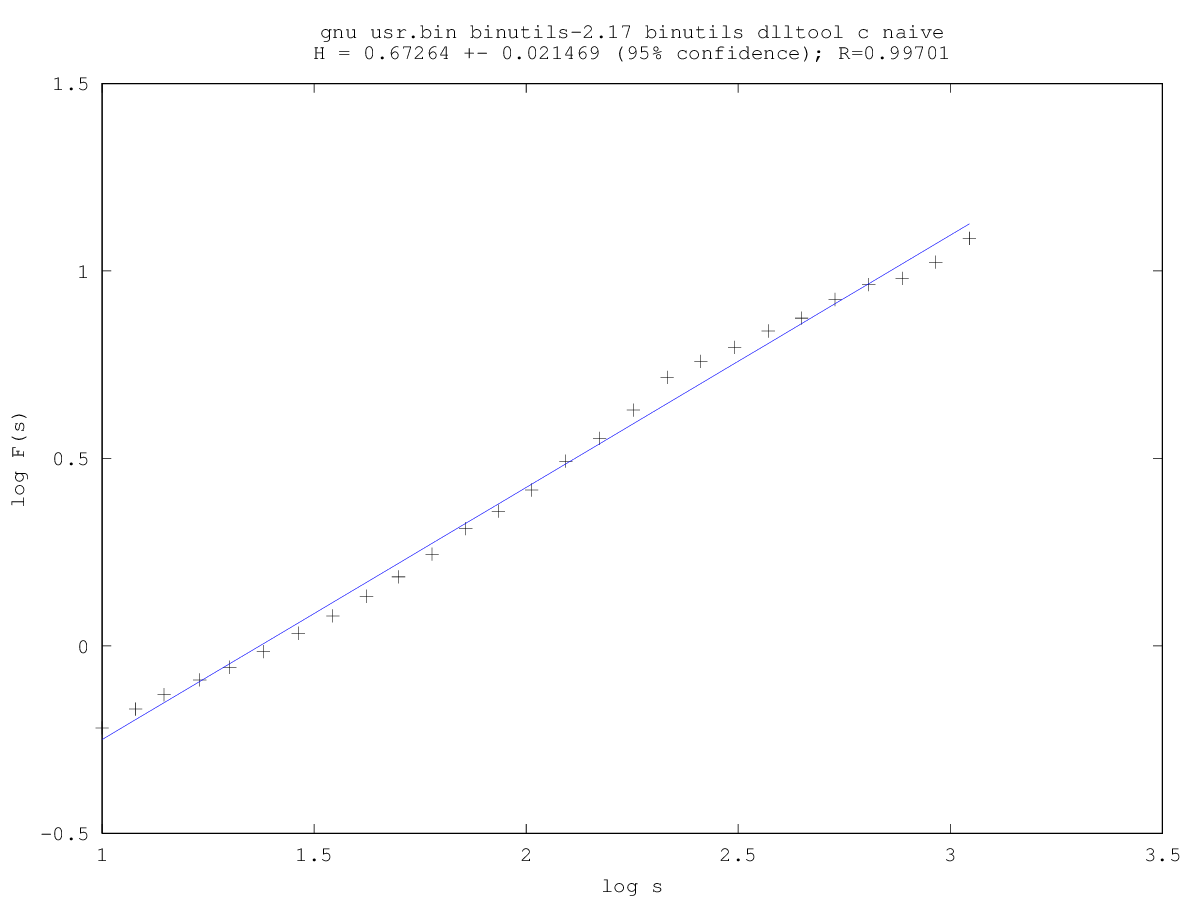
\includegraphics[width=0.8\linewidth]{{fractals/data/gnu_usr.bin_binutils-2.17_binutils_dlltool_c_naive_log_log}.png}
\includegraphics[width=0.8\linewidth]{{fractals/data/gnu_usr.bin_binutils-2.17_binutils_dlltool_c_tab3_time_series}.png}
\includegraphics[width=0.8\linewidth]{{fractals/data/gnu_usr.bin_binutils-2.17_binutils_dlltool_c_tab3_log_log}.png}
\includegraphics[width=0.8\linewidth]{{fractals/data/gnu_usr.bin_binutils-2.17_binutils_dlltool_c_tab8_time_series}.png}
\includegraphics[width=0.8\linewidth]{{fractals/data/gnu_usr.bin_binutils-2.17_binutils_dlltool_c_tab8_log_log}.png}
\includegraphics[width=0.8\linewidth]{{fractals/data/gnu_usr.bin_binutils-2.17_binutils_dlltool_c_trim_time_series}.png}
\includegraphics[width=0.8\linewidth]{{fractals/data/gnu_usr.bin_binutils-2.17_binutils_dlltool_c_trim_log_log}.png}
\includegraphics[width=0.8\linewidth]{{fractals/data/gnu_usr.bin_binutils-2.17_gas_config_tc-sh64_c_naive_time_series}.png}
\includegraphics[width=0.8\linewidth]{{fractals/data/gnu_usr.bin_binutils-2.17_gas_config_tc-sh64_c_naive_log_log}.png}
\includegraphics[width=0.8\linewidth]{{fractals/data/gnu_usr.bin_binutils-2.17_gas_config_tc-sh64_c_tab3_time_series}.png}
\includegraphics[width=0.8\linewidth]{{fractals/data/gnu_usr.bin_binutils-2.17_gas_config_tc-sh64_c_tab3_log_log}.png}
\includegraphics[width=0.8\linewidth]{{fractals/data/gnu_usr.bin_binutils-2.17_gas_config_tc-sh64_c_tab8_time_series}.png}
\includegraphics[width=0.8\linewidth]{{fractals/data/gnu_usr.bin_binutils-2.17_gas_config_tc-sh64_c_tab8_log_log}.png}
\includegraphics[width=0.8\linewidth]{{fractals/data/gnu_usr.bin_binutils-2.17_gas_config_tc-sh64_c_trim_time_series}.png}
\includegraphics[width=0.8\linewidth]{{fractals/data/gnu_usr.bin_binutils-2.17_gas_config_tc-sh64_c_trim_log_log}.png}
\includegraphics[width=0.8\linewidth]{{fractals/data/gnu_usr.bin_binutils-2.17_opcodes_xc16x-desc_c_naive_time_series}.png}
\includegraphics[width=0.8\linewidth]{{fractals/data/gnu_usr.bin_binutils-2.17_opcodes_xc16x-desc_c_naive_log_log}.png}
\includegraphics[width=0.8\linewidth]{{fractals/data/gnu_usr.bin_binutils-2.17_opcodes_xc16x-desc_c_tab3_time_series}.png}
\includegraphics[width=0.8\linewidth]{{fractals/data/gnu_usr.bin_binutils-2.17_opcodes_xc16x-desc_c_tab3_log_log}.png}
\includegraphics[width=0.8\linewidth]{{fractals/data/gnu_usr.bin_binutils-2.17_opcodes_xc16x-desc_c_tab8_time_series}.png}
\includegraphics[width=0.8\linewidth]{{fractals/data/gnu_usr.bin_binutils-2.17_opcodes_xc16x-desc_c_tab8_log_log}.png}
\includegraphics[width=0.8\linewidth]{{fractals/data/gnu_usr.bin_binutils-2.17_opcodes_xc16x-desc_c_trim_time_series}.png}
\includegraphics[width=0.8\linewidth]{{fractals/data/gnu_usr.bin_binutils-2.17_opcodes_xc16x-desc_c_trim_log_log}.png}
\includegraphics[width=0.8\linewidth]{{fractals/data/gnu_usr.bin_binutils_binutils_rcparse_c_naive_time_series}.png}
\includegraphics[width=0.8\linewidth]{{fractals/data/gnu_usr.bin_binutils_binutils_rcparse_c_naive_log_log}.png}
\includegraphics[width=0.8\linewidth]{{fractals/data/gnu_usr.bin_binutils_binutils_rcparse_c_tab3_time_series}.png}
\includegraphics[width=0.8\linewidth]{{fractals/data/gnu_usr.bin_binutils_binutils_rcparse_c_tab3_log_log}.png}
\includegraphics[width=0.8\linewidth]{{fractals/data/gnu_usr.bin_binutils_binutils_rcparse_c_tab8_time_series}.png}
\includegraphics[width=0.8\linewidth]{{fractals/data/gnu_usr.bin_binutils_binutils_rcparse_c_tab8_log_log}.png}
\includegraphics[width=0.8\linewidth]{{fractals/data/gnu_usr.bin_binutils_binutils_rcparse_c_trim_time_series}.png}
\includegraphics[width=0.8\linewidth]{{fractals/data/gnu_usr.bin_binutils_binutils_rcparse_c_trim_log_log}.png}
\includegraphics[width=0.8\linewidth]{{fractals/data/gnu_usr.bin_binutils_gas_config_tc-sh64_c_naive_time_series}.png}
\includegraphics[width=0.8\linewidth]{{fractals/data/gnu_usr.bin_binutils_gas_config_tc-sh64_c_naive_log_log}.png}
\includegraphics[width=0.8\linewidth]{{fractals/data/gnu_usr.bin_binutils_gas_config_tc-sh64_c_tab3_time_series}.png}
\includegraphics[width=0.8\linewidth]{{fractals/data/gnu_usr.bin_binutils_gas_config_tc-sh64_c_tab3_log_log}.png}
\includegraphics[width=0.8\linewidth]{{fractals/data/gnu_usr.bin_binutils_gas_config_tc-sh64_c_tab8_time_series}.png}
\includegraphics[width=0.8\linewidth]{{fractals/data/gnu_usr.bin_binutils_gas_config_tc-sh64_c_tab8_log_log}.png}
\includegraphics[width=0.8\linewidth]{{fractals/data/gnu_usr.bin_binutils_gas_config_tc-sh64_c_trim_time_series}.png}
\includegraphics[width=0.8\linewidth]{{fractals/data/gnu_usr.bin_binutils_gas_config_tc-sh64_c_trim_log_log}.png}
\includegraphics[width=0.8\linewidth]{{fractals/data/gnu_usr.bin_gcc_gcc_config_d30v_d30v_c_naive_time_series}.png}
\includegraphics[width=0.8\linewidth]{{fractals/data/gnu_usr.bin_gcc_gcc_config_d30v_d30v_c_naive_log_log}.png}
\includegraphics[width=0.8\linewidth]{{fractals/data/gnu_usr.bin_gcc_gcc_config_d30v_d30v_c_tab3_time_series}.png}
\includegraphics[width=0.8\linewidth]{{fractals/data/gnu_usr.bin_gcc_gcc_config_d30v_d30v_c_tab3_log_log}.png}
\includegraphics[width=0.8\linewidth]{{fractals/data/gnu_usr.bin_gcc_gcc_config_d30v_d30v_c_tab8_time_series}.png}
\includegraphics[width=0.8\linewidth]{{fractals/data/gnu_usr.bin_gcc_gcc_config_d30v_d30v_c_tab8_log_log}.png}
\includegraphics[width=0.8\linewidth]{{fractals/data/gnu_usr.bin_gcc_gcc_config_d30v_d30v_c_trim_time_series}.png}
\includegraphics[width=0.8\linewidth]{{fractals/data/gnu_usr.bin_gcc_gcc_config_d30v_d30v_c_trim_log_log}.png}
\includegraphics[width=0.8\linewidth]{{fractals/data/gnu_usr.bin_gcc_gcc_config_mcore_mcore_c_naive_time_series}.png}
\includegraphics[width=0.8\linewidth]{{fractals/data/gnu_usr.bin_gcc_gcc_config_mcore_mcore_c_naive_log_log}.png}
\includegraphics[width=0.8\linewidth]{{fractals/data/gnu_usr.bin_gcc_gcc_config_mcore_mcore_c_tab3_time_series}.png}
\includegraphics[width=0.8\linewidth]{{fractals/data/gnu_usr.bin_gcc_gcc_config_mcore_mcore_c_tab3_log_log}.png}
\includegraphics[width=0.8\linewidth]{{fractals/data/gnu_usr.bin_gcc_gcc_config_mcore_mcore_c_tab8_time_series}.png}
\includegraphics[width=0.8\linewidth]{{fractals/data/gnu_usr.bin_gcc_gcc_config_mcore_mcore_c_tab8_log_log}.png}
\includegraphics[width=0.8\linewidth]{{fractals/data/gnu_usr.bin_gcc_gcc_config_mcore_mcore_c_trim_time_series}.png}
\includegraphics[width=0.8\linewidth]{{fractals/data/gnu_usr.bin_gcc_gcc_config_mcore_mcore_c_trim_log_log}.png}
\includegraphics[width=0.8\linewidth]{{fractals/data/gnu_usr.bin_gcc_gcc_java_expr_c_naive_time_series}.png}
\includegraphics[width=0.8\linewidth]{{fractals/data/gnu_usr.bin_gcc_gcc_java_expr_c_naive_log_log}.png}
\includegraphics[width=0.8\linewidth]{{fractals/data/gnu_usr.bin_gcc_gcc_java_expr_c_tab3_time_series}.png}
\includegraphics[width=0.8\linewidth]{{fractals/data/gnu_usr.bin_gcc_gcc_java_expr_c_tab3_log_log}.png}
\includegraphics[width=0.8\linewidth]{{fractals/data/gnu_usr.bin_gcc_gcc_java_expr_c_tab8_time_series}.png}
\includegraphics[width=0.8\linewidth]{{fractals/data/gnu_usr.bin_gcc_gcc_java_expr_c_tab8_log_log}.png}
\includegraphics[width=0.8\linewidth]{{fractals/data/gnu_usr.bin_gcc_gcc_java_expr_c_trim_time_series}.png}
\includegraphics[width=0.8\linewidth]{{fractals/data/gnu_usr.bin_gcc_gcc_java_expr_c_trim_log_log}.png}
\includegraphics[width=0.8\linewidth]{{fractals/data/gnu_usr.bin_gcc_gcc_recog_c_naive_time_series}.png}
\includegraphics[width=0.8\linewidth]{{fractals/data/gnu_usr.bin_gcc_gcc_recog_c_naive_log_log}.png}
\includegraphics[width=0.8\linewidth]{{fractals/data/gnu_usr.bin_gcc_gcc_recog_c_tab3_time_series}.png}
\includegraphics[width=0.8\linewidth]{{fractals/data/gnu_usr.bin_gcc_gcc_recog_c_tab3_log_log}.png}
\includegraphics[width=0.8\linewidth]{{fractals/data/gnu_usr.bin_gcc_gcc_recog_c_tab8_time_series}.png}
\includegraphics[width=0.8\linewidth]{{fractals/data/gnu_usr.bin_gcc_gcc_recog_c_tab8_log_log}.png}
\includegraphics[width=0.8\linewidth]{{fractals/data/gnu_usr.bin_gcc_gcc_recog_c_trim_time_series}.png}
\includegraphics[width=0.8\linewidth]{{fractals/data/gnu_usr.bin_gcc_gcc_recog_c_trim_log_log}.png}
\includegraphics[width=0.8\linewidth]{{fractals/data/gnu_usr.bin_perl_hv_c_naive_time_series}.png}
\includegraphics[width=0.8\linewidth]{{fractals/data/gnu_usr.bin_perl_hv_c_naive_log_log}.png}
\includegraphics[width=0.8\linewidth]{{fractals/data/gnu_usr.bin_perl_hv_c_tab3_time_series}.png}
\includegraphics[width=0.8\linewidth]{{fractals/data/gnu_usr.bin_perl_hv_c_tab3_log_log}.png}
\includegraphics[width=0.8\linewidth]{{fractals/data/gnu_usr.bin_perl_hv_c_tab8_time_series}.png}
\includegraphics[width=0.8\linewidth]{{fractals/data/gnu_usr.bin_perl_hv_c_tab8_log_log}.png}
\includegraphics[width=0.8\linewidth]{{fractals/data/gnu_usr.bin_perl_hv_c_trim_time_series}.png}
\includegraphics[width=0.8\linewidth]{{fractals/data/gnu_usr.bin_perl_hv_c_trim_log_log}.png}
\includegraphics[width=0.8\linewidth]{{fractals/data/lib_libpcap_gencode_c_naive_time_series}.png}
\includegraphics[width=0.8\linewidth]{{fractals/data/lib_libpcap_gencode_c_naive_log_log}.png}
\includegraphics[width=0.8\linewidth]{{fractals/data/lib_libpcap_gencode_c_tab3_time_series}.png}
\includegraphics[width=0.8\linewidth]{{fractals/data/lib_libpcap_gencode_c_tab3_log_log}.png}
\includegraphics[width=0.8\linewidth]{{fractals/data/lib_libpcap_gencode_c_tab8_time_series}.png}
\includegraphics[width=0.8\linewidth]{{fractals/data/lib_libpcap_gencode_c_tab8_log_log}.png}
\includegraphics[width=0.8\linewidth]{{fractals/data/lib_libpcap_gencode_c_trim_time_series}.png}
\includegraphics[width=0.8\linewidth]{{fractals/data/lib_libpcap_gencode_c_trim_log_log}.png}
\includegraphics[width=0.8\linewidth]{{fractals/data/sys_arch_arm_arm_pmap7_c_naive_time_series}.png}
\includegraphics[width=0.8\linewidth]{{fractals/data/sys_arch_arm_arm_pmap7_c_naive_log_log}.png}
\includegraphics[width=0.8\linewidth]{{fractals/data/sys_arch_arm_arm_pmap7_c_tab3_time_series}.png}
\includegraphics[width=0.8\linewidth]{{fractals/data/sys_arch_arm_arm_pmap7_c_tab3_log_log}.png}
\includegraphics[width=0.8\linewidth]{{fractals/data/sys_arch_arm_arm_pmap7_c_tab8_time_series}.png}
\includegraphics[width=0.8\linewidth]{{fractals/data/sys_arch_arm_arm_pmap7_c_tab8_log_log}.png}
\includegraphics[width=0.8\linewidth]{{fractals/data/sys_arch_arm_arm_pmap7_c_trim_time_series}.png}
\includegraphics[width=0.8\linewidth]{{fractals/data/sys_arch_arm_arm_pmap7_c_trim_log_log}.png}
\includegraphics[width=0.8\linewidth]{{fractals/data/sys_dev_audio_c_naive_time_series}.png}
\includegraphics[width=0.8\linewidth]{{fractals/data/sys_dev_audio_c_naive_log_log}.png}
\includegraphics[width=0.8\linewidth]{{fractals/data/sys_dev_audio_c_tab3_time_series}.png}
\includegraphics[width=0.8\linewidth]{{fractals/data/sys_dev_audio_c_tab3_log_log}.png}
\includegraphics[width=0.8\linewidth]{{fractals/data/sys_dev_audio_c_tab8_time_series}.png}
\includegraphics[width=0.8\linewidth]{{fractals/data/sys_dev_audio_c_tab8_log_log}.png}
\includegraphics[width=0.8\linewidth]{{fractals/data/sys_dev_audio_c_trim_time_series}.png}
\includegraphics[width=0.8\linewidth]{{fractals/data/sys_dev_audio_c_trim_log_log}.png}
\includegraphics[width=0.8\linewidth]{{fractals/data/sys_dev_ic_mpi_c_naive_time_series}.png}
\includegraphics[width=0.8\linewidth]{{fractals/data/sys_dev_ic_mpi_c_naive_log_log}.png}
\includegraphics[width=0.8\linewidth]{{fractals/data/sys_dev_ic_mpi_c_tab3_time_series}.png}
\includegraphics[width=0.8\linewidth]{{fractals/data/sys_dev_ic_mpi_c_tab3_log_log}.png}
\includegraphics[width=0.8\linewidth]{{fractals/data/sys_dev_ic_mpi_c_tab8_time_series}.png}
\includegraphics[width=0.8\linewidth]{{fractals/data/sys_dev_ic_mpi_c_tab8_log_log}.png}
\includegraphics[width=0.8\linewidth]{{fractals/data/sys_dev_ic_mpi_c_trim_time_series}.png}
\includegraphics[width=0.8\linewidth]{{fractals/data/sys_dev_ic_mpi_c_trim_log_log}.png}
\includegraphics[width=0.8\linewidth]{{fractals/data/sys_dev_isa_gus_c_naive_time_series}.png}
\includegraphics[width=0.8\linewidth]{{fractals/data/sys_dev_isa_gus_c_naive_log_log}.png}
\includegraphics[width=0.8\linewidth]{{fractals/data/sys_dev_isa_gus_c_tab3_time_series}.png}
\includegraphics[width=0.8\linewidth]{{fractals/data/sys_dev_isa_gus_c_tab3_log_log}.png}
\includegraphics[width=0.8\linewidth]{{fractals/data/sys_dev_isa_gus_c_tab8_time_series}.png}
\includegraphics[width=0.8\linewidth]{{fractals/data/sys_dev_isa_gus_c_tab8_log_log}.png}
\includegraphics[width=0.8\linewidth]{{fractals/data/sys_dev_isa_gus_c_trim_time_series}.png}
\includegraphics[width=0.8\linewidth]{{fractals/data/sys_dev_isa_gus_c_trim_log_log}.png}
\includegraphics[width=0.8\linewidth]{{fractals/data/sys_dev_pci_if_oce_c_naive_time_series}.png}
\includegraphics[width=0.8\linewidth]{{fractals/data/sys_dev_pci_if_oce_c_naive_log_log}.png}
\includegraphics[width=0.8\linewidth]{{fractals/data/sys_dev_pci_if_oce_c_tab3_time_series}.png}
\includegraphics[width=0.8\linewidth]{{fractals/data/sys_dev_pci_if_oce_c_tab3_log_log}.png}
\includegraphics[width=0.8\linewidth]{{fractals/data/sys_dev_pci_if_oce_c_tab8_time_series}.png}
\includegraphics[width=0.8\linewidth]{{fractals/data/sys_dev_pci_if_oce_c_tab8_log_log}.png}
\includegraphics[width=0.8\linewidth]{{fractals/data/sys_dev_pci_if_oce_c_trim_time_series}.png}
\includegraphics[width=0.8\linewidth]{{fractals/data/sys_dev_pci_if_oce_c_trim_log_log}.png}
\includegraphics[width=0.8\linewidth]{{fractals/data/sys_dev_pci_if_san_xilinx_c_naive_time_series}.png}
\includegraphics[width=0.8\linewidth]{{fractals/data/sys_dev_pci_if_san_xilinx_c_naive_log_log}.png}
\includegraphics[width=0.8\linewidth]{{fractals/data/sys_dev_pci_if_san_xilinx_c_tab3_time_series}.png}
\includegraphics[width=0.8\linewidth]{{fractals/data/sys_dev_pci_if_san_xilinx_c_tab3_log_log}.png}
\includegraphics[width=0.8\linewidth]{{fractals/data/sys_dev_pci_if_san_xilinx_c_tab8_time_series}.png}
\includegraphics[width=0.8\linewidth]{{fractals/data/sys_dev_pci_if_san_xilinx_c_tab8_log_log}.png}
\includegraphics[width=0.8\linewidth]{{fractals/data/sys_dev_pci_if_san_xilinx_c_trim_time_series}.png}
\includegraphics[width=0.8\linewidth]{{fractals/data/sys_dev_pci_if_san_xilinx_c_trim_log_log}.png}
\includegraphics[width=0.8\linewidth]{{fractals/data/usr.sbin_bgpd_rde_c_naive_time_series}.png}
\includegraphics[width=0.8\linewidth]{{fractals/data/usr.sbin_bgpd_rde_c_naive_log_log}.png}
\includegraphics[width=0.8\linewidth]{{fractals/data/usr.sbin_bgpd_rde_c_tab3_time_series}.png}
\includegraphics[width=0.8\linewidth]{{fractals/data/usr.sbin_bgpd_rde_c_tab3_log_log}.png}
\includegraphics[width=0.8\linewidth]{{fractals/data/usr.sbin_bgpd_rde_c_tab8_time_series}.png}
\includegraphics[width=0.8\linewidth]{{fractals/data/usr.sbin_bgpd_rde_c_tab8_log_log}.png}
\includegraphics[width=0.8\linewidth]{{fractals/data/usr.sbin_bgpd_rde_c_trim_time_series}.png}
\includegraphics[width=0.8\linewidth]{{fractals/data/usr.sbin_bgpd_rde_c_trim_log_log}.png}
\includegraphics[width=0.8\linewidth]{{fractals/data/usr.sbin_nginx_src_http_modules_ngx_http_mp4_module_c_naive_time_series}.png}
\includegraphics[width=0.8\linewidth]{{fractals/data/usr.sbin_nginx_src_http_modules_ngx_http_mp4_module_c_naive_log_log}.png}
\includegraphics[width=0.8\linewidth]{{fractals/data/usr.sbin_nginx_src_http_modules_ngx_http_mp4_module_c_tab3_time_series}.png}
\includegraphics[width=0.8\linewidth]{{fractals/data/usr.sbin_nginx_src_http_modules_ngx_http_mp4_module_c_tab3_log_log}.png}
\includegraphics[width=0.8\linewidth]{{fractals/data/usr.sbin_nginx_src_http_modules_ngx_http_mp4_module_c_tab8_time_series}.png}
\includegraphics[width=0.8\linewidth]{{fractals/data/usr.sbin_nginx_src_http_modules_ngx_http_mp4_module_c_tab8_log_log}.png}
\includegraphics[width=0.8\linewidth]{{fractals/data/usr.sbin_nginx_src_http_modules_ngx_http_mp4_module_c_trim_time_series}.png}
\includegraphics[width=0.8\linewidth]{{fractals/data/usr.sbin_nginx_src_http_modules_ngx_http_mp4_module_c_trim_log_log}.png}

\end{center}


%\section{Full Results - Other Languages}\label{FullResultsOther}
%\label{FullResultsOther}
\subsection{Table - DFA2 Analysis results per source file}
TODO cite these
\begin{longtable}{l l r r r}
\textbf{Filename} & \textbf{Type} & \textbf{H} & \textbf{+/-} & \textbf{R} \\
{jquery-1.11.1.js} & naive & 0.58557 & 0.010196 & 0.99911 \\
{jquery-1.11.1.js} & trim & 0.58759 & 0.010714 & 0.99902 \\
{message.rb} & trim & 0.5677 & 0.01124 & 0.99885 \\
{jquery-1.11.1.js} & tab3 & 0.61124 & 0.01249 & 0.99877 \\
{message.rb} & naive & 0.56266 & 0.012069 & 0.99865 \\
{message.rb} & tab3 & 0.56266 & 0.012069 & 0.99865 \\
{message.rb} & tab8 & 0.56266 & 0.012069 & 0.99865 \\
{StorageService.java} & tab8 & 0.67267 & 0.01641 & 0.99825 \\
{StorageService.java} & naive & 0.6721 & 0.016419 & 0.99825 \\
{StorageService.java} & tab3 & 0.67223 & 0.016457 & 0.99824 \\
{jquery-1.11.1.js} & tab8 & 0.72399 & 0.019735 & 0.99782 \\
{StorageService.java} & trim & 0.61487 & 0.022114 & 0.99621 \\
{BigInteger.cs} & trim & 0.70561 & 0.025801 & 0.99608 \\
{BigInteger.cs} & naive & 0.70258 & 0.028364 & 0.99523 \\
{BigInteger.cs} & tab3 & 0.70918 & 0.033326 & 0.99356 \\
{tests.py} & tab8 & 0.58898 & 0.029061 & 0.9929 \\
{tests.py} & naive & 0.58898 & 0.029061 & 0.9929 \\
{tests.py} & tab3 & 0.58898 & 0.029061 & 0.9929 \\
{tests.py} & trim & 0.63369 & 0.032319 & 0.99242 \\
{activerecord.html} & naive & 0.4035 & 0.021247 & 0.99193 \\
{activerecord.html} & tab3 & 0.4035 & 0.021247 & 0.99193 \\
{activerecord.html} & tab8 & 0.4035 & 0.021247 & 0.99193 \\
{BigInteger.cs} & tab8 & 0.74006 & 0.043006 & 0.99019 \\
{activerecord.html} & trim & 0.40015 & 0.027494 & 0.98637 \\
\end{longtable}

\newpage
\subsection{Table - DFA2 Variance - Other Languages}\label{FullResultsOtherVariance}
\begin{longtable}{l r}
\textbf{Filename} &  \textbf{H} \\
{activerecord.html} & 0.0033500000000000196  \\
{BigInteger.cs} & 0.03748000000000007  \\
{jquery-1.11.1.js} & 0.13842  \\
{message.rb} & 0.005039999999999933  \\
{StorageService.java} & 0.05779999999999996  \\
{tests.py} & 0.04471000000000003  \\
\end{longtable}
\begin{longtable}{l r}
\textbf{Filename} &  \textbf{+/-} \\
{activerecord.html} & 0.0062470000000000026  \\
{BigInteger.cs} & 0.017205  \\
{jquery-1.11.1.js} & 0.009538999999999999  \\
{message.rb} & 0.0008289999999999999  \\
{StorageService.java} & 0.005704000000000001  \\
{tests.py} & 0.0032580000000000005  \\
\end{longtable}
\begin{longtable}{l r}
\textbf{Filename} &  \textbf{R} \\
{activerecord.html} & 0.005560000000000009  \\
{BigInteger.cs} & 0.005889999999999951  \\
{jquery-1.11.1.js} & 0.0012900000000000134  \\
{message.rb} & 0.00019999999999997797  \\
{StorageService.java} & 0.0020399999999999308  \\
{tests.py} & 0.00048000000000003595  \\
\end{longtable}

\newpage
\subsection{Graphs - Other Languages}
\begin{center}
\includegraphics[width=0.8\linewidth]{{fractals/other_lang_data/other_langs_BigInteger_cs_naive_time_series}.png}
\includegraphics[width=0.8\linewidth]{{fractals/other_lang_data/other_langs_BigInteger_cs_naive_log_log}.png}
\includegraphics[width=0.8\linewidth]{{fractals/other_lang_data/other_langs_BigInteger_cs_tab3_time_series}.png}
\includegraphics[width=0.8\linewidth]{{fractals/other_lang_data/other_langs_BigInteger_cs_tab3_log_log}.png}
\includegraphics[width=0.8\linewidth]{{fractals/other_lang_data/other_langs_BigInteger_cs_tab8_time_series}.png}
\includegraphics[width=0.8\linewidth]{{fractals/other_lang_data/other_langs_BigInteger_cs_tab8_log_log}.png}
\includegraphics[width=0.8\linewidth]{{fractals/other_lang_data/other_langs_BigInteger_cs_trim_time_series}.png}
\includegraphics[width=0.8\linewidth]{{fractals/other_lang_data/other_langs_BigInteger_cs_trim_log_log}.png}
\includegraphics[width=0.8\linewidth]{{fractals/other_lang_data/other_langs_StorageService.java_naive_time_series}.png}
\includegraphics[width=0.8\linewidth]{{fractals/other_lang_data/other_langs_StorageService.java_naive_log_log}.png}
\includegraphics[width=0.8\linewidth]{{fractals/other_lang_data/other_langs_StorageService.java_tab3_time_series}.png}
\includegraphics[width=0.8\linewidth]{{fractals/other_lang_data/other_langs_StorageService.java_tab3_log_log}.png}
\includegraphics[width=0.8\linewidth]{{fractals/other_lang_data/other_langs_StorageService.java_tab8_time_series}.png}
\includegraphics[width=0.8\linewidth]{{fractals/other_lang_data/other_langs_StorageService.java_tab8_log_log}.png}
\includegraphics[width=0.8\linewidth]{{fractals/other_lang_data/other_langs_StorageService.java_trim_time_series}.png}
\includegraphics[width=0.8\linewidth]{{fractals/other_lang_data/other_langs_StorageService.java_trim_log_log}.png}
\includegraphics[width=0.8\linewidth]{{fractals/other_lang_data/other_langs_activerecord.html_naive_time_series}.png}
\includegraphics[width=0.8\linewidth]{{fractals/other_lang_data/other_langs_activerecord.html_naive_log_log}.png}
\includegraphics[width=0.8\linewidth]{{fractals/other_lang_data/other_langs_activerecord.html_tab3_time_series}.png}
\includegraphics[width=0.8\linewidth]{{fractals/other_lang_data/other_langs_activerecord.html_tab3_log_log}.png}
\includegraphics[width=0.8\linewidth]{{fractals/other_lang_data/other_langs_activerecord.html_tab8_time_series}.png}
\includegraphics[width=0.8\linewidth]{{fractals/other_lang_data/other_langs_activerecord.html_tab8_log_log}.png}
\includegraphics[width=0.8\linewidth]{{fractals/other_lang_data/other_langs_activerecord.html_trim_time_series}.png}
\includegraphics[width=0.8\linewidth]{{fractals/other_lang_data/other_langs_activerecord.html_trim_log_log}.png}
\includegraphics[width=0.8\linewidth]{{fractals/other_lang_data/other_langs_jquery-1.11.1.js_naive_time_series}.png}
\includegraphics[width=0.8\linewidth]{{fractals/other_lang_data/other_langs_jquery-1.11.1.js_naive_log_log}.png}
\includegraphics[width=0.8\linewidth]{{fractals/other_lang_data/other_langs_jquery-1.11.1.js_tab3_time_series}.png}
\includegraphics[width=0.8\linewidth]{{fractals/other_lang_data/other_langs_jquery-1.11.1.js_tab3_log_log}.png}
\includegraphics[width=0.8\linewidth]{{fractals/other_lang_data/other_langs_jquery-1.11.1.js_tab8_time_series}.png}
\includegraphics[width=0.8\linewidth]{{fractals/other_lang_data/other_langs_jquery-1.11.1.js_tab8_log_log}.png}
\includegraphics[width=0.8\linewidth]{{fractals/other_lang_data/other_langs_jquery-1.11.1.js_trim_time_series}.png}
\includegraphics[width=0.8\linewidth]{{fractals/other_lang_data/other_langs_jquery-1.11.1.js_trim_log_log}.png}
\includegraphics[width=0.8\linewidth]{{fractals/other_lang_data/other_langs_message.rb_naive_time_series}.png}
\includegraphics[width=0.8\linewidth]{{fractals/other_lang_data/other_langs_message.rb_naive_log_log}.png}
\includegraphics[width=0.8\linewidth]{{fractals/other_lang_data/other_langs_message.rb_tab3_time_series}.png}
\includegraphics[width=0.8\linewidth]{{fractals/other_lang_data/other_langs_message.rb_tab3_log_log}.png}
\includegraphics[width=0.8\linewidth]{{fractals/other_lang_data/other_langs_message.rb_tab8_time_series}.png}
\includegraphics[width=0.8\linewidth]{{fractals/other_lang_data/other_langs_message.rb_tab8_log_log}.png}
\includegraphics[width=0.8\linewidth]{{fractals/other_lang_data/other_langs_message.rb_trim_time_series}.png}
\includegraphics[width=0.8\linewidth]{{fractals/other_lang_data/other_langs_message.rb_trim_log_log}.png}
\includegraphics[width=0.8\linewidth]{{fractals/other_lang_data/other_langs_tests.py_naive_time_series}.png}
\includegraphics[width=0.8\linewidth]{{fractals/other_lang_data/other_langs_tests.py_naive_log_log}.png}
\includegraphics[width=0.8\linewidth]{{fractals/other_lang_data/other_langs_tests.py_tab3_time_series}.png}
\includegraphics[width=0.8\linewidth]{{fractals/other_lang_data/other_langs_tests.py_tab3_log_log}.png}
\includegraphics[width=0.8\linewidth]{{fractals/other_lang_data/other_langs_tests.py_tab8_time_series}.png}
\includegraphics[width=0.8\linewidth]{{fractals/other_lang_data/other_langs_tests.py_tab8_log_log}.png}
\includegraphics[width=0.8\linewidth]{{fractals/other_lang_data/other_langs_tests.py_trim_time_series}.png}
\includegraphics[width=0.8\linewidth]{{fractals/other_lang_data/other_langs_tests.py_trim_log_log}.png}

\end{center}



%\section{Full Results - Benchmarks Game}\label{FullResultsBenchmarks}
%\subsection{Table - DFA2 Analysis results per source file}
TODO cite these too, alioth.
\begin{longtable}{l l r r r}
\textbf{Filename} & \textbf{Type} & \textbf{H} & \textbf{+/-} & \textbf{R} \\
{se/naive/analysis.txt.c} & naive & 0.74389 & 0.0086752 & 0.9996 \\
{gpp/naive/analysis.txt.c} & naive & 0.66376 & 0.0083015 & 0.99954 \\
{ats/trim/analysis.txt.c} & trim & 0.56283 & 0.0073934 & 0.99949 \\
{oz/tab3/analysis.txt.c} & tab3 & 0.56007 & 0.007472 & 0.99948 \\
{fpascal/tab3/analysis.txt.c} & tab3 & 0.66248 & 0.0087725 & 0.99948 \\
{oz/naive/analysis.txt.c} & naive & 0.55911 & 0.0075217 & 0.99947 \\
{fpascal/tab8/analysis.txt.c} & tab8 & 0.65052 & 0.0088587 & 0.99945 \\
{oz/tab8/analysis.txt.c} & tab8 & 0.56412 & 0.0078202 & 0.99943 \\
{fpascal/naive/analysis.txt.c} & naive & 0.67335 & 0.0094869 & 0.99942 \\
{cint/trim/analysis.txt.c} & trim & 0.63958 & 0.0099649 & 0.99929 \\
{mzscheme/tab8/analysis.txt.c} & tab8 & 0.63387 & 0.010171 & 0.99924 \\
{go/trim/analysis.txt.c} & trim & 0.62504 & 0.010084 & 0.99923 \\
{python3/trim/analysis.txt.c} & trim & 0.60553 & 0.0099979 & 0.9992 \\
{ats/naive/analysis.txt.c} & naive & 0.60439 & 0.010171 & 0.99917 \\
{ats/tab8/analysis.txt.c} & tab8 & 0.60476 & 0.01023 & 0.99916 \\
{ats/tab3/analysis.txt.c} & tab3 & 0.6045 & 0.010187 & 0.99916 \\
{ghc/tab8/analysis.txt.c} & tab8 & 0.65948 & 0.011617 & 0.99909 \\
{lua/trim/analysis.txt.c} & trim & 0.63564 & 0.011347 & 0.99906 \\
{ghc/tab3/analysis.txt.c} & tab3 & 0.65165 & 0.012237 & 0.99896 \\
{fpascal/trim/analysis.txt.c} & trim & 0.64895 & 0.012201 & 0.99896 \\
{oz/trim/analysis.txt.c} & trim & 0.58714 & 0.011304 & 0.99891 \\
{mzscheme/trim/analysis.txt.c} & trim & 0.6188 & 0.011925 & 0.99891 \\
{ghc/naive/analysis.txt.c} & naive & 0.65351 & 0.012914 & 0.99885 \\
{nice/trim/analysis.txt.c} & trim & 0.57747 & 0.011564 & 0.99882 \\
{ghc/trim/analysis.txt.c} & trim & 0.63711 & 0.013032 & 0.99877 \\
{mzscheme/tab3/analysis.txt.c} & tab3 & 0.66231 & 0.013964 & 0.99869 \\
{cyc/tab8/analysis.txt.c} & tab8 & 0.61358 & 0.012932 & 0.99869 \\
{lua/tab8/analysis.txt.c} & tab8 & 0.66109 & 0.014066 & 0.99867 \\
{sbcl/trim/analysis.txt.c} & trim & 0.64254 & 0.013695 & 0.99866 \\
{lua/naive/analysis.txt.c} & naive & 0.6421 & 0.013776 & 0.99865 \\
{ooc/naive/analysis.txt.c} & naive & 0.61804 & 0.013279 & 0.99864 \\
{ooc/tab3/analysis.txt.c} & tab3 & 0.62 & 0.013415 & 0.99862 \\
{lua/tab3/analysis.txt.c} & tab3 & 0.64641 & 0.014022 & 0.99862 \\
{ooc/tab8/analysis.txt.c} & tab8 & 0.62526 & 0.013662 & 0.9986 \\
{go/naive/analysis.txt.c} & naive & 0.62437 & 0.01378 & 0.99857 \\
{sbcl/tab8/analysis.txt.c} & tab8 & 0.75466 & 0.016973 & 0.99851 \\
{go/tab8/analysis.txt.c} & tab8 & 0.62134 & 0.013978 & 0.99851 \\
{cmucl/trim/analysis.txt.c} & trim & 0.62474 & 0.014269 & 0.99847 \\
{go/tab3/analysis.txt.c} & tab3 & 0.62057 & 0.014216 & 0.99846 \\
{cyc/tab3/analysis.txt.c} & tab3 & 0.60622 & 0.014423 & 0.99834 \\
{merged/merged/sources.cs} & tab3 & 0.66763 & 0.015878 & 0.99834 \\
{mlton/tab8/analysis.txt.c} & tab8 & 0.71815 & 0.017421 & 0.99827 \\
{merged/merged/sources.cs} & naive & 0.6711 & 0.0163 & 0.99827 \\
{scala/tab8/analysis.txt.c} & tab8 & 0.59967 & 0.014624 & 0.99825 \\
{ooc/trim/analysis.txt.c} & trim & 0.6153 & 0.015056 & 0.99824 \\
{scala/tab3/analysis.txt.c} & tab3 & 0.59523 & 0.014598 & 0.99823 \\
{ocaml/naive/analysis.txt.c} & naive & 0.63439 & 0.015655 & 0.99821 \\
{scala/naive/analysis.txt.c} & naive & 0.59573 & 0.015025 & 0.99813 \\
{gnat/tab8/analysis.txt.c} & tab8 & 0.72304 & 0.018297 & 0.99812 \\
{gnat/tab3/analysis.txt.c} & tab3 & 0.72304 & 0.018283 & 0.99812 \\
{gnat/naive/analysis.txt.c} & naive & 0.72304 & 0.018278 & 0.99812 \\
{python/trim/analysis.txt.c} & trim & 0.65928 & 0.016717 & 0.99811 \\
{sbcl/tab3/analysis.txt.c} & tab3 & 0.78591 & 0.020138 & 0.99807 \\
{ocaml/trim/analysis.txt.c} & trim & 0.6481 & 0.016674 & 0.99806 \\
{mzscheme/naive/analysis.txt.c} & naive & 0.67998 & 0.017555 & 0.99804 \\
{mlton/naive/analysis.txt.c} & naive & 0.71543 & 0.018626 & 0.99801 \\
{pike/naive/analysis.txt.c} & naive & 0.61118 & 0.016001 & 0.99799 \\
{perl/naive/analysis.txt.c} & naive & 0.64113 & 0.016807 & 0.99798 \\
{gcc/tab8/analysis.txt.c} & tab8 & 0.63904 & 0.01675 & 0.99798 \\
{cyc/naive/analysis.txt.c} & naive & 0.61762 & 0.016346 & 0.99794 \\
{merged/merged/sources.cs} & tab8 & 0.67649 & 0.017918 & 0.99794 \\
{fbasic/tab3/analysis.txt.c} & tab3 & 0.63135 & 0.016844 & 0.99791 \\
{fbasic/naive/analysis.txt.c} & naive & 0.63135 & 0.016844 & 0.99791 \\
{fbasic/tab8/analysis.txt.c} & tab8 & 0.63135 & 0.016844 & 0.99791 \\
{clojure/trim/analysis.txt.c} & trim & 0.60785 & 0.016427 & 0.99785 \\
{sbcl/naive/analysis.txt.c} & naive & 0.80192 & 0.021801 & 0.99783 \\
{cal/trim/analysis.txt.c} & trim & 0.65304 & 0.017838 & 0.99781 \\
{fbasic/trim/analysis.txt.c} & trim & 0.63292 & 0.017303 & 0.9978 \\
{gcc/trim/analysis.txt.c} & trim & 0.64642 & 0.017771 & 0.99778 \\
{clean/naive/analysis.txt.c} & naive & 0.73329 & 0.020239 & 0.99776 \\
{mlton/tab3/analysis.txt.c} & tab3 & 0.70562 & 0.019477 & 0.99776 \\
{perl/tab3/analysis.txt.c} & tab3 & 0.63676 & 0.017783 & 0.99771 \\
{nice/naive/analysis.txt.c} & naive & 0.55336 & 0.01553 & 0.99769 \\
{nice/tab3/analysis.txt.c} & tab3 & 0.55355 & 0.015558 & 0.99768 \\
{nice/tab8/analysis.txt.c} & tab8 & 0.55409 & 0.015612 & 0.99767 \\
{mercury/naive/analysis.txt.c} & naive & 0.60545 & 0.017115 & 0.99765 \\
{python/naive/analysis.txt.c} & naive & 0.69117 & 0.019877 & 0.99757 \\
{lisaac/tab8/analysis.txt.c} & tab8 & 0.69005 & 0.019957 & 0.99754 \\
{lisaac/tab3/analysis.txt.c} & tab3 & 0.68964 & 0.020073 & 0.99751 \\
{lisaac/naive/analysis.txt.c} & naive & 0.68946 & 0.020119 & 0.9975 \\
{scala/trim/analysis.txt.c} & trim & 0.62603 & 0.018336 & 0.99748 \\
{clean/tab3/analysis.txt.c} & tab3 & 0.72611 & 0.021377 & 0.99746 \\
{java14/tab3/analysis.txt.c} & tab3 & 0.63074 & 0.018568 & 0.99746 \\
{gnat/trim/analysis.txt.c} & trim & 0.73545 & 0.021937 & 0.99739 \\
{java14/trim/analysis.txt.c} & trim & 0.61201 & 0.018253 & 0.99739 \\
{perl/tab8/analysis.txt.c} & tab8 & 0.63137 & 0.019157 & 0.9973 \\
{cal/tab3/analysis.txt.c} & tab3 & 0.66135 & 0.020126 & 0.99728 \\
{cal/naive/analysis.txt.c} & naive & 0.66135 & 0.020126 & 0.99728 \\
{cal/tab8/analysis.txt.c} & tab8 & 0.66135 & 0.020126 & 0.99728 \\
{java14/naive/analysis.txt.c} & naive & 0.63749 & 0.019759 & 0.99718 \\
{javasteady/trim/analysis.txt.c} & trim & 0.61871 & 0.019228 & 0.99717 \\
{php/tab8/analysis.txt.c} & tab8 & 0.68479 & 0.02146 & 0.99712 \\
{clean/trim/analysis.txt.c} & trim & 0.71333 & 0.022463 & 0.99709 \\
{chicken/tab8/analysis.txt.c} & tab8 & 0.7059 & 0.022345 & 0.99706 \\
{ifc/trim/analysis.txt.c} & trim & 0.68447 & 0.021689 & 0.99705 \\
{merged/merged/sources.cs} & trim & 0.64648 & 0.020523 & 0.99704 \\
{dlang/tab3/analysis.txt.c} & tab3 & 0.6568 & 0.020883 & 0.99703 \\
{javasteady/tab8/analysis.txt.c} & tab8 & 0.60796 & 0.019665 & 0.99693 \\
{gcc/tab3/analysis.txt.c} & tab3 & 0.63858 & 0.020702 & 0.99692 \\
{dlang/trim/analysis.txt.c} & trim & 0.65039 & 0.021109 & 0.99691 \\
{clean/tab8/analysis.txt.c} & tab8 & 0.72528 & 0.023691 & 0.99687 \\
{chicken/naive/analysis.txt.c} & naive & 0.71769 & 0.023571 & 0.99684 \\
{cyc/trim/analysis.txt.c} & trim & 0.65677 & 0.021778 & 0.99678 \\
{chicken/tab3/analysis.txt.c} & tab3 & 0.71259 & 0.023689 & 0.99676 \\
{php/trim/analysis.txt.c} & trim & 0.61704 & 0.020607 & 0.99673 \\
{dlang/tab8/analysis.txt.c} & tab8 & 0.68454 & 0.02295 & 0.9967 \\
{javasteady/tab3/analysis.txt.c} & tab3 & 0.61172 & 0.020678 & 0.99665 \\
{chicken/trim/analysis.txt.c} & trim & 0.65023 & 0.022056 & 0.99663 \\
{php/tab3/analysis.txt.c} & tab3 & 0.66571 & 0.022603 & 0.99662 \\
{psyco/trim/analysis.txt.c} & trim & 0.68262 & 0.023234 & 0.9966 \\
{mercury/tab3/analysis.txt.c} & tab3 & 0.61401 & 0.021057 & 0.99655 \\
{javasteady/naive/analysis.txt.c} & naive & 0.61328 & 0.021083 & 0.99654 \\
{gcc/naive/analysis.txt.c} & naive & 0.64176 & 0.022116 & 0.99652 \\
{f90/tab8/analysis.txt.c} & tab8 & 0.60153 & 0.020838 & 0.99648 \\
{f90/naive/analysis.txt.c} & naive & 0.60153 & 0.020838 & 0.99648 \\
{f90/tab3/analysis.txt.c} & tab3 & 0.60153 & 0.020838 & 0.99648 \\
{php/naive/analysis.txt.c} & naive & 0.65969 & 0.022978 & 0.99644 \\
{mlton/trim/analysis.txt.c} & trim & 0.7186 & 0.025131 & 0.99641 \\
{dlang/naive/analysis.txt.c} & naive & 0.66384 & 0.023297 & 0.99639 \\
{python3/naive/analysis.txt.c} & naive & 0.59467 & 0.020901 & 0.99638 \\
{python3/tab8/analysis.txt.c} & tab8 & 0.59467 & 0.020901 & 0.99638 \\
{python3/tab3/analysis.txt.c} & tab3 & 0.59467 & 0.020901 & 0.99638 \\
{cint/naive/analysis.txt.c} & naive & 0.60259 & 0.021358 & 0.99632 \\
{mercury/trim/analysis.txt.c} & trim & 0.60665 & 0.021519 & 0.99631 \\
{lisaac/trim/analysis.txt.c} & trim & 0.6808 & 0.024146 & 0.99631 \\
{f90/trim/analysis.txt.c} & trim & 0.62851 & 0.022397 & 0.99628 \\
{regina/naive/analysis.txt.c} & naive & 0.65359 & 0.023277 & 0.99628 \\
{pike/trim/analysis.txt.c} & trim & 0.57982 & 0.020736 & 0.99625 \\
{ruby/trim/analysis.txt.c} & trim & 0.67147 & 0.024081 & 0.99623 \\
{cmucl/naive/analysis.txt.c} & naive & 0.63068 & 0.022821 & 0.99616 \\
{cmucl/tab3/analysis.txt.c} & tab3 & 0.63262 & 0.023181 & 0.99607 \\
{ifc/tab8/analysis.txt.c} & tab8 & 0.72272 & 0.027219 & 0.99585 \\
{parrot/trim/analysis.txt.c} & trim & 0.69954 & 0.026495 & 0.9958 \\
{regina/tab3/analysis.txt.c} & tab3 & 0.64666 & 0.024627 & 0.99575 \\
{gforth/naive/analysis.txt.c} & naive & 0.63319 & 0.024386 & 0.99566 \\
{ifc/tab3/analysis.txt.c} & tab3 & 0.69259 & 0.026773 & 0.99563 \\
{ruby/tab8/analysis.txt.c} & tab8 & 0.66097 & 0.025652 & 0.99559 \\
{clojure/naive/analysis.txt.c} & naive & 0.65699 & 0.025887 & 0.99546 \\
{clojure/tab8/analysis.txt.c} & tab8 & 0.65447 & 0.025902 & 0.99542 \\
{cint/tab3/analysis.txt.c} & tab3 & 0.59688 & 0.023753 & 0.99537 \\
{perl/trim/analysis.txt.c} & trim & 0.6591 & 0.026288 & 0.99534 \\
{clojure/tab3/analysis.txt.c} & tab3 & 0.65511 & 0.026153 & 0.99534 \\
{tcl/tab8/analysis.txt.c} & tab8 & 0.66509 & 0.026733 & 0.99527 \\
{cmucl/tab8/analysis.txt.c} & tab8 & 0.6942 & 0.028095 & 0.99521 \\
{ruby/tab3/analysis.txt.c} & tab3 & 0.6664 & 0.027082 & 0.99517 \\
{ifc/naive/analysis.txt.c} & naive & 0.69543 & 0.028262 & 0.99517 \\
{ruby/naive/analysis.txt.c} & naive & 0.66913 & 0.027342 & 0.99512 \\
{mercury/tab8/analysis.txt.c} & tab8 & 0.65427 & 0.027008 & 0.99502 \\
{smlnj/tab8/analysis.txt.c} & tab8 & 0.75559 & 0.031904 & 0.99479 \\
{gst/tab8/analysis.txt.c} & tab8 & 0.53342 & 0.022803 & 0.99466 \\
{gst/naive/analysis.txt.c} & naive & 0.53342 & 0.022803 & 0.99466 \\
{gst/tab3/analysis.txt.c} & tab3 & 0.53342 & 0.022803 & 0.99466 \\
{cint/tab8/analysis.txt.c} & tab8 & 0.60777 & 0.026145 & 0.99459 \\
{gst/trim/analysis.txt.c} & trim & 0.53105 & 0.022905 & 0.99456 \\
{tcl/tab3/analysis.txt.c} & tab3 & 0.68197 & 0.030015 & 0.99434 \\
{java14/tab8/analysis.txt.c} & tab8 & 0.70985 & 0.031284 & 0.99432 \\
{parrot/tab3/analysis.txt.c} & tab3 & 0.68104 & 0.030023 & 0.99432 \\
{psyco/naive/analysis.txt.c} & naive & 0.71812 & 0.031709 & 0.9943 \\
{regina/tab8/analysis.txt.c} & tab8 & 0.63367 & 0.028057 & 0.99427 \\
{tcl/naive/analysis.txt.c} & naive & 0.69068 & 0.030635 & 0.99425 \\
{parrot/naive/analysis.txt.c} & naive & 0.69337 & 0.030829 & 0.99422 \\
{regina/trim/analysis.txt.c} & trim & 0.65161 & 0.029465 & 0.99403 \\
{erlang/trim/analysis.txt.c} & trim & 0.70654 & 0.032677 & 0.99376 \\
{parrot/tab8/analysis.txt.c} & tab8 & 0.71504 & 0.033332 & 0.99366 \\
{tcl/trim/analysis.txt.c} & trim & 0.68457 & 0.032173 & 0.99355 \\
{erlang/naive/analysis.txt.c} & naive & 0.68442 & 0.032243 & 0.99352 \\
{erlang/tab3/analysis.txt.c} & tab3 & 0.68398 & 0.033264 & 0.9931 \\
{erlang/tab8/analysis.txt.c} & tab8 & 0.68757 & 0.034262 & 0.99276 \\
{yarv/trim/analysis.txt.c} & trim & 0.68264 & 0.035595 & 0.99208 \\
{yarv/tab8/analysis.txt.c} & tab8 & 0.67723 & 0.035602 & 0.99195 \\
{yarv/tab3/analysis.txt.c} & tab3 & 0.67705 & 0.036056 & 0.99175 \\
{smlnj/trim/analysis.txt.c} & trim & 0.70654 & 0.03772 & 0.99171 \\
{yarv/naive/analysis.txt.c} & naive & 0.6771 & 0.036175 & 0.99169 \\
{jruby/trim/analysis.txt.c} & trim & 0.69469 & 0.037875 & 0.99135 \\
{smlnj/naive/analysis.txt.c} & naive & 0.68886 & 0.038707 & 0.99082 \\
{java/tab8/analysis.txt.c} & tab8 & 0.83396 & 0.047264 & 0.99067 \\
{smlnj/tab3/analysis.txt.c} & tab3 & 0.70322 & 0.041307 & 0.98998 \\
{java/tab3/analysis.txt.c} & tab3 & 0.83356 & 0.050937 & 0.98917 \\
{jruby/tab8/analysis.txt.c} & tab8 & 0.69118 & 0.042263 & 0.98916 \\
{jruby/tab3/analysis.txt.c} & tab3 & 0.69136 & 0.042645 & 0.98897 \\
{jruby/naive/analysis.txt.c} & naive & 0.69156 & 0.042696 & 0.98895 \\
{java/naive/analysis.txt.c} & naive & 0.8376 & 0.051946 & 0.98885 \\
{java/trim/analysis.txt.c} & trim & 0.81941 & 0.054095 & 0.9874 \\
\end{longtable}

\newpage
%\subsection{Table - DFA2 Variance - Benchmarks}
%\begin{longtable}{l r}
\textbf{Filename} &  \textbf{H} \\
{ats/naive/analysis.txt.c} & 0.0  \\
{ats/tab3/analysis.txt.c} & 0.0  \\
{ats/tab8/analysis.txt.c} & 0.0  \\
{ats/trim/analysis.txt.c} & 0.0  \\
{cal/naive/analysis.txt.c} & 0.0  \\
{cal/tab3/analysis.txt.c} & 0.0  \\
{cal/tab8/analysis.txt.c} & 0.0  \\
{cal/trim/analysis.txt.c} & 0.0  \\
{chicken/naive/analysis.txt.c} & 0.0  \\
{chicken/tab3/analysis.txt.c} & 0.0  \\
{chicken/tab8/analysis.txt.c} & 0.0  \\
{chicken/trim/analysis.txt.c} & 0.0  \\
{cint/naive/analysis.txt.c} & 0.0  \\
{cint/tab3/analysis.txt.c} & 0.0  \\
{cint/tab8/analysis.txt.c} & 0.0  \\
{cint/trim/analysis.txt.c} & 0.0  \\
{clean/naive/analysis.txt.c} & 0.0  \\
{clean/tab3/analysis.txt.c} & 0.0  \\
{clean/tab8/analysis.txt.c} & 0.0  \\
{clean/trim/analysis.txt.c} & 0.0  \\
{clojure/naive/analysis.txt.c} & 0.0  \\
{clojure/tab3/analysis.txt.c} & 0.0  \\
{clojure/tab8/analysis.txt.c} & 0.0  \\
{clojure/trim/analysis.txt.c} & 0.0  \\
{cmucl/naive/analysis.txt.c} & 0.0  \\
{cmucl/tab3/analysis.txt.c} & 0.0  \\
{cmucl/tab8/analysis.txt.c} & 0.0  \\
{cmucl/trim/analysis.txt.c} & 0.0  \\
{merged/merged/sources.cs} & 0.03000999999999998  \\
{cyc/naive/analysis.txt.c} & 0.0  \\
{cyc/tab3/analysis.txt.c} & 0.0  \\
{cyc/tab8/analysis.txt.c} & 0.0  \\
{cyc/trim/analysis.txt.c} & 0.0  \\
{dlang/naive/analysis.txt.c} & 0.0  \\
{dlang/tab3/analysis.txt.c} & 0.0  \\
{dlang/tab8/analysis.txt.c} & 0.0  \\
{dlang/trim/analysis.txt.c} & 0.0  \\
{erlang/naive/analysis.txt.c} & 0.0  \\
{erlang/tab3/analysis.txt.c} & 0.0  \\
{erlang/tab8/analysis.txt.c} & 0.0  \\
{erlang/trim/analysis.txt.c} & 0.0  \\
{f90/naive/analysis.txt.c} & 0.0  \\
{f90/tab3/analysis.txt.c} & 0.0  \\
{f90/tab8/analysis.txt.c} & 0.0  \\
{f90/trim/analysis.txt.c} & 0.0  \\
{fbasic/naive/analysis.txt.c} & 0.0  \\
{fbasic/tab3/analysis.txt.c} & 0.0  \\
{fbasic/tab8/analysis.txt.c} & 0.0  \\
{fbasic/trim/analysis.txt.c} & 0.0  \\
{fpascal/naive/analysis.txt.c} & 0.0  \\
{fpascal/tab3/analysis.txt.c} & 0.0  \\
{fpascal/tab8/analysis.txt.c} & 0.0  \\
{fpascal/trim/analysis.txt.c} & 0.0  \\
{gcc/naive/analysis.txt.c} & 0.0  \\
{gcc/tab3/analysis.txt.c} & 0.0  \\
{gcc/tab8/analysis.txt.c} & 0.0  \\
{gcc/trim/analysis.txt.c} & 0.0  \\
{gforth/naive/analysis.txt.c} & 0.0  \\
{ghc/naive/analysis.txt.c} & 0.0  \\
{ghc/tab3/analysis.txt.c} & 0.0  \\
{ghc/tab8/analysis.txt.c} & 0.0  \\
{ghc/trim/analysis.txt.c} & 0.0  \\
{gnat/naive/analysis.txt.c} & 0.0  \\
{gnat/tab3/analysis.txt.c} & 0.0  \\
{gnat/tab8/analysis.txt.c} & 0.0  \\
{gnat/trim/analysis.txt.c} & 0.0  \\
{go/naive/analysis.txt.c} & 0.0  \\
{go/tab3/analysis.txt.c} & 0.0  \\
{go/tab8/analysis.txt.c} & 0.0  \\
{go/trim/analysis.txt.c} & 0.0  \\
{gpp/naive/analysis.txt.c} & 0.0  \\
{gst/naive/analysis.txt.c} & 0.0  \\
{gst/tab3/analysis.txt.c} & 0.0  \\
{gst/tab8/analysis.txt.c} & 0.0  \\
{gst/trim/analysis.txt.c} & 0.0  \\
{ifc/naive/analysis.txt.c} & 0.0  \\
{ifc/tab3/analysis.txt.c} & 0.0  \\
{ifc/tab8/analysis.txt.c} & 0.0  \\
{ifc/trim/analysis.txt.c} & 0.0  \\
{java14/naive/analysis.txt.c} & 0.0  \\
{java14/tab3/analysis.txt.c} & 0.0  \\
{java14/tab8/analysis.txt.c} & 0.0  \\
{java14/trim/analysis.txt.c} & 0.0  \\
{java/naive/analysis.txt.c} & 0.0  \\
{java/tab3/analysis.txt.c} & 0.0  \\
{java/tab8/analysis.txt.c} & 0.0  \\
{java/trim/analysis.txt.c} & 0.0  \\
{javasteady/naive/analysis.txt.c} & 0.0  \\
{javasteady/tab3/analysis.txt.c} & 0.0  \\
{javasteady/tab8/analysis.txt.c} & 0.0  \\
{javasteady/trim/analysis.txt.c} & 0.0  \\
{jruby/naive/analysis.txt.c} & 0.0  \\
{jruby/tab3/analysis.txt.c} & 0.0  \\
{jruby/tab8/analysis.txt.c} & 0.0  \\
{jruby/trim/analysis.txt.c} & 0.0  \\
{lisaac/naive/analysis.txt.c} & 0.0  \\
{lisaac/tab3/analysis.txt.c} & 0.0  \\
{lisaac/tab8/analysis.txt.c} & 0.0  \\
{lisaac/trim/analysis.txt.c} & 0.0  \\
{lua/naive/analysis.txt.c} & 0.0  \\
{lua/tab3/analysis.txt.c} & 0.0  \\
{lua/tab8/analysis.txt.c} & 0.0  \\
{lua/trim/analysis.txt.c} & 0.0  \\
{mercury/naive/analysis.txt.c} & 0.0  \\
{mercury/tab3/analysis.txt.c} & 0.0  \\
{mercury/tab8/analysis.txt.c} & 0.0  \\
{mercury/trim/analysis.txt.c} & 0.0  \\
{mlton/naive/analysis.txt.c} & 0.0  \\
{mlton/tab3/analysis.txt.c} & 0.0  \\
{mlton/tab8/analysis.txt.c} & 0.0  \\
{mlton/trim/analysis.txt.c} & 0.0  \\
{mzscheme/naive/analysis.txt.c} & 0.0  \\
{mzscheme/tab3/analysis.txt.c} & 0.0  \\
{mzscheme/tab8/analysis.txt.c} & 0.0  \\
{mzscheme/trim/analysis.txt.c} & 0.0  \\
{nice/naive/analysis.txt.c} & 0.0  \\
{nice/tab3/analysis.txt.c} & 0.0  \\
{nice/tab8/analysis.txt.c} & 0.0  \\
{nice/trim/analysis.txt.c} & 0.0  \\
{ocaml/naive/analysis.txt.c} & 0.0  \\
{ocaml/trim/analysis.txt.c} & 0.0  \\
{ooc/naive/analysis.txt.c} & 0.0  \\
{ooc/tab3/analysis.txt.c} & 0.0  \\
{ooc/tab8/analysis.txt.c} & 0.0  \\
{ooc/trim/analysis.txt.c} & 0.0  \\
{oz/naive/analysis.txt.c} & 0.0  \\
{oz/tab3/analysis.txt.c} & 0.0  \\
{oz/tab8/analysis.txt.c} & 0.0  \\
{oz/trim/analysis.txt.c} & 0.0  \\
{parrot/naive/analysis.txt.c} & 0.0  \\
{parrot/tab3/analysis.txt.c} & 0.0  \\
{parrot/tab8/analysis.txt.c} & 0.0  \\
{parrot/trim/analysis.txt.c} & 0.0  \\
{perl/naive/analysis.txt.c} & 0.0  \\
{perl/tab3/analysis.txt.c} & 0.0  \\
{perl/tab8/analysis.txt.c} & 0.0  \\
{perl/trim/analysis.txt.c} & 0.0  \\
{php/naive/analysis.txt.c} & 0.0  \\
{php/tab3/analysis.txt.c} & 0.0  \\
{php/tab8/analysis.txt.c} & 0.0  \\
{php/trim/analysis.txt.c} & 0.0  \\
{pike/naive/analysis.txt.c} & 0.0  \\
{pike/trim/analysis.txt.c} & 0.0  \\
{psyco/naive/analysis.txt.c} & 0.0  \\
{psyco/trim/analysis.txt.c} & 0.0  \\
{python3/naive/analysis.txt.c} & 0.0  \\
{python3/tab3/analysis.txt.c} & 0.0  \\
{python3/tab8/analysis.txt.c} & 0.0  \\
{python3/trim/analysis.txt.c} & 0.0  \\
{python/naive/analysis.txt.c} & 0.0  \\
{python/trim/analysis.txt.c} & 0.0  \\
{regina/naive/analysis.txt.c} & 0.0  \\
{regina/tab3/analysis.txt.c} & 0.0  \\
{regina/tab8/analysis.txt.c} & 0.0  \\
{regina/trim/analysis.txt.c} & 0.0  \\
{ruby/naive/analysis.txt.c} & 0.0  \\
{ruby/tab3/analysis.txt.c} & 0.0  \\
{ruby/tab8/analysis.txt.c} & 0.0  \\
{ruby/trim/analysis.txt.c} & 0.0  \\
{sbcl/naive/analysis.txt.c} & 0.0  \\
{sbcl/tab3/analysis.txt.c} & 0.0  \\
{sbcl/tab8/analysis.txt.c} & 0.0  \\
{sbcl/trim/analysis.txt.c} & 0.0  \\
{scala/naive/analysis.txt.c} & 0.0  \\
{scala/tab3/analysis.txt.c} & 0.0  \\
{scala/tab8/analysis.txt.c} & 0.0  \\
{scala/trim/analysis.txt.c} & 0.0  \\
{se/naive/analysis.txt.c} & 0.0  \\
{smlnj/naive/analysis.txt.c} & 0.0  \\
{smlnj/tab3/analysis.txt.c} & 0.0  \\
{smlnj/tab8/analysis.txt.c} & 0.0  \\
{smlnj/trim/analysis.txt.c} & 0.0  \\
{tcl/naive/analysis.txt.c} & 0.0  \\
{tcl/tab3/analysis.txt.c} & 0.0  \\
{tcl/tab8/analysis.txt.c} & 0.0  \\
{tcl/trim/analysis.txt.c} & 0.0  \\
{yarv/naive/analysis.txt.c} & 0.0  \\
{yarv/tab3/analysis.txt.c} & 0.0  \\
{yarv/tab8/analysis.txt.c} & 0.0  \\
{yarv/trim/analysis.txt.c} & 0.0  \\
\end{longtable}
\begin{longtable}{l r}
\textbf{Filename} &  \textbf{+/-} \\
{ats/naive/analysis.txt.c} & 0.0  \\
{ats/tab3/analysis.txt.c} & 0.0  \\
{ats/tab8/analysis.txt.c} & 0.0  \\
{ats/trim/analysis.txt.c} & 0.0  \\
{cal/naive/analysis.txt.c} & 0.0  \\
{cal/tab3/analysis.txt.c} & 0.0  \\
{cal/tab8/analysis.txt.c} & 0.0  \\
{cal/trim/analysis.txt.c} & 0.0  \\
{chicken/naive/analysis.txt.c} & 0.0  \\
{chicken/tab3/analysis.txt.c} & 0.0  \\
{chicken/tab8/analysis.txt.c} & 0.0  \\
{chicken/trim/analysis.txt.c} & 0.0  \\
{cint/naive/analysis.txt.c} & 0.0  \\
{cint/tab3/analysis.txt.c} & 0.0  \\
{cint/tab8/analysis.txt.c} & 0.0  \\
{cint/trim/analysis.txt.c} & 0.0  \\
{clean/naive/analysis.txt.c} & 0.0  \\
{clean/tab3/analysis.txt.c} & 0.0  \\
{clean/tab8/analysis.txt.c} & 0.0  \\
{clean/trim/analysis.txt.c} & 0.0  \\
{clojure/naive/analysis.txt.c} & 0.0  \\
{clojure/tab3/analysis.txt.c} & 0.0  \\
{clojure/tab8/analysis.txt.c} & 0.0  \\
{clojure/trim/analysis.txt.c} & 0.0  \\
{cmucl/naive/analysis.txt.c} & 0.0  \\
{cmucl/tab3/analysis.txt.c} & 0.0  \\
{cmucl/tab8/analysis.txt.c} & 0.0  \\
{cmucl/trim/analysis.txt.c} & 0.0  \\
{merged/merged/sources.cs} & 0.004645  \\
{cyc/naive/analysis.txt.c} & 0.0  \\
{cyc/tab3/analysis.txt.c} & 0.0  \\
{cyc/tab8/analysis.txt.c} & 0.0  \\
{cyc/trim/analysis.txt.c} & 0.0  \\
{dlang/naive/analysis.txt.c} & 0.0  \\
{dlang/tab3/analysis.txt.c} & 0.0  \\
{dlang/tab8/analysis.txt.c} & 0.0  \\
{dlang/trim/analysis.txt.c} & 0.0  \\
{erlang/naive/analysis.txt.c} & 0.0  \\
{erlang/tab3/analysis.txt.c} & 0.0  \\
{erlang/tab8/analysis.txt.c} & 0.0  \\
{erlang/trim/analysis.txt.c} & 0.0  \\
{f90/naive/analysis.txt.c} & 0.0  \\
{f90/tab3/analysis.txt.c} & 0.0  \\
{f90/tab8/analysis.txt.c} & 0.0  \\
{f90/trim/analysis.txt.c} & 0.0  \\
{fbasic/naive/analysis.txt.c} & 0.0  \\
{fbasic/tab3/analysis.txt.c} & 0.0  \\
{fbasic/tab8/analysis.txt.c} & 0.0  \\
{fbasic/trim/analysis.txt.c} & 0.0  \\
{fpascal/naive/analysis.txt.c} & 0.0  \\
{fpascal/tab3/analysis.txt.c} & 0.0  \\
{fpascal/tab8/analysis.txt.c} & 0.0  \\
{fpascal/trim/analysis.txt.c} & 0.0  \\
{gcc/naive/analysis.txt.c} & 0.0  \\
{gcc/tab3/analysis.txt.c} & 0.0  \\
{gcc/tab8/analysis.txt.c} & 0.0  \\
{gcc/trim/analysis.txt.c} & 0.0  \\
{gforth/naive/analysis.txt.c} & 0.0  \\
{ghc/naive/analysis.txt.c} & 0.0  \\
{ghc/tab3/analysis.txt.c} & 0.0  \\
{ghc/tab8/analysis.txt.c} & 0.0  \\
{ghc/trim/analysis.txt.c} & 0.0  \\
{gnat/naive/analysis.txt.c} & 0.0  \\
{gnat/tab3/analysis.txt.c} & 0.0  \\
{gnat/tab8/analysis.txt.c} & 0.0  \\
{gnat/trim/analysis.txt.c} & 0.0  \\
{go/naive/analysis.txt.c} & 0.0  \\
{go/tab3/analysis.txt.c} & 0.0  \\
{go/tab8/analysis.txt.c} & 0.0  \\
{go/trim/analysis.txt.c} & 0.0  \\
{gpp/naive/analysis.txt.c} & 0.0  \\
{gst/naive/analysis.txt.c} & 0.0  \\
{gst/tab3/analysis.txt.c} & 0.0  \\
{gst/tab8/analysis.txt.c} & 0.0  \\
{gst/trim/analysis.txt.c} & 0.0  \\
{ifc/naive/analysis.txt.c} & 0.0  \\
{ifc/tab3/analysis.txt.c} & 0.0  \\
{ifc/tab8/analysis.txt.c} & 0.0  \\
{ifc/trim/analysis.txt.c} & 0.0  \\
{java14/naive/analysis.txt.c} & 0.0  \\
{java14/tab3/analysis.txt.c} & 0.0  \\
{java14/tab8/analysis.txt.c} & 0.0  \\
{java14/trim/analysis.txt.c} & 0.0  \\
{java/naive/analysis.txt.c} & 0.0  \\
{java/tab3/analysis.txt.c} & 0.0  \\
{java/tab8/analysis.txt.c} & 0.0  \\
{java/trim/analysis.txt.c} & 0.0  \\
{javasteady/naive/analysis.txt.c} & 0.0  \\
{javasteady/tab3/analysis.txt.c} & 0.0  \\
{javasteady/tab8/analysis.txt.c} & 0.0  \\
{javasteady/trim/analysis.txt.c} & 0.0  \\
{jruby/naive/analysis.txt.c} & 0.0  \\
{jruby/tab3/analysis.txt.c} & 0.0  \\
{jruby/tab8/analysis.txt.c} & 0.0  \\
{jruby/trim/analysis.txt.c} & 0.0  \\
{lisaac/naive/analysis.txt.c} & 0.0  \\
{lisaac/tab3/analysis.txt.c} & 0.0  \\
{lisaac/tab8/analysis.txt.c} & 0.0  \\
{lisaac/trim/analysis.txt.c} & 0.0  \\
{lua/naive/analysis.txt.c} & 0.0  \\
{lua/tab3/analysis.txt.c} & 0.0  \\
{lua/tab8/analysis.txt.c} & 0.0  \\
{lua/trim/analysis.txt.c} & 0.0  \\
{mercury/naive/analysis.txt.c} & 0.0  \\
{mercury/tab3/analysis.txt.c} & 0.0  \\
{mercury/tab8/analysis.txt.c} & 0.0  \\
{mercury/trim/analysis.txt.c} & 0.0  \\
{mlton/naive/analysis.txt.c} & 0.0  \\
{mlton/tab3/analysis.txt.c} & 0.0  \\
{mlton/tab8/analysis.txt.c} & 0.0  \\
{mlton/trim/analysis.txt.c} & 0.0  \\
{mzscheme/naive/analysis.txt.c} & 0.0  \\
{mzscheme/tab3/analysis.txt.c} & 0.0  \\
{mzscheme/tab8/analysis.txt.c} & 0.0  \\
{mzscheme/trim/analysis.txt.c} & 0.0  \\
{nice/naive/analysis.txt.c} & 0.0  \\
{nice/tab3/analysis.txt.c} & 0.0  \\
{nice/tab8/analysis.txt.c} & 0.0  \\
{nice/trim/analysis.txt.c} & 0.0  \\
{ocaml/naive/analysis.txt.c} & 0.0  \\
{ocaml/trim/analysis.txt.c} & 0.0  \\
{ooc/naive/analysis.txt.c} & 0.0  \\
{ooc/tab3/analysis.txt.c} & 0.0  \\
{ooc/tab8/analysis.txt.c} & 0.0  \\
{ooc/trim/analysis.txt.c} & 0.0  \\
{oz/naive/analysis.txt.c} & 0.0  \\
{oz/tab3/analysis.txt.c} & 0.0  \\
{oz/tab8/analysis.txt.c} & 0.0  \\
{oz/trim/analysis.txt.c} & 0.0  \\
{parrot/naive/analysis.txt.c} & 0.0  \\
{parrot/tab3/analysis.txt.c} & 0.0  \\
{parrot/tab8/analysis.txt.c} & 0.0  \\
{parrot/trim/analysis.txt.c} & 0.0  \\
{perl/naive/analysis.txt.c} & 0.0  \\
{perl/tab3/analysis.txt.c} & 0.0  \\
{perl/tab8/analysis.txt.c} & 0.0  \\
{perl/trim/analysis.txt.c} & 0.0  \\
{php/naive/analysis.txt.c} & 0.0  \\
{php/tab3/analysis.txt.c} & 0.0  \\
{php/tab8/analysis.txt.c} & 0.0  \\
{php/trim/analysis.txt.c} & 0.0  \\
{pike/naive/analysis.txt.c} & 0.0  \\
{pike/trim/analysis.txt.c} & 0.0  \\
{psyco/naive/analysis.txt.c} & 0.0  \\
{psyco/trim/analysis.txt.c} & 0.0  \\
{python3/naive/analysis.txt.c} & 0.0  \\
{python3/tab3/analysis.txt.c} & 0.0  \\
{python3/tab8/analysis.txt.c} & 0.0  \\
{python3/trim/analysis.txt.c} & 0.0  \\
{python/naive/analysis.txt.c} & 0.0  \\
{python/trim/analysis.txt.c} & 0.0  \\
{regina/naive/analysis.txt.c} & 0.0  \\
{regina/tab3/analysis.txt.c} & 0.0  \\
{regina/tab8/analysis.txt.c} & 0.0  \\
{regina/trim/analysis.txt.c} & 0.0  \\
{ruby/naive/analysis.txt.c} & 0.0  \\
{ruby/tab3/analysis.txt.c} & 0.0  \\
{ruby/tab8/analysis.txt.c} & 0.0  \\
{ruby/trim/analysis.txt.c} & 0.0  \\
{sbcl/naive/analysis.txt.c} & 0.0  \\
{sbcl/tab3/analysis.txt.c} & 0.0  \\
{sbcl/tab8/analysis.txt.c} & 0.0  \\
{sbcl/trim/analysis.txt.c} & 0.0  \\
{scala/naive/analysis.txt.c} & 0.0  \\
{scala/tab3/analysis.txt.c} & 0.0  \\
{scala/tab8/analysis.txt.c} & 0.0  \\
{scala/trim/analysis.txt.c} & 0.0  \\
{se/naive/analysis.txt.c} & 0.0  \\
{smlnj/naive/analysis.txt.c} & 0.0  \\
{smlnj/tab3/analysis.txt.c} & 0.0  \\
{smlnj/tab8/analysis.txt.c} & 0.0  \\
{smlnj/trim/analysis.txt.c} & 0.0  \\
{tcl/naive/analysis.txt.c} & 0.0  \\
{tcl/tab3/analysis.txt.c} & 0.0  \\
{tcl/tab8/analysis.txt.c} & 0.0  \\
{tcl/trim/analysis.txt.c} & 0.0  \\
{yarv/naive/analysis.txt.c} & 0.0  \\
{yarv/tab3/analysis.txt.c} & 0.0  \\
{yarv/tab8/analysis.txt.c} & 0.0  \\
{yarv/trim/analysis.txt.c} & 0.0  \\
\end{longtable}
\begin{longtable}{l r}
\textbf{Filename} &  \textbf{R} \\
{ats/naive/analysis.txt.c} & 0.0  \\
{ats/tab3/analysis.txt.c} & 0.0  \\
{ats/tab8/analysis.txt.c} & 0.0  \\
{ats/trim/analysis.txt.c} & 0.0  \\
{cal/naive/analysis.txt.c} & 0.0  \\
{cal/tab3/analysis.txt.c} & 0.0  \\
{cal/tab8/analysis.txt.c} & 0.0  \\
{cal/trim/analysis.txt.c} & 0.0  \\
{chicken/naive/analysis.txt.c} & 0.0  \\
{chicken/tab3/analysis.txt.c} & 0.0  \\
{chicken/tab8/analysis.txt.c} & 0.0  \\
{chicken/trim/analysis.txt.c} & 0.0  \\
{cint/naive/analysis.txt.c} & 0.0  \\
{cint/tab3/analysis.txt.c} & 0.0  \\
{cint/tab8/analysis.txt.c} & 0.0  \\
{cint/trim/analysis.txt.c} & 0.0  \\
{clean/naive/analysis.txt.c} & 0.0  \\
{clean/tab3/analysis.txt.c} & 0.0  \\
{clean/tab8/analysis.txt.c} & 0.0  \\
{clean/trim/analysis.txt.c} & 0.0  \\
{clojure/naive/analysis.txt.c} & 0.0  \\
{clojure/tab3/analysis.txt.c} & 0.0  \\
{clojure/tab8/analysis.txt.c} & 0.0  \\
{clojure/trim/analysis.txt.c} & 0.0  \\
{cmucl/naive/analysis.txt.c} & 0.0  \\
{cmucl/tab3/analysis.txt.c} & 0.0  \\
{cmucl/tab8/analysis.txt.c} & 0.0  \\
{cmucl/trim/analysis.txt.c} & 0.0  \\
{merged/merged/sources.cs} & 0.0012999999999999678  \\
{cyc/naive/analysis.txt.c} & 0.0  \\
{cyc/tab3/analysis.txt.c} & 0.0  \\
{cyc/tab8/analysis.txt.c} & 0.0  \\
{cyc/trim/analysis.txt.c} & 0.0  \\
{dlang/naive/analysis.txt.c} & 0.0  \\
{dlang/tab3/analysis.txt.c} & 0.0  \\
{dlang/tab8/analysis.txt.c} & 0.0  \\
{dlang/trim/analysis.txt.c} & 0.0  \\
{erlang/naive/analysis.txt.c} & 0.0  \\
{erlang/tab3/analysis.txt.c} & 0.0  \\
{erlang/tab8/analysis.txt.c} & 0.0  \\
{erlang/trim/analysis.txt.c} & 0.0  \\
{f90/naive/analysis.txt.c} & 0.0  \\
{f90/tab3/analysis.txt.c} & 0.0  \\
{f90/tab8/analysis.txt.c} & 0.0  \\
{f90/trim/analysis.txt.c} & 0.0  \\
{fbasic/naive/analysis.txt.c} & 0.0  \\
{fbasic/tab3/analysis.txt.c} & 0.0  \\
{fbasic/tab8/analysis.txt.c} & 0.0  \\
{fbasic/trim/analysis.txt.c} & 0.0  \\
{fpascal/naive/analysis.txt.c} & 0.0  \\
{fpascal/tab3/analysis.txt.c} & 0.0  \\
{fpascal/tab8/analysis.txt.c} & 0.0  \\
{fpascal/trim/analysis.txt.c} & 0.0  \\
{gcc/naive/analysis.txt.c} & 0.0  \\
{gcc/tab3/analysis.txt.c} & 0.0  \\
{gcc/tab8/analysis.txt.c} & 0.0  \\
{gcc/trim/analysis.txt.c} & 0.0  \\
{gforth/naive/analysis.txt.c} & 0.0  \\
{ghc/naive/analysis.txt.c} & 0.0  \\
{ghc/tab3/analysis.txt.c} & 0.0  \\
{ghc/tab8/analysis.txt.c} & 0.0  \\
{ghc/trim/analysis.txt.c} & 0.0  \\
{gnat/naive/analysis.txt.c} & 0.0  \\
{gnat/tab3/analysis.txt.c} & 0.0  \\
{gnat/tab8/analysis.txt.c} & 0.0  \\
{gnat/trim/analysis.txt.c} & 0.0  \\
{go/naive/analysis.txt.c} & 0.0  \\
{go/tab3/analysis.txt.c} & 0.0  \\
{go/tab8/analysis.txt.c} & 0.0  \\
{go/trim/analysis.txt.c} & 0.0  \\
{gpp/naive/analysis.txt.c} & 0.0  \\
{gst/naive/analysis.txt.c} & 0.0  \\
{gst/tab3/analysis.txt.c} & 0.0  \\
{gst/tab8/analysis.txt.c} & 0.0  \\
{gst/trim/analysis.txt.c} & 0.0  \\
{ifc/naive/analysis.txt.c} & 0.0  \\
{ifc/tab3/analysis.txt.c} & 0.0  \\
{ifc/tab8/analysis.txt.c} & 0.0  \\
{ifc/trim/analysis.txt.c} & 0.0  \\
{java14/naive/analysis.txt.c} & 0.0  \\
{java14/tab3/analysis.txt.c} & 0.0  \\
{java14/tab8/analysis.txt.c} & 0.0  \\
{java14/trim/analysis.txt.c} & 0.0  \\
{java/naive/analysis.txt.c} & 0.0  \\
{java/tab3/analysis.txt.c} & 0.0  \\
{java/tab8/analysis.txt.c} & 0.0  \\
{java/trim/analysis.txt.c} & 0.0  \\
{javasteady/naive/analysis.txt.c} & 0.0  \\
{javasteady/tab3/analysis.txt.c} & 0.0  \\
{javasteady/tab8/analysis.txt.c} & 0.0  \\
{javasteady/trim/analysis.txt.c} & 0.0  \\
{jruby/naive/analysis.txt.c} & 0.0  \\
{jruby/tab3/analysis.txt.c} & 0.0  \\
{jruby/tab8/analysis.txt.c} & 0.0  \\
{jruby/trim/analysis.txt.c} & 0.0  \\
{lisaac/naive/analysis.txt.c} & 0.0  \\
{lisaac/tab3/analysis.txt.c} & 0.0  \\
{lisaac/tab8/analysis.txt.c} & 0.0  \\
{lisaac/trim/analysis.txt.c} & 0.0  \\
{lua/naive/analysis.txt.c} & 0.0  \\
{lua/tab3/analysis.txt.c} & 0.0  \\
{lua/tab8/analysis.txt.c} & 0.0  \\
{lua/trim/analysis.txt.c} & 0.0  \\
{mercury/naive/analysis.txt.c} & 0.0  \\
{mercury/tab3/analysis.txt.c} & 0.0  \\
{mercury/tab8/analysis.txt.c} & 0.0  \\
{mercury/trim/analysis.txt.c} & 0.0  \\
{mlton/naive/analysis.txt.c} & 0.0  \\
{mlton/tab3/analysis.txt.c} & 0.0  \\
{mlton/tab8/analysis.txt.c} & 0.0  \\
{mlton/trim/analysis.txt.c} & 0.0  \\
{mzscheme/naive/analysis.txt.c} & 0.0  \\
{mzscheme/tab3/analysis.txt.c} & 0.0  \\
{mzscheme/tab8/analysis.txt.c} & 0.0  \\
{mzscheme/trim/analysis.txt.c} & 0.0  \\
{nice/naive/analysis.txt.c} & 0.0  \\
{nice/tab3/analysis.txt.c} & 0.0  \\
{nice/tab8/analysis.txt.c} & 0.0  \\
{nice/trim/analysis.txt.c} & 0.0  \\
{ocaml/naive/analysis.txt.c} & 0.0  \\
{ocaml/trim/analysis.txt.c} & 0.0  \\
{ooc/naive/analysis.txt.c} & 0.0  \\
{ooc/tab3/analysis.txt.c} & 0.0  \\
{ooc/tab8/analysis.txt.c} & 0.0  \\
{ooc/trim/analysis.txt.c} & 0.0  \\
{oz/naive/analysis.txt.c} & 0.0  \\
{oz/tab3/analysis.txt.c} & 0.0  \\
{oz/tab8/analysis.txt.c} & 0.0  \\
{oz/trim/analysis.txt.c} & 0.0  \\
{parrot/naive/analysis.txt.c} & 0.0  \\
{parrot/tab3/analysis.txt.c} & 0.0  \\
{parrot/tab8/analysis.txt.c} & 0.0  \\
{parrot/trim/analysis.txt.c} & 0.0  \\
{perl/naive/analysis.txt.c} & 0.0  \\
{perl/tab3/analysis.txt.c} & 0.0  \\
{perl/tab8/analysis.txt.c} & 0.0  \\
{perl/trim/analysis.txt.c} & 0.0  \\
{php/naive/analysis.txt.c} & 0.0  \\
{php/tab3/analysis.txt.c} & 0.0  \\
{php/tab8/analysis.txt.c} & 0.0  \\
{php/trim/analysis.txt.c} & 0.0  \\
{pike/naive/analysis.txt.c} & 0.0  \\
{pike/trim/analysis.txt.c} & 0.0  \\
{psyco/naive/analysis.txt.c} & 0.0  \\
{psyco/trim/analysis.txt.c} & 0.0  \\
{python3/naive/analysis.txt.c} & 0.0  \\
{python3/tab3/analysis.txt.c} & 0.0  \\
{python3/tab8/analysis.txt.c} & 0.0  \\
{python3/trim/analysis.txt.c} & 0.0  \\
{python/naive/analysis.txt.c} & 0.0  \\
{python/trim/analysis.txt.c} & 0.0  \\
{regina/naive/analysis.txt.c} & 0.0  \\
{regina/tab3/analysis.txt.c} & 0.0  \\
{regina/tab8/analysis.txt.c} & 0.0  \\
{regina/trim/analysis.txt.c} & 0.0  \\
{ruby/naive/analysis.txt.c} & 0.0  \\
{ruby/tab3/analysis.txt.c} & 0.0  \\
{ruby/tab8/analysis.txt.c} & 0.0  \\
{ruby/trim/analysis.txt.c} & 0.0  \\
{sbcl/naive/analysis.txt.c} & 0.0  \\
{sbcl/tab3/analysis.txt.c} & 0.0  \\
{sbcl/tab8/analysis.txt.c} & 0.0  \\
{sbcl/trim/analysis.txt.c} & 0.0  \\
{scala/naive/analysis.txt.c} & 0.0  \\
{scala/tab3/analysis.txt.c} & 0.0  \\
{scala/tab8/analysis.txt.c} & 0.0  \\
{scala/trim/analysis.txt.c} & 0.0  \\
{se/naive/analysis.txt.c} & 0.0  \\
{smlnj/naive/analysis.txt.c} & 0.0  \\
{smlnj/tab3/analysis.txt.c} & 0.0  \\
{smlnj/tab8/analysis.txt.c} & 0.0  \\
{smlnj/trim/analysis.txt.c} & 0.0  \\
{tcl/naive/analysis.txt.c} & 0.0  \\
{tcl/tab3/analysis.txt.c} & 0.0  \\
{tcl/tab8/analysis.txt.c} & 0.0  \\
{tcl/trim/analysis.txt.c} & 0.0  \\
{yarv/naive/analysis.txt.c} & 0.0  \\
{yarv/tab3/analysis.txt.c} & 0.0  \\
{yarv/tab8/analysis.txt.c} & 0.0  \\
{yarv/trim/analysis.txt.c} & 0.0  \\
\end{longtable}

%\newpage
\subsection{Graphs - Benchmarks}
\begin{center}
\includegraphics[width=0.8\linewidth]{{fractals/merged_data/merged_sources_ats_naive_time_series}.png}
\includegraphics[width=0.8\linewidth]{{fractals/merged_data/merged_sources_ats_naive_log_log}.png}
\includegraphics[width=0.8\linewidth]{{fractals/merged_data/merged_sources_ats_tab3_time_series}.png}
\includegraphics[width=0.8\linewidth]{{fractals/merged_data/merged_sources_ats_tab3_log_log}.png}
\includegraphics[width=0.8\linewidth]{{fractals/merged_data/merged_sources_ats_tab8_time_series}.png}
\includegraphics[width=0.8\linewidth]{{fractals/merged_data/merged_sources_ats_tab8_log_log}.png}
\includegraphics[width=0.8\linewidth]{{fractals/merged_data/merged_sources_ats_trim_time_series}.png}
\includegraphics[width=0.8\linewidth]{{fractals/merged_data/merged_sources_ats_trim_log_log}.png}
\includegraphics[width=0.8\linewidth]{{fractals/merged_data/merged_sources_cal_naive_time_series}.png}
\includegraphics[width=0.8\linewidth]{{fractals/merged_data/merged_sources_cal_naive_log_log}.png}
\includegraphics[width=0.8\linewidth]{{fractals/merged_data/merged_sources_cal_tab3_time_series}.png}
\includegraphics[width=0.8\linewidth]{{fractals/merged_data/merged_sources_cal_tab3_log_log}.png}
\includegraphics[width=0.8\linewidth]{{fractals/merged_data/merged_sources_cal_tab8_time_series}.png}
\includegraphics[width=0.8\linewidth]{{fractals/merged_data/merged_sources_cal_tab8_log_log}.png}
\includegraphics[width=0.8\linewidth]{{fractals/merged_data/merged_sources_cal_trim_time_series}.png}
\includegraphics[width=0.8\linewidth]{{fractals/merged_data/merged_sources_cal_trim_log_log}.png}
\includegraphics[width=0.8\linewidth]{{fractals/merged_data/merged_sources_chicken_naive_time_series}.png}
\includegraphics[width=0.8\linewidth]{{fractals/merged_data/merged_sources_chicken_naive_log_log}.png}
\includegraphics[width=0.8\linewidth]{{fractals/merged_data/merged_sources_chicken_tab3_time_series}.png}
\includegraphics[width=0.8\linewidth]{{fractals/merged_data/merged_sources_chicken_tab3_log_log}.png}
\includegraphics[width=0.8\linewidth]{{fractals/merged_data/merged_sources_chicken_tab8_time_series}.png}
\includegraphics[width=0.8\linewidth]{{fractals/merged_data/merged_sources_chicken_tab8_log_log}.png}
\includegraphics[width=0.8\linewidth]{{fractals/merged_data/merged_sources_chicken_trim_time_series}.png}
\includegraphics[width=0.8\linewidth]{{fractals/merged_data/merged_sources_chicken_trim_log_log}.png}
\includegraphics[width=0.8\linewidth]{{fractals/merged_data/merged_sources_cint_naive_time_series}.png}
\includegraphics[width=0.8\linewidth]{{fractals/merged_data/merged_sources_cint_naive_log_log}.png}
\includegraphics[width=0.8\linewidth]{{fractals/merged_data/merged_sources_cint_tab3_time_series}.png}
\includegraphics[width=0.8\linewidth]{{fractals/merged_data/merged_sources_cint_tab3_log_log}.png}
\includegraphics[width=0.8\linewidth]{{fractals/merged_data/merged_sources_cint_tab8_time_series}.png}
\includegraphics[width=0.8\linewidth]{{fractals/merged_data/merged_sources_cint_tab8_log_log}.png}
\includegraphics[width=0.8\linewidth]{{fractals/merged_data/merged_sources_cint_trim_time_series}.png}
\includegraphics[width=0.8\linewidth]{{fractals/merged_data/merged_sources_cint_trim_log_log}.png}
\includegraphics[width=0.8\linewidth]{{fractals/merged_data/merged_sources_clean_naive_time_series}.png}
\includegraphics[width=0.8\linewidth]{{fractals/merged_data/merged_sources_clean_naive_log_log}.png}
\includegraphics[width=0.8\linewidth]{{fractals/merged_data/merged_sources_clean_tab3_time_series}.png}
\includegraphics[width=0.8\linewidth]{{fractals/merged_data/merged_sources_clean_tab3_log_log}.png}
\includegraphics[width=0.8\linewidth]{{fractals/merged_data/merged_sources_clean_tab8_time_series}.png}
\includegraphics[width=0.8\linewidth]{{fractals/merged_data/merged_sources_clean_tab8_log_log}.png}
\includegraphics[width=0.8\linewidth]{{fractals/merged_data/merged_sources_clean_trim_time_series}.png}
\includegraphics[width=0.8\linewidth]{{fractals/merged_data/merged_sources_clean_trim_log_log}.png}
\includegraphics[width=0.8\linewidth]{{fractals/merged_data/merged_sources_clojure_naive_time_series}.png}
\includegraphics[width=0.8\linewidth]{{fractals/merged_data/merged_sources_clojure_naive_log_log}.png}
\includegraphics[width=0.8\linewidth]{{fractals/merged_data/merged_sources_clojure_tab3_time_series}.png}
\includegraphics[width=0.8\linewidth]{{fractals/merged_data/merged_sources_clojure_tab3_log_log}.png}
\includegraphics[width=0.8\linewidth]{{fractals/merged_data/merged_sources_clojure_tab8_time_series}.png}
\includegraphics[width=0.8\linewidth]{{fractals/merged_data/merged_sources_clojure_tab8_log_log}.png}
\includegraphics[width=0.8\linewidth]{{fractals/merged_data/merged_sources_clojure_trim_time_series}.png}
\includegraphics[width=0.8\linewidth]{{fractals/merged_data/merged_sources_clojure_trim_log_log}.png}
\includegraphics[width=0.8\linewidth]{{fractals/merged_data/merged_sources_cmucl_naive_time_series}.png}
\includegraphics[width=0.8\linewidth]{{fractals/merged_data/merged_sources_cmucl_naive_log_log}.png}
\includegraphics[width=0.8\linewidth]{{fractals/merged_data/merged_sources_cmucl_tab3_time_series}.png}
\includegraphics[width=0.8\linewidth]{{fractals/merged_data/merged_sources_cmucl_tab3_log_log}.png}
\includegraphics[width=0.8\linewidth]{{fractals/merged_data/merged_sources_cmucl_tab8_time_series}.png}
\includegraphics[width=0.8\linewidth]{{fractals/merged_data/merged_sources_cmucl_tab8_log_log}.png}
\includegraphics[width=0.8\linewidth]{{fractals/merged_data/merged_sources_cmucl_trim_time_series}.png}
\includegraphics[width=0.8\linewidth]{{fractals/merged_data/merged_sources_cmucl_trim_log_log}.png}
\includegraphics[width=0.8\linewidth]{{fractals/merged_data/merged_sources_csharp_naive_time_series}.png}
\includegraphics[width=0.8\linewidth]{{fractals/merged_data/merged_sources_csharp_naive_log_log}.png}
\includegraphics[width=0.8\linewidth]{{fractals/merged_data/merged_sources_csharp_tab3_time_series}.png}
\includegraphics[width=0.8\linewidth]{{fractals/merged_data/merged_sources_csharp_tab3_log_log}.png}
\includegraphics[width=0.8\linewidth]{{fractals/merged_data/merged_sources_csharp_tab8_time_series}.png}
\includegraphics[width=0.8\linewidth]{{fractals/merged_data/merged_sources_csharp_tab8_log_log}.png}
\includegraphics[width=0.8\linewidth]{{fractals/merged_data/merged_sources_csharp_trim_time_series}.png}
\includegraphics[width=0.8\linewidth]{{fractals/merged_data/merged_sources_csharp_trim_log_log}.png}
\includegraphics[width=0.8\linewidth]{{fractals/merged_data/merged_sources_cyc_naive_time_series}.png}
\includegraphics[width=0.8\linewidth]{{fractals/merged_data/merged_sources_cyc_naive_log_log}.png}
\includegraphics[width=0.8\linewidth]{{fractals/merged_data/merged_sources_cyc_tab3_time_series}.png}
\includegraphics[width=0.8\linewidth]{{fractals/merged_data/merged_sources_cyc_tab3_log_log}.png}
\includegraphics[width=0.8\linewidth]{{fractals/merged_data/merged_sources_cyc_tab8_time_series}.png}
\includegraphics[width=0.8\linewidth]{{fractals/merged_data/merged_sources_cyc_tab8_log_log}.png}
\includegraphics[width=0.8\linewidth]{{fractals/merged_data/merged_sources_cyc_trim_time_series}.png}
\includegraphics[width=0.8\linewidth]{{fractals/merged_data/merged_sources_cyc_trim_log_log}.png}
\includegraphics[width=0.8\linewidth]{{fractals/merged_data/merged_sources_dlang_naive_time_series}.png}
\includegraphics[width=0.8\linewidth]{{fractals/merged_data/merged_sources_dlang_naive_log_log}.png}
\includegraphics[width=0.8\linewidth]{{fractals/merged_data/merged_sources_dlang_tab3_time_series}.png}
\includegraphics[width=0.8\linewidth]{{fractals/merged_data/merged_sources_dlang_tab3_log_log}.png}
\includegraphics[width=0.8\linewidth]{{fractals/merged_data/merged_sources_dlang_tab8_time_series}.png}
\includegraphics[width=0.8\linewidth]{{fractals/merged_data/merged_sources_dlang_tab8_log_log}.png}
\includegraphics[width=0.8\linewidth]{{fractals/merged_data/merged_sources_dlang_trim_time_series}.png}
\includegraphics[width=0.8\linewidth]{{fractals/merged_data/merged_sources_dlang_trim_log_log}.png}
\includegraphics[width=0.8\linewidth]{{fractals/merged_data/merged_sources_erlang_naive_time_series}.png}
\includegraphics[width=0.8\linewidth]{{fractals/merged_data/merged_sources_erlang_naive_log_log}.png}
\includegraphics[width=0.8\linewidth]{{fractals/merged_data/merged_sources_erlang_tab3_time_series}.png}
\includegraphics[width=0.8\linewidth]{{fractals/merged_data/merged_sources_erlang_tab3_log_log}.png}
\includegraphics[width=0.8\linewidth]{{fractals/merged_data/merged_sources_erlang_tab8_time_series}.png}
\includegraphics[width=0.8\linewidth]{{fractals/merged_data/merged_sources_erlang_tab8_log_log}.png}
\includegraphics[width=0.8\linewidth]{{fractals/merged_data/merged_sources_erlang_trim_time_series}.png}
\includegraphics[width=0.8\linewidth]{{fractals/merged_data/merged_sources_erlang_trim_log_log}.png}
\includegraphics[width=0.8\linewidth]{{fractals/merged_data/merged_sources_f90_naive_time_series}.png}
\includegraphics[width=0.8\linewidth]{{fractals/merged_data/merged_sources_f90_naive_log_log}.png}
\includegraphics[width=0.8\linewidth]{{fractals/merged_data/merged_sources_f90_tab3_time_series}.png}
\includegraphics[width=0.8\linewidth]{{fractals/merged_data/merged_sources_f90_tab3_log_log}.png}
\includegraphics[width=0.8\linewidth]{{fractals/merged_data/merged_sources_f90_tab8_time_series}.png}
\includegraphics[width=0.8\linewidth]{{fractals/merged_data/merged_sources_f90_tab8_log_log}.png}
\includegraphics[width=0.8\linewidth]{{fractals/merged_data/merged_sources_f90_trim_time_series}.png}
\includegraphics[width=0.8\linewidth]{{fractals/merged_data/merged_sources_f90_trim_log_log}.png}
\includegraphics[width=0.8\linewidth]{{fractals/merged_data/merged_sources_fbasic_naive_time_series}.png}
\includegraphics[width=0.8\linewidth]{{fractals/merged_data/merged_sources_fbasic_naive_log_log}.png}
\includegraphics[width=0.8\linewidth]{{fractals/merged_data/merged_sources_fbasic_tab3_time_series}.png}
\includegraphics[width=0.8\linewidth]{{fractals/merged_data/merged_sources_fbasic_tab3_log_log}.png}
\includegraphics[width=0.8\linewidth]{{fractals/merged_data/merged_sources_fbasic_tab8_time_series}.png}
\includegraphics[width=0.8\linewidth]{{fractals/merged_data/merged_sources_fbasic_tab8_log_log}.png}
\includegraphics[width=0.8\linewidth]{{fractals/merged_data/merged_sources_fbasic_trim_time_series}.png}
\includegraphics[width=0.8\linewidth]{{fractals/merged_data/merged_sources_fbasic_trim_log_log}.png}
\includegraphics[width=0.8\linewidth]{{fractals/merged_data/merged_sources_fpascal_naive_time_series}.png}
\includegraphics[width=0.8\linewidth]{{fractals/merged_data/merged_sources_fpascal_naive_log_log}.png}
\includegraphics[width=0.8\linewidth]{{fractals/merged_data/merged_sources_fpascal_tab3_time_series}.png}
\includegraphics[width=0.8\linewidth]{{fractals/merged_data/merged_sources_fpascal_tab3_log_log}.png}
\includegraphics[width=0.8\linewidth]{{fractals/merged_data/merged_sources_fpascal_tab8_time_series}.png}
\includegraphics[width=0.8\linewidth]{{fractals/merged_data/merged_sources_fpascal_tab8_log_log}.png}
\includegraphics[width=0.8\linewidth]{{fractals/merged_data/merged_sources_fpascal_trim_time_series}.png}
\includegraphics[width=0.8\linewidth]{{fractals/merged_data/merged_sources_fpascal_trim_log_log}.png}
\includegraphics[width=0.8\linewidth]{{fractals/merged_data/merged_sources_gcc_naive_time_series}.png}
\includegraphics[width=0.8\linewidth]{{fractals/merged_data/merged_sources_gcc_naive_log_log}.png}
\includegraphics[width=0.8\linewidth]{{fractals/merged_data/merged_sources_gcc_tab3_time_series}.png}
\includegraphics[width=0.8\linewidth]{{fractals/merged_data/merged_sources_gcc_tab3_log_log}.png}
\includegraphics[width=0.8\linewidth]{{fractals/merged_data/merged_sources_gcc_tab8_time_series}.png}
\includegraphics[width=0.8\linewidth]{{fractals/merged_data/merged_sources_gcc_tab8_log_log}.png}
\includegraphics[width=0.8\linewidth]{{fractals/merged_data/merged_sources_gcc_trim_time_series}.png}
\includegraphics[width=0.8\linewidth]{{fractals/merged_data/merged_sources_gcc_trim_log_log}.png}
\includegraphics[width=0.8\linewidth]{{fractals/merged_data/merged_sources_gforth_naive_time_series}.png}
\includegraphics[width=0.8\linewidth]{{fractals/merged_data/merged_sources_gforth_naive_log_log}.png}
\includegraphics[width=0.8\linewidth]{{fractals/merged_data/merged_sources_ghc_naive_time_series}.png}
\includegraphics[width=0.8\linewidth]{{fractals/merged_data/merged_sources_ghc_naive_log_log}.png}
\includegraphics[width=0.8\linewidth]{{fractals/merged_data/merged_sources_ghc_tab3_time_series}.png}
\includegraphics[width=0.8\linewidth]{{fractals/merged_data/merged_sources_ghc_tab3_log_log}.png}
\includegraphics[width=0.8\linewidth]{{fractals/merged_data/merged_sources_ghc_tab8_time_series}.png}
\includegraphics[width=0.8\linewidth]{{fractals/merged_data/merged_sources_ghc_tab8_log_log}.png}
\includegraphics[width=0.8\linewidth]{{fractals/merged_data/merged_sources_ghc_trim_time_series}.png}
\includegraphics[width=0.8\linewidth]{{fractals/merged_data/merged_sources_ghc_trim_log_log}.png}
\includegraphics[width=0.8\linewidth]{{fractals/merged_data/merged_sources_gnat_naive_time_series}.png}
\includegraphics[width=0.8\linewidth]{{fractals/merged_data/merged_sources_gnat_naive_log_log}.png}
\includegraphics[width=0.8\linewidth]{{fractals/merged_data/merged_sources_gnat_tab3_time_series}.png}
\includegraphics[width=0.8\linewidth]{{fractals/merged_data/merged_sources_gnat_tab3_log_log}.png}
\includegraphics[width=0.8\linewidth]{{fractals/merged_data/merged_sources_gnat_tab8_time_series}.png}
\includegraphics[width=0.8\linewidth]{{fractals/merged_data/merged_sources_gnat_tab8_log_log}.png}
\includegraphics[width=0.8\linewidth]{{fractals/merged_data/merged_sources_gnat_trim_time_series}.png}
\includegraphics[width=0.8\linewidth]{{fractals/merged_data/merged_sources_gnat_trim_log_log}.png}
\includegraphics[width=0.8\linewidth]{{fractals/merged_data/merged_sources_go_naive_time_series}.png}
\includegraphics[width=0.8\linewidth]{{fractals/merged_data/merged_sources_go_naive_log_log}.png}
\includegraphics[width=0.8\linewidth]{{fractals/merged_data/merged_sources_go_tab3_time_series}.png}
\includegraphics[width=0.8\linewidth]{{fractals/merged_data/merged_sources_go_tab3_log_log}.png}
\includegraphics[width=0.8\linewidth]{{fractals/merged_data/merged_sources_go_tab8_time_series}.png}
\includegraphics[width=0.8\linewidth]{{fractals/merged_data/merged_sources_go_tab8_log_log}.png}
\includegraphics[width=0.8\linewidth]{{fractals/merged_data/merged_sources_go_trim_time_series}.png}
\includegraphics[width=0.8\linewidth]{{fractals/merged_data/merged_sources_go_trim_log_log}.png}
\includegraphics[width=0.8\linewidth]{{fractals/merged_data/merged_sources_gpp_naive_time_series}.png}
\includegraphics[width=0.8\linewidth]{{fractals/merged_data/merged_sources_gpp_naive_log_log}.png}
\includegraphics[width=0.8\linewidth]{{fractals/merged_data/merged_sources_gst_naive_time_series}.png}
\includegraphics[width=0.8\linewidth]{{fractals/merged_data/merged_sources_gst_naive_log_log}.png}
\includegraphics[width=0.8\linewidth]{{fractals/merged_data/merged_sources_gst_tab3_time_series}.png}
\includegraphics[width=0.8\linewidth]{{fractals/merged_data/merged_sources_gst_tab3_log_log}.png}
\includegraphics[width=0.8\linewidth]{{fractals/merged_data/merged_sources_gst_tab8_time_series}.png}
\includegraphics[width=0.8\linewidth]{{fractals/merged_data/merged_sources_gst_tab8_log_log}.png}
\includegraphics[width=0.8\linewidth]{{fractals/merged_data/merged_sources_gst_trim_time_series}.png}
\includegraphics[width=0.8\linewidth]{{fractals/merged_data/merged_sources_gst_trim_log_log}.png}
\includegraphics[width=0.8\linewidth]{{fractals/merged_data/merged_sources_ifc_naive_time_series}.png}
\includegraphics[width=0.8\linewidth]{{fractals/merged_data/merged_sources_ifc_naive_log_log}.png}
\includegraphics[width=0.8\linewidth]{{fractals/merged_data/merged_sources_ifc_tab3_time_series}.png}
\includegraphics[width=0.8\linewidth]{{fractals/merged_data/merged_sources_ifc_tab3_log_log}.png}
\includegraphics[width=0.8\linewidth]{{fractals/merged_data/merged_sources_ifc_tab8_time_series}.png}
\includegraphics[width=0.8\linewidth]{{fractals/merged_data/merged_sources_ifc_tab8_log_log}.png}
\includegraphics[width=0.8\linewidth]{{fractals/merged_data/merged_sources_ifc_trim_time_series}.png}
\includegraphics[width=0.8\linewidth]{{fractals/merged_data/merged_sources_ifc_trim_log_log}.png}
\includegraphics[width=0.8\linewidth]{{fractals/merged_data/merged_sources_java14_naive_time_series}.png}
\includegraphics[width=0.8\linewidth]{{fractals/merged_data/merged_sources_java14_naive_log_log}.png}
\includegraphics[width=0.8\linewidth]{{fractals/merged_data/merged_sources_java14_tab3_time_series}.png}
\includegraphics[width=0.8\linewidth]{{fractals/merged_data/merged_sources_java14_tab3_log_log}.png}
\includegraphics[width=0.8\linewidth]{{fractals/merged_data/merged_sources_java14_tab8_time_series}.png}
\includegraphics[width=0.8\linewidth]{{fractals/merged_data/merged_sources_java14_tab8_log_log}.png}
\includegraphics[width=0.8\linewidth]{{fractals/merged_data/merged_sources_java14_trim_time_series}.png}
\includegraphics[width=0.8\linewidth]{{fractals/merged_data/merged_sources_java14_trim_log_log}.png}
\includegraphics[width=0.8\linewidth]{{fractals/merged_data/merged_sources_java_naive_time_series}.png}
\includegraphics[width=0.8\linewidth]{{fractals/merged_data/merged_sources_java_naive_log_log}.png}
\includegraphics[width=0.8\linewidth]{{fractals/merged_data/merged_sources_java_tab3_time_series}.png}
\includegraphics[width=0.8\linewidth]{{fractals/merged_data/merged_sources_java_tab3_log_log}.png}
\includegraphics[width=0.8\linewidth]{{fractals/merged_data/merged_sources_java_tab8_time_series}.png}
\includegraphics[width=0.8\linewidth]{{fractals/merged_data/merged_sources_java_tab8_log_log}.png}
\includegraphics[width=0.8\linewidth]{{fractals/merged_data/merged_sources_java_trim_time_series}.png}
\includegraphics[width=0.8\linewidth]{{fractals/merged_data/merged_sources_java_trim_log_log}.png}
\includegraphics[width=0.8\linewidth]{{fractals/merged_data/merged_sources_javasteady_naive_time_series}.png}
\includegraphics[width=0.8\linewidth]{{fractals/merged_data/merged_sources_javasteady_naive_log_log}.png}
\includegraphics[width=0.8\linewidth]{{fractals/merged_data/merged_sources_javasteady_tab3_time_series}.png}
\includegraphics[width=0.8\linewidth]{{fractals/merged_data/merged_sources_javasteady_tab3_log_log}.png}
\includegraphics[width=0.8\linewidth]{{fractals/merged_data/merged_sources_javasteady_tab8_time_series}.png}
\includegraphics[width=0.8\linewidth]{{fractals/merged_data/merged_sources_javasteady_tab8_log_log}.png}
\includegraphics[width=0.8\linewidth]{{fractals/merged_data/merged_sources_javasteady_trim_time_series}.png}
\includegraphics[width=0.8\linewidth]{{fractals/merged_data/merged_sources_javasteady_trim_log_log}.png}
\includegraphics[width=0.8\linewidth]{{fractals/merged_data/merged_sources_jruby_naive_time_series}.png}
\includegraphics[width=0.8\linewidth]{{fractals/merged_data/merged_sources_jruby_naive_log_log}.png}
\includegraphics[width=0.8\linewidth]{{fractals/merged_data/merged_sources_jruby_tab3_time_series}.png}
\includegraphics[width=0.8\linewidth]{{fractals/merged_data/merged_sources_jruby_tab3_log_log}.png}
\includegraphics[width=0.8\linewidth]{{fractals/merged_data/merged_sources_jruby_tab8_time_series}.png}
\includegraphics[width=0.8\linewidth]{{fractals/merged_data/merged_sources_jruby_tab8_log_log}.png}
\includegraphics[width=0.8\linewidth]{{fractals/merged_data/merged_sources_jruby_trim_time_series}.png}
\includegraphics[width=0.8\linewidth]{{fractals/merged_data/merged_sources_jruby_trim_log_log}.png}
\includegraphics[width=0.8\linewidth]{{fractals/merged_data/merged_sources_lisaac_naive_time_series}.png}
\includegraphics[width=0.8\linewidth]{{fractals/merged_data/merged_sources_lisaac_naive_log_log}.png}
\includegraphics[width=0.8\linewidth]{{fractals/merged_data/merged_sources_lisaac_tab3_time_series}.png}
\includegraphics[width=0.8\linewidth]{{fractals/merged_data/merged_sources_lisaac_tab3_log_log}.png}
\includegraphics[width=0.8\linewidth]{{fractals/merged_data/merged_sources_lisaac_tab8_time_series}.png}
\includegraphics[width=0.8\linewidth]{{fractals/merged_data/merged_sources_lisaac_tab8_log_log}.png}
\includegraphics[width=0.8\linewidth]{{fractals/merged_data/merged_sources_lisaac_trim_time_series}.png}
\includegraphics[width=0.8\linewidth]{{fractals/merged_data/merged_sources_lisaac_trim_log_log}.png}
\includegraphics[width=0.8\linewidth]{{fractals/merged_data/merged_sources_lua_naive_time_series}.png}
\includegraphics[width=0.8\linewidth]{{fractals/merged_data/merged_sources_lua_naive_log_log}.png}
\includegraphics[width=0.8\linewidth]{{fractals/merged_data/merged_sources_lua_tab3_time_series}.png}
\includegraphics[width=0.8\linewidth]{{fractals/merged_data/merged_sources_lua_tab3_log_log}.png}
\includegraphics[width=0.8\linewidth]{{fractals/merged_data/merged_sources_lua_tab8_time_series}.png}
\includegraphics[width=0.8\linewidth]{{fractals/merged_data/merged_sources_lua_tab8_log_log}.png}
\includegraphics[width=0.8\linewidth]{{fractals/merged_data/merged_sources_lua_trim_time_series}.png}
\includegraphics[width=0.8\linewidth]{{fractals/merged_data/merged_sources_lua_trim_log_log}.png}
\includegraphics[width=0.8\linewidth]{{fractals/merged_data/merged_sources_mercury_naive_time_series}.png}
\includegraphics[width=0.8\linewidth]{{fractals/merged_data/merged_sources_mercury_naive_log_log}.png}
\includegraphics[width=0.8\linewidth]{{fractals/merged_data/merged_sources_mercury_tab3_time_series}.png}
\includegraphics[width=0.8\linewidth]{{fractals/merged_data/merged_sources_mercury_tab3_log_log}.png}
\includegraphics[width=0.8\linewidth]{{fractals/merged_data/merged_sources_mercury_tab8_time_series}.png}
\includegraphics[width=0.8\linewidth]{{fractals/merged_data/merged_sources_mercury_tab8_log_log}.png}
\includegraphics[width=0.8\linewidth]{{fractals/merged_data/merged_sources_mercury_trim_time_series}.png}
\includegraphics[width=0.8\linewidth]{{fractals/merged_data/merged_sources_mercury_trim_log_log}.png}
\includegraphics[width=0.8\linewidth]{{fractals/merged_data/merged_sources_mlton_naive_time_series}.png}
\includegraphics[width=0.8\linewidth]{{fractals/merged_data/merged_sources_mlton_naive_log_log}.png}
\includegraphics[width=0.8\linewidth]{{fractals/merged_data/merged_sources_mlton_tab3_time_series}.png}
\includegraphics[width=0.8\linewidth]{{fractals/merged_data/merged_sources_mlton_tab3_log_log}.png}
\includegraphics[width=0.8\linewidth]{{fractals/merged_data/merged_sources_mlton_tab8_time_series}.png}
\includegraphics[width=0.8\linewidth]{{fractals/merged_data/merged_sources_mlton_tab8_log_log}.png}
\includegraphics[width=0.8\linewidth]{{fractals/merged_data/merged_sources_mlton_trim_time_series}.png}
\includegraphics[width=0.8\linewidth]{{fractals/merged_data/merged_sources_mlton_trim_log_log}.png}
\includegraphics[width=0.8\linewidth]{{fractals/merged_data/merged_sources_mzscheme_naive_time_series}.png}
\includegraphics[width=0.8\linewidth]{{fractals/merged_data/merged_sources_mzscheme_naive_log_log}.png}
\includegraphics[width=0.8\linewidth]{{fractals/merged_data/merged_sources_mzscheme_tab3_time_series}.png}
\includegraphics[width=0.8\linewidth]{{fractals/merged_data/merged_sources_mzscheme_tab3_log_log}.png}
\includegraphics[width=0.8\linewidth]{{fractals/merged_data/merged_sources_mzscheme_tab8_time_series}.png}
\includegraphics[width=0.8\linewidth]{{fractals/merged_data/merged_sources_mzscheme_tab8_log_log}.png}
\includegraphics[width=0.8\linewidth]{{fractals/merged_data/merged_sources_mzscheme_trim_time_series}.png}
\includegraphics[width=0.8\linewidth]{{fractals/merged_data/merged_sources_mzscheme_trim_log_log}.png}
\includegraphics[width=0.8\linewidth]{{fractals/merged_data/merged_sources_nice_naive_time_series}.png}
\includegraphics[width=0.8\linewidth]{{fractals/merged_data/merged_sources_nice_naive_log_log}.png}
\includegraphics[width=0.8\linewidth]{{fractals/merged_data/merged_sources_nice_tab3_time_series}.png}
\includegraphics[width=0.8\linewidth]{{fractals/merged_data/merged_sources_nice_tab3_log_log}.png}
\includegraphics[width=0.8\linewidth]{{fractals/merged_data/merged_sources_nice_tab8_time_series}.png}
\includegraphics[width=0.8\linewidth]{{fractals/merged_data/merged_sources_nice_tab8_log_log}.png}
\includegraphics[width=0.8\linewidth]{{fractals/merged_data/merged_sources_nice_trim_time_series}.png}
\includegraphics[width=0.8\linewidth]{{fractals/merged_data/merged_sources_nice_trim_log_log}.png}
\includegraphics[width=0.8\linewidth]{{fractals/merged_data/merged_sources_ocaml_naive_time_series}.png}
\includegraphics[width=0.8\linewidth]{{fractals/merged_data/merged_sources_ocaml_naive_log_log}.png}
\includegraphics[width=0.8\linewidth]{{fractals/merged_data/merged_sources_ocaml_trim_time_series}.png}
\includegraphics[width=0.8\linewidth]{{fractals/merged_data/merged_sources_ocaml_trim_log_log}.png}
\includegraphics[width=0.8\linewidth]{{fractals/merged_data/merged_sources_ooc_naive_time_series}.png}
\includegraphics[width=0.8\linewidth]{{fractals/merged_data/merged_sources_ooc_naive_log_log}.png}
\includegraphics[width=0.8\linewidth]{{fractals/merged_data/merged_sources_ooc_tab3_time_series}.png}
\includegraphics[width=0.8\linewidth]{{fractals/merged_data/merged_sources_ooc_tab3_log_log}.png}
\includegraphics[width=0.8\linewidth]{{fractals/merged_data/merged_sources_ooc_tab8_time_series}.png}
\includegraphics[width=0.8\linewidth]{{fractals/merged_data/merged_sources_ooc_tab8_log_log}.png}
\includegraphics[width=0.8\linewidth]{{fractals/merged_data/merged_sources_ooc_trim_time_series}.png}
\includegraphics[width=0.8\linewidth]{{fractals/merged_data/merged_sources_ooc_trim_log_log}.png}
\includegraphics[width=0.8\linewidth]{{fractals/merged_data/merged_sources_oz_naive_time_series}.png}
\includegraphics[width=0.8\linewidth]{{fractals/merged_data/merged_sources_oz_naive_log_log}.png}
\includegraphics[width=0.8\linewidth]{{fractals/merged_data/merged_sources_oz_tab3_time_series}.png}
\includegraphics[width=0.8\linewidth]{{fractals/merged_data/merged_sources_oz_tab3_log_log}.png}
\includegraphics[width=0.8\linewidth]{{fractals/merged_data/merged_sources_oz_tab8_time_series}.png}
\includegraphics[width=0.8\linewidth]{{fractals/merged_data/merged_sources_oz_tab8_log_log}.png}
\includegraphics[width=0.8\linewidth]{{fractals/merged_data/merged_sources_oz_trim_time_series}.png}
\includegraphics[width=0.8\linewidth]{{fractals/merged_data/merged_sources_oz_trim_log_log}.png}
\includegraphics[width=0.8\linewidth]{{fractals/merged_data/merged_sources_parrot_naive_time_series}.png}
\includegraphics[width=0.8\linewidth]{{fractals/merged_data/merged_sources_parrot_naive_log_log}.png}
\includegraphics[width=0.8\linewidth]{{fractals/merged_data/merged_sources_parrot_tab3_time_series}.png}
\includegraphics[width=0.8\linewidth]{{fractals/merged_data/merged_sources_parrot_tab3_log_log}.png}
\includegraphics[width=0.8\linewidth]{{fractals/merged_data/merged_sources_parrot_tab8_time_series}.png}
\includegraphics[width=0.8\linewidth]{{fractals/merged_data/merged_sources_parrot_tab8_log_log}.png}
\includegraphics[width=0.8\linewidth]{{fractals/merged_data/merged_sources_parrot_trim_time_series}.png}
\includegraphics[width=0.8\linewidth]{{fractals/merged_data/merged_sources_parrot_trim_log_log}.png}
\includegraphics[width=0.8\linewidth]{{fractals/merged_data/merged_sources_perl_naive_time_series}.png}
\includegraphics[width=0.8\linewidth]{{fractals/merged_data/merged_sources_perl_naive_log_log}.png}
\includegraphics[width=0.8\linewidth]{{fractals/merged_data/merged_sources_perl_tab3_time_series}.png}
\includegraphics[width=0.8\linewidth]{{fractals/merged_data/merged_sources_perl_tab3_log_log}.png}
\includegraphics[width=0.8\linewidth]{{fractals/merged_data/merged_sources_perl_tab8_time_series}.png}
\includegraphics[width=0.8\linewidth]{{fractals/merged_data/merged_sources_perl_tab8_log_log}.png}
\includegraphics[width=0.8\linewidth]{{fractals/merged_data/merged_sources_perl_trim_time_series}.png}
\includegraphics[width=0.8\linewidth]{{fractals/merged_data/merged_sources_perl_trim_log_log}.png}
\includegraphics[width=0.8\linewidth]{{fractals/merged_data/merged_sources_php_naive_time_series}.png}
\includegraphics[width=0.8\linewidth]{{fractals/merged_data/merged_sources_php_naive_log_log}.png}
\includegraphics[width=0.8\linewidth]{{fractals/merged_data/merged_sources_php_tab3_time_series}.png}
\includegraphics[width=0.8\linewidth]{{fractals/merged_data/merged_sources_php_tab3_log_log}.png}
\includegraphics[width=0.8\linewidth]{{fractals/merged_data/merged_sources_php_tab8_time_series}.png}
\includegraphics[width=0.8\linewidth]{{fractals/merged_data/merged_sources_php_tab8_log_log}.png}
\includegraphics[width=0.8\linewidth]{{fractals/merged_data/merged_sources_php_trim_time_series}.png}
\includegraphics[width=0.8\linewidth]{{fractals/merged_data/merged_sources_php_trim_log_log}.png}
\includegraphics[width=0.8\linewidth]{{fractals/merged_data/merged_sources_pike_naive_time_series}.png}
\includegraphics[width=0.8\linewidth]{{fractals/merged_data/merged_sources_pike_naive_log_log}.png}
\includegraphics[width=0.8\linewidth]{{fractals/merged_data/merged_sources_pike_trim_time_series}.png}
\includegraphics[width=0.8\linewidth]{{fractals/merged_data/merged_sources_pike_trim_log_log}.png}
\includegraphics[width=0.8\linewidth]{{fractals/merged_data/merged_sources_psyco_naive_time_series}.png}
\includegraphics[width=0.8\linewidth]{{fractals/merged_data/merged_sources_psyco_naive_log_log}.png}
\includegraphics[width=0.8\linewidth]{{fractals/merged_data/merged_sources_psyco_trim_time_series}.png}
\includegraphics[width=0.8\linewidth]{{fractals/merged_data/merged_sources_psyco_trim_log_log}.png}
\includegraphics[width=0.8\linewidth]{{fractals/merged_data/merged_sources_python3_naive_time_series}.png}
\includegraphics[width=0.8\linewidth]{{fractals/merged_data/merged_sources_python3_naive_log_log}.png}
\includegraphics[width=0.8\linewidth]{{fractals/merged_data/merged_sources_python3_tab3_time_series}.png}
\includegraphics[width=0.8\linewidth]{{fractals/merged_data/merged_sources_python3_tab3_log_log}.png}
\includegraphics[width=0.8\linewidth]{{fractals/merged_data/merged_sources_python3_tab8_time_series}.png}
\includegraphics[width=0.8\linewidth]{{fractals/merged_data/merged_sources_python3_tab8_log_log}.png}
\includegraphics[width=0.8\linewidth]{{fractals/merged_data/merged_sources_python3_trim_time_series}.png}
\includegraphics[width=0.8\linewidth]{{fractals/merged_data/merged_sources_python3_trim_log_log}.png}
\includegraphics[width=0.8\linewidth]{{fractals/merged_data/merged_sources_python_naive_time_series}.png}
\includegraphics[width=0.8\linewidth]{{fractals/merged_data/merged_sources_python_naive_log_log}.png}
\includegraphics[width=0.8\linewidth]{{fractals/merged_data/merged_sources_python_trim_time_series}.png}
\includegraphics[width=0.8\linewidth]{{fractals/merged_data/merged_sources_python_trim_log_log}.png}
\includegraphics[width=0.8\linewidth]{{fractals/merged_data/merged_sources_regina_naive_time_series}.png}
\includegraphics[width=0.8\linewidth]{{fractals/merged_data/merged_sources_regina_naive_log_log}.png}
\includegraphics[width=0.8\linewidth]{{fractals/merged_data/merged_sources_regina_tab3_time_series}.png}
\includegraphics[width=0.8\linewidth]{{fractals/merged_data/merged_sources_regina_tab3_log_log}.png}
\includegraphics[width=0.8\linewidth]{{fractals/merged_data/merged_sources_regina_tab8_time_series}.png}
\includegraphics[width=0.8\linewidth]{{fractals/merged_data/merged_sources_regina_tab8_log_log}.png}
\includegraphics[width=0.8\linewidth]{{fractals/merged_data/merged_sources_regina_trim_time_series}.png}
\includegraphics[width=0.8\linewidth]{{fractals/merged_data/merged_sources_regina_trim_log_log}.png}
\includegraphics[width=0.8\linewidth]{{fractals/merged_data/merged_sources_ruby_naive_time_series}.png}
\includegraphics[width=0.8\linewidth]{{fractals/merged_data/merged_sources_ruby_naive_log_log}.png}
\includegraphics[width=0.8\linewidth]{{fractals/merged_data/merged_sources_ruby_tab3_time_series}.png}
\includegraphics[width=0.8\linewidth]{{fractals/merged_data/merged_sources_ruby_tab3_log_log}.png}
\includegraphics[width=0.8\linewidth]{{fractals/merged_data/merged_sources_ruby_tab8_time_series}.png}
\includegraphics[width=0.8\linewidth]{{fractals/merged_data/merged_sources_ruby_tab8_log_log}.png}
\includegraphics[width=0.8\linewidth]{{fractals/merged_data/merged_sources_ruby_trim_time_series}.png}
\includegraphics[width=0.8\linewidth]{{fractals/merged_data/merged_sources_ruby_trim_log_log}.png}
\includegraphics[width=0.8\linewidth]{{fractals/merged_data/merged_sources_sbcl_naive_time_series}.png}
\includegraphics[width=0.8\linewidth]{{fractals/merged_data/merged_sources_sbcl_naive_log_log}.png}
\includegraphics[width=0.8\linewidth]{{fractals/merged_data/merged_sources_sbcl_tab3_time_series}.png}
\includegraphics[width=0.8\linewidth]{{fractals/merged_data/merged_sources_sbcl_tab3_log_log}.png}
\includegraphics[width=0.8\linewidth]{{fractals/merged_data/merged_sources_sbcl_tab8_time_series}.png}
\includegraphics[width=0.8\linewidth]{{fractals/merged_data/merged_sources_sbcl_tab8_log_log}.png}
\includegraphics[width=0.8\linewidth]{{fractals/merged_data/merged_sources_sbcl_trim_time_series}.png}
\includegraphics[width=0.8\linewidth]{{fractals/merged_data/merged_sources_sbcl_trim_log_log}.png}
\includegraphics[width=0.8\linewidth]{{fractals/merged_data/merged_sources_scala_naive_time_series}.png}
\includegraphics[width=0.8\linewidth]{{fractals/merged_data/merged_sources_scala_naive_log_log}.png}
\includegraphics[width=0.8\linewidth]{{fractals/merged_data/merged_sources_scala_tab3_time_series}.png}
\includegraphics[width=0.8\linewidth]{{fractals/merged_data/merged_sources_scala_tab3_log_log}.png}
\includegraphics[width=0.8\linewidth]{{fractals/merged_data/merged_sources_scala_tab8_time_series}.png}
\includegraphics[width=0.8\linewidth]{{fractals/merged_data/merged_sources_scala_tab8_log_log}.png}
\includegraphics[width=0.8\linewidth]{{fractals/merged_data/merged_sources_scala_trim_time_series}.png}
\includegraphics[width=0.8\linewidth]{{fractals/merged_data/merged_sources_scala_trim_log_log}.png}
\includegraphics[width=0.8\linewidth]{{fractals/merged_data/merged_sources_se_naive_time_series}.png}
\includegraphics[width=0.8\linewidth]{{fractals/merged_data/merged_sources_se_naive_log_log}.png}
\includegraphics[width=0.8\linewidth]{{fractals/merged_data/merged_sources_smlnj_naive_time_series}.png}
\includegraphics[width=0.8\linewidth]{{fractals/merged_data/merged_sources_smlnj_naive_log_log}.png}
\includegraphics[width=0.8\linewidth]{{fractals/merged_data/merged_sources_smlnj_tab3_time_series}.png}
\includegraphics[width=0.8\linewidth]{{fractals/merged_data/merged_sources_smlnj_tab3_log_log}.png}
\includegraphics[width=0.8\linewidth]{{fractals/merged_data/merged_sources_smlnj_tab8_time_series}.png}
\includegraphics[width=0.8\linewidth]{{fractals/merged_data/merged_sources_smlnj_tab8_log_log}.png}
\includegraphics[width=0.8\linewidth]{{fractals/merged_data/merged_sources_smlnj_trim_time_series}.png}
\includegraphics[width=0.8\linewidth]{{fractals/merged_data/merged_sources_smlnj_trim_log_log}.png}
\includegraphics[width=0.8\linewidth]{{fractals/merged_data/merged_sources_tcl_naive_time_series}.png}
\includegraphics[width=0.8\linewidth]{{fractals/merged_data/merged_sources_tcl_naive_log_log}.png}
\includegraphics[width=0.8\linewidth]{{fractals/merged_data/merged_sources_tcl_tab3_time_series}.png}
\includegraphics[width=0.8\linewidth]{{fractals/merged_data/merged_sources_tcl_tab3_log_log}.png}
\includegraphics[width=0.8\linewidth]{{fractals/merged_data/merged_sources_tcl_tab8_time_series}.png}
\includegraphics[width=0.8\linewidth]{{fractals/merged_data/merged_sources_tcl_tab8_log_log}.png}
\includegraphics[width=0.8\linewidth]{{fractals/merged_data/merged_sources_tcl_trim_time_series}.png}
\includegraphics[width=0.8\linewidth]{{fractals/merged_data/merged_sources_tcl_trim_log_log}.png}
\includegraphics[width=0.8\linewidth]{{fractals/merged_data/merged_sources_yarv_naive_time_series}.png}
\includegraphics[width=0.8\linewidth]{{fractals/merged_data/merged_sources_yarv_naive_log_log}.png}
\includegraphics[width=0.8\linewidth]{{fractals/merged_data/merged_sources_yarv_tab3_time_series}.png}
\includegraphics[width=0.8\linewidth]{{fractals/merged_data/merged_sources_yarv_tab3_log_log}.png}
\includegraphics[width=0.8\linewidth]{{fractals/merged_data/merged_sources_yarv_tab8_time_series}.png}
\includegraphics[width=0.8\linewidth]{{fractals/merged_data/merged_sources_yarv_tab8_log_log}.png}
\includegraphics[width=0.8\linewidth]{{fractals/merged_data/merged_sources_yarv_trim_time_series}.png}
\includegraphics[width=0.8\linewidth]{{fractals/merged_data/merged_sources_yarv_trim_log_log}.png}

\end{center}



%\section{McCabe Complexity}
%
\subsection{Summed McCabe Complexity}
McCabe (cyclomatic) complexity \cite{McCabe:SoftwareComplexity:76} measures\footnote{http://parisc-linux.org/~bame/pmccabe/} the number of independent paths through a given function.  This is a function of the number of loops/conditionals and the like.  This quantity is unbounded/non-normalized.  More functions will yield a higher value.


\begin{tabular}{l r}
{gnu/usr.bin/gcc/gcc/recog.c} & 755 \\
{gnu/gcc/gcc/recog.c} & 754 \\
{gnu/usr.bin/perl/hv.c} & 651 \\
{gnu/gcc/gcc/cp/decl2.c} & 622 \\
{usr.sbin/bgpd/rde.c} & 618 \\
{sys/dev/audio.c} & 604 \\
{gnu/usr.bin/gcc/gcc/config/d30v/d30v.c} & 602 \\
{gnu/gcc/gcc/config/cris/cris.c} & 593 \\
{gnu/usr.bin/gcc/gcc/config/mcore/mcore.c} & 583 \\
{gnu/usr.bin/binutils-2.17/gas/config/tc-sh64.c} & 568 \\
{gnu/usr.bin/binutils/gas/config/tc-sh64.c} & 562 \\
{gnu/gcc/gcc/dbxout.c} & 518 \\
{gnu/usr.bin/binutils-2.17/bfd/elf32-s390.c} & 497 \\
{gnu/usr.bin/gcc/gcc/java/expr.c} & 429 \\
{sys/dev/pci/if-oce.c} & 413 \\
{sys/dev/ic/mpi.c} & 390 \\
{gnu/usr.bin/binutils-2.17/binutils/dlltool.c} & 345 \\
{sys/dev/pci/if-san-xilinx.c} & 343 \\
{sys/arch/arm/arm/pmap7.c} & 329 \\
{lib/libpcap/gencode.c} & 300 \\
{sys/dev/isa/gus.c} & 286 \\
{usr.sbin/nginx/src/http/modules/ngx-http-mp4-module.c} & 246 \\
{gnu/usr.bin/binutils/binutils/rcparse.c} & 127 \\
{gnu/usr.bin/binutils-2.17/opcodes/xc16x-desc.c} & 45 \\
\end{tabular}


\subsection{Averaged McCabe Complexity}
\label{McCabeAveraged}

Since the McCabe complexity is unbounded, we divide by the number of functions to get an average value for the entire file.  This table compares this value to the H-Value given by the DFA analysis.


\begin{tabular}{l r r}
\textbf{Filename} & \textbf{H-Value} & \textbf{McCabe Average} \\
gnu/usr.bin/gcc/gcc/recog.c &    0.5966 &  11.98 \\
gnu/gcc/gcc/recog.c          &   0.59523 & 11.42  \\
gnu/usr.bin/perl/hv.c        &   0.69928 & 10.02 \\
usr.sbin/bgpd/rde.c          &   0.61891 & 10.13 \\
sys/dev/audio.c               &  0.58739  & 8.27 \\
gnu/gcc/gcc/config/cris/cris.c & 0.58113 & 9.72 \\
gnu/usr.bin/gcc/gcc/config/mcore/mcore.c & 0.67327 & 7.02 \\
gnu/gcc/gcc/dbxout.c         &   0.59439 & 7.85   \\
gnu/usr.bin/gcc/gcc/java/expr.c & 0.62566 & 5.29 \\
sys/dev/ic/mpi.c             &   0.66608 & 5.34      \\
sys/dev/pci/if-san-xilinx.c   &  0.56351 &  NAN \\
sys/arch/arm/arm/pmap7.c    &    0.5988 &  4.76 \\
\end{tabular}



%\section{Source Code}
%
\subsection{Matlab}\label{SourceCodeMatlab}
The following is a Matlab function (ported to GNU Octave) based on original code by Dr. Cristian Suteanu\footnote{Many thanks to Dr. Suteanu for allowing me the use his Matlab DFA implementation shown here.}.
\lstinputlisting{fractals/dfab.m} 
\lstinputlisting{fractals/analyze.m}

\subsection{Ruby}
The following is Ruby software built to automate extraction of the analyses, tables and plots shown in this paper.
\lstinputlisting{fractals/lib/time_series_extractor.rb}


%\end{appendices}


\end{document}
